\documentclass[11pt]{article}

\usepackage[a4paper,margin=2.4cm]{geometry}
\usepackage{amsmath,amssymb}
\usepackage{graphicx}
\usepackage{booktabs}
\usepackage{multirow}
\usepackage{tikz}
\usetikzlibrary{arrows.meta,positioning,shapes.geometric,calc,fit,backgrounds}
\usepackage{pgfplots}
\pgfplotsset{compat=1.18}
\usepackage{hyperref}
\usepackage{microtype}
\usepackage{caption}
\captionsetup{font=small,labelfont=bf}

\newcommand{\code}[1]{\texttt{#1}}
\newcommand{\fillme}[1]{\textbf{[TO FILL: #1]}}

\title{Trust-Aware Task Allocation in Dynamic Rover Networks\\
with Constrained QUBO Edge Pruning:\\
a Complete Project Report}
\author{\fillme{author names, one per line}}
\date{\fillme{submission date}}

\begin{document}
\maketitle

\begin{abstract}
\fillme{abstract text; 150 to 250 words summarizing motivation, pipeline,
verification approach, headline results, and the honest limitations}
\end{abstract}

\tableofcontents
\newpage

\chapter{Introduction}
\label{ch:intro}

\section{Introduction}

Teams of inexpensive rovers are being considered for planetary survey,
disaster-site inspection, agricultural monitoring and warehouse logistics,
precisely the places where fixed communication infrastructure is absent or
too costly to install. Such a team must organise itself: every few seconds
someone has to decide which rover takes which task, and that decision is only
as good as the information that reaches the decision maker. The information
travels over the rovers' own radios, in this project low-power ESP-NOW links
between ESP32-class microcontrollers. Each rover hears only a few nearby
teammates, and every link drifts as rovers move, batteries drain and terrain
gets in the way, so the communication network is a graph whose edges appear,
weaken and disappear from one control cycle to the next.

This report describes a complete pipeline for allocating tasks over that
moving graph and, equally important, an audit of how well each part works.
The pipeline first \emph{prunes} the graph to a small, reliable working
subgraph by solving a constrained optimisation problem written as a quadratic
unconstrained binary optimisation (QUBO), the native input of quantum and
quantum-inspired annealers. Once the graph has been pruned, a small graph
neural network (GNN) gives every rover a score. The scores depend on trust
values that the system learns online from how earlier tasks turned out, and a
greedy step then hands out the tasks while respecting how much work each rover
can take. We tested the pipeline in three settings, each more realistic than
the last. All of the numbers in this report come from a statistical simulator;
the other two settings are a physics simulation in Gazebo with ROS~2 and an
interactive 3D simulation engine that we built for this project.

\section{Overview of Dynamic Rover Networks}

We treat the fleet at control cycle $t$ as an undirected graph
$G_t=(V,E_t)$. Each vertex is a rover, and two rovers share an edge when they
are able to exchange packets during that cycle. Each edge carries normalised features describing
how much it is worth keeping (the trust and battery of its weaker endpoint, its
link quality, proximity, freshness, the criticality of the tasks at its ends
and its processing cost), and each rover carries its own trust, battery, load
and capability. These features feed both stages: they decide which edges
survive pruning and how information flows between neighbours during scoring
(Fig.~\ref{fig:intro:pruning}).

The hardware follows a three-tier mist--fog--cloud split. The rovers (mist)
sense and communicate; a gateway forwards telemetry to a Raspberry Pi (fog),
which maintains the graph, prunes it and runs inference within the cycle
deadline; and a laptop or server (cloud) hosts training and heavy
optimisation. Compute is scarcest exactly where decisions must be made
fastest, which shapes every design choice that follows.

\begin{figure}[htbp]
\centering
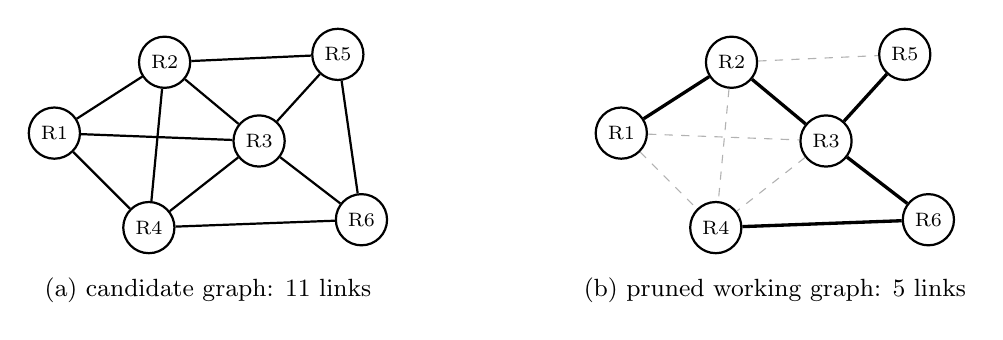
\begin{tikzpicture}[
  rover/.style={circle, draw, thick, fill=white, minimum size=6.5mm, inner sep=0pt, font=\scriptsize},
  weak/.style={gray!60, dashed},
  kept/.style={very thick},
]
\begin{scope}
\node[rover] (a) at (0,0) {R1};
\node[rover] (b) at (1.4,0.9) {R2};
\node[rover] (c) at (2.6,-0.1) {R3};
\node[rover] (d) at (1.2,-1.2) {R4};
\node[rover] (e) at (3.6,1.0) {R5};
\node[rover] (f) at (3.9,-1.1) {R6};
\foreach \u/\v in {a/b,a/c,a/d,b/c,b/d,c/d,b/e,c/e,c/f,d/f,e/f}{\draw[thick] (\u) -- (\v);}
\node[font=\small] at (1.95,-2.0) {(a) candidate graph: 11 links};
\end{scope}
\begin{scope}[xshift=7.2cm]
\node[rover] (a) at (0,0) {R1};
\node[rover] (b) at (1.4,0.9) {R2};
\node[rover] (c) at (2.6,-0.1) {R3};
\node[rover] (d) at (1.2,-1.2) {R4};
\node[rover] (e) at (3.6,1.0) {R5};
\node[rover] (f) at (3.9,-1.1) {R6};
\foreach \u/\v in {a/c,a/d,b/c,b/d,c/d,b/e}{\draw[weak] (\u) -- (\v);}
\foreach \u/\v in {a/b,b/c,c/e,c/f,d/f}{\draw[kept] (\u) -- (\v);}
\node[font=\small] at (1.95,-2.0) {(b) pruned working graph: 5 links};
\end{scope}
\end{tikzpicture}
\caption{The pruning idea: of the links in range (a), a small connected subset
is kept (b, solid) subject to link caps, a cost budget and connectivity of the
mission rovers.}
\label{fig:intro:pruning}
\end{figure}

\section{Challenges}

\begin{enumerate}[label=\arabic*.]
\item \textbf{Volatile links.} A link can get better, get worse or vanish as
rovers move, as interference changes and as distances grow. For this reason the
model also has to track how recently each link was heard.
\item \textbf{Hidden, drifting reliability.} Nobody can measure how reliable a
rover is. We can only estimate it from the tasks it was given, and which tasks
it was given depended on how much we trusted it in the first place.
\item \textbf{Scarce fog compute.} Message passing costs grow with the number
of edges, and the fog device has a small budget per cycle.
\item \textbf{Global constraints.} Whether the link caps, the processing
budget and the connectivity of the mission rovers are respected depends on the
kept graph as a whole. A rule that looks at one edge at a time has no way to
guarantee any of them.
\item \textbf{Solver reliability.} Even a correctly encoded problem does not
help if the solver gives back infeasible or weak answers, and this kind of
failure is only noticed when the answers are compared with an exact
solution.
\end{enumerate}

\section{Project Statement}

To design, implement and evaluate a pipeline for dynamic rover networks that
(i) prunes the communication graph every cycle with a constrained QUBO that
enforces degree, budget and connectivity constraints exactly; (ii) solves it
reliably and checks the solver against exact classical ground truth; (iii)
assigns tasks with a trust-aware GNN whose trust is learned online; (iv)
demonstrates the pipeline in a physics simulator and an interactive real-time
3D engine; and (v) reports honestly where the architecture pays off and where
simpler alternatives are as good or better.

\section{Objectives}

\begin{enumerate}[label=\arabic*.]
\item Formulate a constrained QUBO for dynamic graph pruning with exact,
flow-based connectivity, and verify it against an independent re-derivation
and exhaustive enumeration.
\item Explain why bit-level annealers fail on penalty-encoded QUBOs and build a
solver that reliably returns feasible, near-optimal edge sets.
\item Set up exact classical baselines so that each claim about a solver can
be checked against them.
\item Design a trust-weighted message-passing GNN with an online trust model,
cheap enough for a fog device.
\item Build a causal closed-loop simulator with a statistically sound
evaluation protocol, and a hostile automated test suite.
\item Deploy the pipeline in Gazebo with ROS~2 and in an interactive 3D
simulation engine with live tuning and side-by-side comparisons.
\end{enumerate}

\section{Scope}

The project covers the QUBO pruner, the trust-aware GNN and assignment, the
three-tier architecture, the test suite, the Gazebo and ROS~2 integration and
the 3D engine. Quantitative claims come from the statistical simulator, with
10 rovers for end-to-end experiments and 10 to 50 for scaling. Out of scope
are experiments on physical rovers (a four-rover testbed is designed but not
built), execution on quantum hardware (the QUBO matrix is exported but was not
run on a quantum processor) and channel-accurate radio modelling.

\section{Contributions}

\begin{enumerate}[label=\arabic*.]
\item A constrained QUBO for dynamic graph pruning in which connectivity is
enforced exactly by a single-commodity flow encoding (Chapter~\ref{ch:qubo}).
\item A quantitative account of the \emph{penalty barrier}: four serious
annealing samplers find the exact optimum on only 48 to 64\% of verifiable
instances, while a feasibility-projected annealer finds it on all of them
(Chapter~\ref{ch:solvers}).
\item Exact classical baselines showing that a direct mixed-integer program is
exact and about 100 times faster, which fixes the QUBO's honest role as a
hardware-target encoding (Chapter~\ref{ch:exact}).
\item A trust-aware assignment layer that beats a trust-only baseline by 8.1
points of mission success with a confidence interval excluding zero
(Chapters~\ref{ch:gnn} and~\ref{ch:results}).
\item A causal evaluation with constraint-aware baselines, a ten-level
constraint-pressure sweep, and an audit that caught a silent budget
relaxation in the project's own earlier results
(Chapters~\ref{ch:sim}--\ref{ch:results}).
\item Two deployments: a containerised Gazebo Harmonic and ROS~2 Jazzy world
(Chapter~\ref{ch:gazebo}) and an interactive 3D engine with provably
collision-free motion and a seven-draw-call renderer (Chapter~\ref{ch:engine}).
\end{enumerate}

\section{Organization of the Report}

Chapter~\ref{ch:background} surveys the background and related work, and
Chapter~\ref{ch:arch} presents the system model. Chapters~\ref{ch:qubo}
to~\ref{ch:exact} form the optimisation core: formulation, solvers and exact
baselines. Chapter~\ref{ch:gnn} covers trust-aware inference and assignment,
Chapter~\ref{ch:sim} the simulator and methodology, Chapter~\ref{ch:verify}
verification, and Chapter~\ref{ch:results} the results.
Chapters~\ref{ch:gazebo} and~\ref{ch:engine} describe the Gazebo integration
and the 3D engine, and Chapter~\ref{ch:conclusion} concludes.

\chapter{Background and Literature Survey}
\label{ch:background}

\section{Introduction}

This chapter introduces the foundations the project builds on, in three
groups: learning (graph neural networks and trust), optimisation (QUBO models,
annealing, tabu search and mixed-integer programming) and systems (the
mist--fog--cloud split, robot middleware and real-time 3D rendering). It then
surveys the closest related work and states the research gap.

\section{Graph Neural Networks}

A graph neural network learns a representation of every node by repeatedly
aggregating information from its neighbours. Kipf and Welling~\cite{kipf2017}
popularised the graph convolutional network and Hamilton
et~al.~\cite{hamilton2017} extended it to inductive settings. Most variants fit
the \emph{message-passing} template, in which node $i$ combines its own state
$h_i$ with an aggregate of its neighbours' states:
\begin{equation}
m_i=\mathop{\mathrm{AGG}}_{j\in\mathcal N(i)} h_j,\qquad h_i'=\phi(h_i,m_i),
\label{eq:bg:mp}
\end{equation}
with a permutation-invariant $\mathrm{AGG}$ and a learned update $\phi$. Two
properties matter here: inference cost is proportional to the number of edges,
so pruning saves fog compute; and weighting messages by link trust and quality
lets a node discount neighbours it cannot rely on.

\section{QUBO Models and the Penalty Method}

A quadratic unconstrained binary optimisation problem asks for
$z\in\{0,1\}^N$ minimising
\begin{equation}
H(z)=z^{\top}Qz+\mathrm{const}
\label{eq:bg:qubo}
\end{equation}
for a symmetric matrix $Q$; since $z_k^2=z_k$, the diagonal holds linear terms.
The substitution $z_k=(1+\sigma_k)/2$ with spins $\sigma_k\in\{-1,+1\}$ gives
an Ising model, so the same problem runs on classical, quantum-inspired and
quantum annealers. Glover et~al.~\cite{glover2019} and Lucas~\cite{lucas2014}
survey formulation techniques. A QUBO has no constraints, so constraints become
penalties: an equality $\sum_ka_kx_k=b$ adds $\rho(\sum_ka_kx_k-b)^2$, and an
inequality first gains a non-negative integer slack written in binary. The
weight $\rho$ must make every violation unprofitable; Chapter~\ref{ch:solvers}
shows the price of that safety.

\section{Annealing, Tabu Search and Exact Solvers}

Simulated annealing~\cite{kirkpatrick1983} proposes small changes and accepts
an uphill move of $\Delta E$ with probability $\exp(-\Delta E/\tau_{\mathrm{SA}})$
while the temperature $\tau_{\mathrm{SA}}$ is lowered; D-Wave's Ocean
software~\cite{ocean} provides the production \emph{neal} sampler. Quantum
annealing~\cite{kadowaki1998} replaces thermal fluctuations with tunnelling
driven by a transverse field, and simulated quantum annealing emulates it
classically; the OpenJij library~\cite{openjij} provides such a sampler. Tabu
search~\cite{glover1989} is a local search that forbids recent moves to escape
local minima. All four change a few bits of $z$ at a time, the property that
decides their fate in Chapter~\ref{ch:solvers}.

A mixed-integer linear program (MILP) minimises a linear objective under
linear constraints with some integer variables, and branch-and-cut solvers such
as CBC~\cite{cbc} solve it exactly with a certificate of optimality.
Connectivity of a required node set has a compact MILP form, a
\emph{single-commodity flow} in which a root sends one unit to each required
node over selected edges; network-flow theory~\cite{ahuja1993} guarantees
integral flows for integral data, so flow variables can stay continuous.

\section{Fog Computing, Trust and Task Allocation}

Bonomi et~al.~\cite{bonomi2012} describe fog computing as a tier between
devices and the cloud that places computation near the data; the deployment
here follows that split. Trust and reputation models estimate reliability from
observed behaviour; Sabater and Sierra~\cite{sabater2005} review computational
trust models and Ingole et~al.~\cite{ingole2023} survey trust in multi-robot
systems. The cheapest useful model is an exponentially weighted moving average
of outcomes. When trust is estimated without any graph, choosing the most
trusted rover is a multi-armed bandit problem~\cite{auer2002}, so a trust-only
baseline is the strongest simple competitor and is included explicitly. In the
taxonomy of Korsah et~al.~\cite{korsah2013}, our setting has single-task robots,
single-robot tasks and instantaneous assignment, recomputed every cycle.

\section{Robot Simulation and Real-Time Rendering}

ROS~2~\cite{macenski2022} is the standard robot middleware: programs are
\emph{nodes} exchanging typed messages over named \emph{topics}. Gazebo~\cite{koenig2004}
is an open-source multi-robot simulator; its current generation, Gazebo
Harmonic, describes worlds and robots in the Simulation Description Format
(SDF), and a bridge forwards its state into ROS~2. In the browser, WebGL exposes
the GPU and three.js~\cite{threejs} manages scenes on top of it. The decisive
performance quantity is the number of \emph{draw calls}, each carrying fixed
driver overhead; \emph{instanced rendering} draws many copies of a geometry in
one call, and \emph{geometry merging} combines parts that share a material.
Chapter~\ref{ch:engine} uses both to keep the whole fleet within a handful of
calls.

\section{Survey of Related Work}

Several works prune the input graph of a GNN. STEP~\cite{li2023step} learns a
self-supervised pruner for large dynamic graphs but uses graph statistics
alone, without telemetry such as trust, link quality or battery.
CGP~\cite{liu2024cgp} co-sparsifies structure, features and weights during
training, Wang et~al.~\cite{wang2022} score edges by their effect on the loss,
and Peng et~al.~\cite{peng2022} sparsify GNN weights and structure; all target
model or training efficiency on static benchmarks, and spectral
sparsification~\cite{spielman2011} preserves spectra without hard
constraints. On the allocation side, Ahanger et~al.~\cite{ahanger2023} use a
quantum-inspired optimiser for IoT task allocation across edge and fog nodes,
MAG-Q~\cite{verma2026} combines graph attention, actor--critic learning and
QUBO forwarding for task offloading in fog clusters, and Ali
et~al.~\cite{ali2023} and STMTO~\cite{guo2021} use trust for load balancing and
UAV offloading. Table~\ref{tab:bg:related} summarises them.

\begin{table}[htbp]
\centering
\caption{Qualitative comparison of related work with the present project.}
\label{tab:bg:related}
\small
\begin{tabularx}{\linewidth}{@{}l X X@{}}
\toprule
Work & Main focus & Gap relative to this project \\
\midrule
STEP~\cite{li2023step} & unsupervised pruning of large dynamic graphs & no telemetry, trust or hard constraints \\
CGP~\cite{liu2024cgp} & gradual co-sparsification in training & training-time, static benchmarks \\
Wang et~al.~\cite{wang2022} & edge scoring by effect on the loss & model-side efficiency only \\
Peng et~al.~\cite{peng2022} & weight and structural sparsification & no adaptive physical-graph pruning \\
Ahanger et~al.~\cite{ahanger2023} & quantum-inspired IoT allocation & no trust-aware GNN pruning \\
MAG-Q~\cite{verma2026} & GAT, actor--critic, QUBO forwarding & routing and placement, not pruning \\
Ali et~al.~\cite{ali2023} & trust-aware load balancing in MEC & trust is a scheduler input \\
STMTO~\cite{guo2021} & trust-aware UAV offloading & no GNN-propagated trust or sparsification \\
\midrule
This project & constrained QUBO pruning, trust GNN, solver audit, two simulators & physical testbed and quantum hardware pending \\
\bottomrule
\end{tabularx}
\end{table}

\section{Research Gap}

To our knowledge, constrained QUBO pruning combined with online trust-aware
GNN inference for rover task allocation has not been reported, and three gaps
remain open: pruning methods do not enforce hard combinatorial constraints;
trust-aware allocation methods do not propagate trust through message passing;
and QUBO applications seldom validate solver output against exact ground
truth, so solver failures can be mistaken for properties of a formulation. This
project addresses all three and adds what most proposals omit, an honest
comparison against the strongest classical alternative.

\section{System Architecture}
\label{sec:architecture}

This chapter describes how the complete system is organised: the three
physical tiers on which computation runs, the data flow within and across
those tiers, the inventory of software components, and the design rules
that shaped every implementation decision. The architecture is deliberately
asymmetric. Almost all intelligence lives on one small computer that is
physically co-located with the rover fleet, while the rovers themselves
stay minimal and the cloud is used only where its latency does not matter.

\subsection{The Three-Tier Deployment Model}
\label{sec:architecture-tiers}

We adopt the mist/fog/cloud hierarchy that is standard in edge computing
for robotics, and map our pipeline onto it as follows.

\paragraph{Mist tier: the rovers.}
Each rover carries an ESP-NOW radio and a microcontroller with limited
memory and no floating-point acceleration to speak of. The rover's
responsibilities are confined to sensing (link quality to neighbours,
battery state, odometry), executing the motion commands implied by an
assigned task, and reporting task outcomes back to the fog node. No
optimisation, no graph reasoning, and no learning happens on a rover.
This choice reflects the hardware we target: a rover that must be cheap
enough to lose in the field cannot host an annealer or a neural network.
ESP-NOW provides short-range, low-power, peer-to-peer frames without the
overhead of an association-based protocol, which suits the dense, rapidly
changing local topologies we study.

\paragraph{Fog tier: the fleet brain.}
A single Raspberry Pi class computer sits within radio range of the fleet
and runs the entire per-cycle decision loop: it assembles the candidate
graph from rover reports, formulates and solves the constrained QUBO edge
pruning problem, scores rovers with the trust-aware GNN on the pruned
graph, and performs the greedy capacity-aware task assignment. This tier
is the reason for the most consequential engineering constraint of the
project: \emph{all per-cycle numerical code is pure NumPy over tiny
matrices}. A cycle must complete in well under the control period on a
few-watt ARM processor, so there is no room for a deep learning
framework, a sparse linear algebra stack, or a commercial solver. Every
matrix in the inference path is small enough that dense NumPy with a
handful of temporaries is both the simplest and the fastest honest
option. The message-passing round of the GNN is a single adjacency
product followed by an elementwise nonlinearity, and the projected edge
annealer manipulates flat bit vectors and small dictionaries rather than
any external optimisation library.

\paragraph{Cloud tier: training, amortised solves, analytics.}
Anything whose latency does not couple into the control loop is pushed to
the cloud tier. Three workloads live there. First, offline training of the
GNN readout layer on logged outcomes; we report in Chapter 6 that this
training did not beat the fixed readout on held-out data, but the
infrastructure remains part of the architecture. Second, amortised heavy
solves: the pruning QUBO can be re-solved every $k$ cycles rather than
every cycle, and heavy verification solves (the exact MILP baseline, or
cross-checks of annealer output) are cloud jobs, not field jobs. Third,
fleet-level analytics over mission logs.

Figure~\ref{fig:tiers} summarises the deployment and the data that crosses
tier boundaries.

\begin{figure}[ht]
\centering
\resizebox{0.95\textwidth}{!}{%
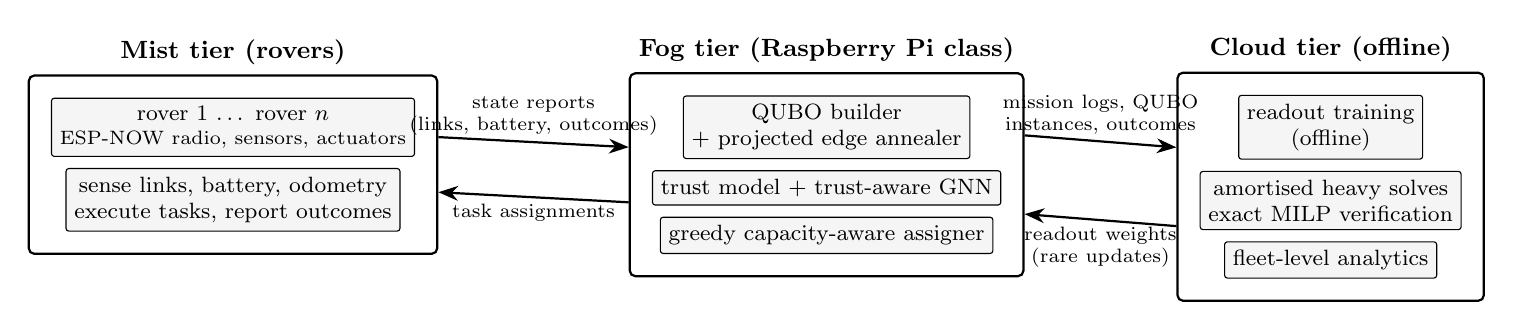
\begin{tikzpicture}[
  font=\small,
  tier/.style={draw, rounded corners=2pt, thick, inner sep=8pt},
  title/.style={font=\bfseries\small},
  comp/.style={draw, fill=black!4, rounded corners=1pt,
               inner sep=3pt, font=\footnotesize, align=center},
  flow/.style={-{Stealth[length=2.5mm]}, thick},
  lbl/.style={font=\scriptsize, align=center, inner sep=2pt},
]
% --- Mist tier box ---
\node[comp] (rovers) at (0,1.0) {rover 1 \ldots\ rover $n$\\[-1pt]
  \scriptsize ESP-NOW radio, sensors, actuators};
\node[comp, below=4pt of rovers] (mistnote) {sense links, battery, odometry\\
  execute tasks, report outcomes};
\begin{scope}[on background layer]
  \node[tier, fit=(rovers)(mistnote), label={[title]north:Mist tier (rovers)}] (mist) {};
\end{scope}

% --- Fog tier box ---
\node[comp, right=3.4cm of rovers] (qubo) {QUBO builder\\+ projected edge annealer};
\node[comp, below=4pt of qubo] (gnn) {trust model + trust-aware GNN};
\node[comp, below=4pt of gnn] (assign) {greedy capacity-aware assigner};
\begin{scope}[on background layer]
  \node[tier, fit=(qubo)(gnn)(assign),
        label={[title]north:Fog tier (Raspberry Pi class)}] (fog) {};
\end{scope}

% --- Cloud tier box ---
\node[comp, right=3.4cm of qubo] (train) {readout training\\(offline)};
\node[comp, below=4pt of train] (heavy) {amortised heavy solves\\exact MILP verification};
\node[comp, below=4pt of heavy] (analytics) {fleet-level analytics};
\begin{scope}[on background layer]
  \node[tier, fit=(train)(heavy)(analytics),
        label={[title]north:Cloud tier (offline)}] (cloud) {};
\end{scope}

% --- Flows: mist <-> fog ---
\draw[flow] ($(mist.east)+(0,0.35)$) -- node[lbl, above]{state reports\\(links, battery, outcomes)}
  ($(fog.west)+(0,0.35)$);
\draw[flow] ($(fog.west)-(0,0.35)$) -- node[lbl, below]{task assignments}
  ($(mist.east)-(0,0.35)$);

% --- Flows: fog <-> cloud ---
\draw[flow] ($(fog.east)+(0,0.5)$) -- node[lbl, above]{mission logs, QUBO\\instances, outcomes}
  ($(cloud.west)+(0,0.5)$);
\draw[flow] ($(cloud.west)-(0,0.5)$) -- node[lbl, below]{readout weights\\(rare updates)}
  ($(fog.east)-(0,0.5)$);
\end{tikzpicture}}
\caption{Three-tier deployment. The mist tier (rovers) senses and acts;
the fog tier runs the complete per-cycle decision loop on a Raspberry Pi
class computer using pure NumPy; the cloud tier performs offline training,
amortised or verification-grade solves, and fleet analytics.}
\label{fig:tiers}
\end{figure}

\subsection{Per-Cycle Data Flow}
\label{sec:architecture-flow}

One control cycle proceeds through six stages, which we describe in order,
noting what crosses a tier boundary at each step.

\paragraph{Stage 1: graph assembly (mist to fog).}
Each rover reports its current estimate of link quality to every
neighbour it can hear, its battery level, its compute availability, and
its position estimate. These reports travel over ESP-NOW to the fog node,
which merges them with its own per-node records (trust, freshness of last
contact, task criticality, processing cost) to build the full dynamic
candidate graph: every admissible rover pair is an edge, and every edge
carries a feature vector in $[0,1]^7$ covering trust, link quality,
battery, proximity, freshness, task criticality, and processing cost.

\paragraph{Stage 2: constrained QUBO pruning (fog).}
The candidate graph is denser than the GNN needs, and dense graphs dilute
the trust signal and increase inference cost. The QUBO builder encodes
edge selection as a binary quadratic program: a linear utility per edge
(the learned-weight combination of the seven features), soft penalties
for graph size and for churn against the previous cycle's decisions, and
hard constraints with dominant penalty weights that enforce per-node
degree limits, a global processing budget, and single-commodity flow
connectivity from a root to every required node. The production solver,
the projected edge annealer, moves directly in the space of feasible edge
sets: it toggles or swaps edges and repairs each candidate via an exact
slack-and-flow recomputation, so infeasible states are never committed.
The output is a pruned subgraph plus, for auditability, the raw solution
vector and a list of any violated constraints.

\paragraph{Stage 3: trust-aware scoring (fog).}
The trust model maintains an exponentially weighted moving average of
per-node reliability, with ageing so that stale evidence decays. The GNN
takes the pruned adjacency, per-node features (trust, battery, available
compute, capability), and performs one message-passing round with a
sigmoid nonlinearity, then a linear readout scores each rover against the
current task requirements. All of this is dense NumPy on matrices of
order $n \times n$ with $n$ the fleet size, comfortably inside the fog
compute budget.

\paragraph{Stage 4: assignment (fog to mist).}
A greedy capacity-aware matcher assigns tasks to the highest-scoring
rovers that still have free capacity. The assignments are radioed down to
the rovers, which execute them.

\paragraph{Stage 5: outcome sampling (mist).}
Task outcomes are realised on the rovers. In simulation, outcomes are
sampled from a hidden, spatially correlated reliability field, and the
probability of successful delivery depends causally on the pruned
topology through the paths the assignment actually uses; this design,
introduced after reviewer pressure, prevents the evaluation from being
merely correlational.

\paragraph{Stage 6: trust update (fog, then feedback).}
Reported outcomes update the trust model, closing the loop: the updated
trust values are inputs to the edge features of the next cycle. Mission
logs, QUBO instances, and outcome traces are streamed or batched to the
cloud tier for the offline workloads described above; the only
cloud-to-fog traffic in normal operation is an occasional readout-weight
update.
\subsection{Component Inventory}
\label{sec:architecture-components}

Table~\ref{tab:components} lists the components of the system by role.
Two deliberate asymmetries are worth flagging. First, two annealers exist:
a bit-level simulated annealer that manipulates raw bit strings and is
used \emph{only} as a benchmark subject, and the projected edge annealer
that is the production solver. The benchmark exists precisely because the
bit-level solver performs poorly (it cannot cross penalty barriers and
returned infeasible states on most benchmark instances), which is itself
one of our audit findings. Second, the exact MILP baseline (CBC via PuLP)
is faster and exact on our instance sizes, which we report honestly as a
negative result for QUBO on classical hardware; it serves as the ground
truth oracle for the solver audit.

\begin{table}[ht]
\centering
\caption{Component inventory. ``Tier'' indicates where the component runs
in deployment; benchmark and verification components are cloud-side or
development-side tools.}
\label{tab:components}
{\small
\begin{tabular}{@{}llll@{}}
\toprule
Component & Role & Tier & Technology \\
\midrule
QUBO builder & constrained edge-pruning encoding & fog & NumPy \\
Bit-level annealer & benchmark subject only & cloud/dev & NumPy \\
Projected edge annealer & production QUBO solver & fog & NumPy \\
Trust model & EWMA reliability with ageing & fog & NumPy \\
Trust-aware GNN & rover scoring on pruned graph & fog & NumPy \\
Greedy assigner & capacity-aware task matching & fog & NumPy \\
Exact MILP baseline & ground-truth oracle, audit & cloud & CBC via PuLP \\
Scaling runner & fleet-size experiments & cloud & NumPy \\
Hostile test suite & 491 checks, sections A to N & dev & Python stdlib \\
Causal simulation harness & end-to-end evaluation, statistics & cloud & NumPy \\
Physics integration & realistic rover dynamics & cloud & Gazebo, ROS 2, Docker \\
Fleet console & live visualisation and tuning & dev & three.js, React, Python \\
\bottomrule
\end{tabular}
}
\end{table}

The \textbf{causal simulation harness} drives the whole pipeline
end-to-end against the hidden reliability field and hosts the pruning
baselines (no pruning, threshold pruning, top-$k$ pruning, full graph)
and assignment baselines (trust-only, no-graph, random) used in the
ablation studies. It reports paired bootstrap confidence intervals and
permutation $p$-values so that every comparative claim carries an
uncertainty statement.

The \textbf{physics integration} replaces the abstract kinematics of the
simulator with Gazebo Harmonic under ROS 2 Jazzy, packaged in Docker so
that the planner node runs unmodified against simulated physics; this
validates that the fog-side loop tolerates realistic sensing noise and
actuation latency.

The \textbf{fleet console} is a browser application: a custom three.js
rendering engine (instanced meshes, a single instanced shader draw for
link arcs) with a React interface and Zustand state management, served by
a Python standard-library HTTP backend that steps live simulation
sessions and exposes in-place parameter tuning. It exists for
demonstration and for interactive exploration of solver parameters, and
its comparison menu names the baselines that beat our pipeline rather
than hiding them.

The \textbf{hostile test suite} deserves special mention as an
architectural component rather than an afterthought. Its 491 checks,
organised into sections A to N, include an independent re-derivation of
the QUBO energy that is cross-verified against the quadratic form itself,
brute-force enumeration of small instances as ground truth, exact MILP
cross-checks on larger instances, and sensitivity sweeps over annealer
hyperparameters and penalty scales.

\subsection{Design Rules}
\label{sec:architecture-rules}

Four rules, adopted early and enforced throughout, explain most of the
concrete choices above.

\paragraph{Rule 1: the fog compute budget is real.}
Every per-cycle component must run in milliseconds on a Raspberry Pi
class machine. This rules out deep learning frameworks (hence a GNN that
is one dense message-passing round in NumPy), rules out heavy sparse or
optimisation libraries in the inference path (hence a hand-rolled
projected annealer), and motivates QUBO pruning in the first place: the
pruned graph is cheaper to score, so the pruner partially pays for
itself.

\paragraph{Rule 2: no heavy dependencies anywhere.}
The numerical stack depends on NumPy alone. The exact baseline uses PuLP
with CBC, both permissively licensed and installable without system
libraries; notably, we avoid SciPy entirely. The web backend uses only
the Python standard library. The physics simulator is containerised with
Docker precisely so that its heavier ROS 2 dependency chain is isolated
from the numerical core.

\paragraph{Rule 3: every claim is paired with a test.}
The 491-check hostile suite is co-developed with the code, not appended
to it. The solver exactness rates quoted in later chapters are enforced
by floor checks in the suite, the simulation statistics are regression
checked, and new components are expected to arrive with their own hostile
tests.

\paragraph{Rule 4: negative results are kept.}
The architecture is an audit, not only a proposal, and the system is
built to surface unfavourable comparisons rather than suppress them. The
exact MILP baseline that dominates the QUBO solver on classical hardware
is a first-class component; the readout-training null result is reported
with its $p$-value; the pruner comparison in which threshold pruning wins
on raw mission success at the ten-rover scale appears in the results with
its significance test. We regard these findings as outputs of the system,
on equal footing with its successes.

\subsection{Summary}
The system places a complete decision loop on one modest fog computer by
discipline rather than by excess compute: a minimal mist tier, a
NumPy-only fog tier running pruning, scoring, and assignment, and a
cloud tier reserved for training, verification-grade solves, and
analytics. The
surrounding tooling, from the MILP oracle to the hostile suite to the
fleet console, exists to make the central claims falsifiable and the
negative results impossible to misplace.

\chapter{Constrained QUBO Formulation}
\label{ch:qubo}

\section{Overview}

The pruning stage chooses, in every cycle, which edges of $G_t$ to keep. The
choice is combinatorial: it must maximise the usefulness of the kept edges
while respecting per-rover degree caps, a global cost budget and the
connectivity of a set of required rovers. This chapter writes that problem as
a single QUBO, explains every term, proves the two properties that make the
encoding correct, works through a five-rover example by hand and reports how
the implementation was verified.

\section{Decision Variables and Notation}

Let $H\subseteq E_t$ be the \emph{hard-critical} edges, which are always kept
(for example a relay rover's only link), and $O=E_t\setminus H$ the optional
edges. Let $R$ be the required rovers with root $r\in R$ and $m=|R|-1$, let
$D_i$ be the degree cap of rover $i$, and let $K$ be the global budget in
integer cost units. Writing $\deg_H(i)$ for the number of hard edges at $i$
and $c_H$ for their total cost, the remaining degree capacity of rover $i$ is
$D_i-\deg_H(i)$ and the remaining budget is $K-c_H$.
Table~\ref{tab:qubo:vars} lists the four families of binary variables.

\begin{table}[htbp]
\centering
\caption{Variable families of the QUBO. Every integer is binary-encoded.}
\label{tab:qubo:vars}
\small
\begin{tabularx}{\linewidth}{@{}l X l@{}}
\toprule
Variable & Meaning & Number of bits \\
\midrule
$x_e,\ e\in O$ & keep (1) or prune (0) optional edge $e$ & $|O|$ \\
$s_i,\ i\in V$ & degree slack, $0\le s_i\le D_i-\deg_H(i)$ & $\sum_i\lceil\log_2(D_i-\deg_H(i)+1)\rceil$ \\
$s_C$ & budget slack, $0\le s_C\le K-c_H$ & $\lceil\log_2(K-c_H+1)\rceil$ \\
$f_{uv},f_{vu},q_e,\ e\in E_t$ & two directed flows and a capacity slack per edge, each in $[0,m]$ & $3|E_t|\lceil\log_2(m+1)\rceil$ \\
\bottomrule
\end{tabularx}
\end{table}

For notational convenience $x_e:=1$ for $e\in H$. The vector $z$ stacks all
bits, and $N$ denotes its length.

\section{The Energy Function}

The complete energy is
\begin{align}
H(z) ={}& \sum_{e\in O}(-U_e+\lambda)\,x_e
 + \eta\sum_{e\in O}\bigl(x_e-x_e^{t-1}\bigr)^2 \notag\\
&+ \rho_d\sum_{i\in V}\Bigl(\sum_{e\in\delta_O(i)}x_e+s_i-\bigl(D_i-\deg_H(i)\bigr)\Bigr)^2 \notag\\
&+ \rho_C\Bigl(\sum_{e\in O}c_ex_e+s_C-(K-c_H)\Bigr)^2 \notag\\
&+ \rho_F\sum_{v\in V}\bigl(\mathrm{in}_v-\mathrm{out}_v-b_v\bigr)^2 \notag\\
&+ \rho_{FC}\sum_{e=(u,v)\in E_t}\bigl(f_{uv}+f_{vu}+q_e-m\,x_e\bigr)^2,
\label{eq:qubo:energy}
\end{align}
where $\delta_O(i)$ is the set of optional edges at rover $i$; the total flows
entering and leaving rover $v$ are $\mathrm{in}_v$ and $\mathrm{out}_v$; and
the supplies are $b_r=-m$, $b_v=1$ for $v\in R\setminus\{r\}$ and
$b_v=0$ otherwise. Each squared bracket is a polynomial of degree two in the
bits, so the whole expression expands into the form $z^{\top}Qz+\mathrm{const}$.
Table~\ref{tab:qubo:consts} collects the constants.

\begin{table}[htbp]
\centering
\caption{Constants of the QUBO used throughout the report.}
\label{tab:qubo:consts}
\small
\begin{tabularx}{\linewidth}{@{}l X r@{}}
\toprule
Constant & Role & Value \\
\midrule
$\lambda$ & sparsity penalty per kept edge & 0.08 \\
$\eta$ & stability penalty per changed decision & 0.15 \\
$\rho_d,\ \rho_C$ & degree and budget penalty weights & 100 \\
$\rho_F,\ \rho_{FC}$ & flow conservation and flow capacity weights & 500 \\
cost scale & quantisation of $\bar c_e$ into budget units & 10 \\
utility weights & trust, link, battery, proximity, freshness, task & 0.25, 0.25, 0.10, 0.10, 0.15, 0.15 \\
\bottomrule
\end{tabularx}
\end{table}

\section{The Soft Terms}

The coefficient $-U_e+\lambda$ rewards an edge for its utility and charges a
constant $\lambda$ for keeping it, so edges with $U_e<\lambda$ are never worth
keeping alone and the constant pressure drives solutions towards sparse
graphs. The stability term charges $\eta$ for every decision that changes
relative to the previous cycle; since $x_e^2=x_e$ it is linear,
$\eta\bigl(x_e(1-2x_e^{t-1})+x_e^{t-1}\bigr)$, and it stops the kept topology
from flapping between nearly equal alternatives, which would confuse both the
GNN and the trust model.

\section{Encoding Inequalities with Slack}

Degree caps and the budget are inequalities. The standard device turns
$\sum_k a_kx_k\le B$ into the equality $\sum_k a_kx_k+s=B$ with an integer
slack $0\le s\le B$, writes $s=\sum_j 2^js_j$ in bits, and penalises the
squared residual. Expanding a single squared constraint
$(a^{\top}y-B)^2$ over a bit vector $y$ and using $y_k^2=y_k$ gives
\begin{equation}
(a^{\top}y-B)^2=\sum_k\bigl(a_k^2-2Ba_k\bigr)y_k+2\sum_{k<l}a_ka_ly_ky_l+B^2,
\label{eq:qubo:expand}
\end{equation}
so a constraint contributes $a_k^2-2Ba_k$ to the diagonal entry of each of its
bits, $a_ka_l$ to each symmetric off-diagonal pair, and $B^2$ to the
constant.

\begin{example}[One degree constraint]
Take a rover with cap $D_i=2$, no hard edges and three optional edges
$x_1,x_2,x_3$. The slack $s_i\in\{0,1,2,3\}$ needs two bits, $s_i=s_0+2s_1$,
so the coefficient vector over $(x_1,x_2,x_3,s_0,s_1)$ is $a=(1,1,1,1,2)$ and
$B=2$. Equation~\eqref{eq:qubo:expand} yields the entries of
Table~\ref{tab:qubo:degree}, all multiplied by $\rho_d$.
\end{example}

\begin{table}[htbp]
\centering
\caption{Coefficients generated by one degree constraint with $D_i=2$
(before multiplication by $\rho_d$).}
\label{tab:qubo:degree}
\small
\begin{tabular}{@{}l r l@{}}
\toprule
Bit & Linear term $a_k^2-2Ba_k$ & Pairwise term $2a_ka_l$ \\
\midrule
$x_1,x_2,x_3$ & $-3$ each & 2 with each other and with $s_0$; 4 with $s_1$ \\
$s_0$ & $-3$ & 2 with each $x$; 4 with $s_1$ \\
$s_1$ & $-4$ & 4 with each $x$ and with $s_0$ \\
constant & $B^2=4$ & \\
\bottomrule
\end{tabular}
\end{table}

Three checks confirm the intended behaviour. Keeping two edges with both
slack bits zero gives $(2-2)^2=0$. Keeping one edge with $s_0=1$ also gives
$0$. Keeping all three edges gives at least $(3-2)^2=1$ for every slack
setting, because slack cannot be negative; the violation therefore costs at
least $\rho_d=100$, while the third edge can gain at most about $1.2$.

\section{The Budget Constraint}

The budget term has the same structure, with the integer costs $c_e$ as
coefficients and $K-c_H$ as right-hand side, and its slack needs only
$\lceil\log_2(K-c_H+1)\rceil$ bits. A budget below the cost of every connected
subgraph is \emph{infeasible} together with connectivity, and no penalty
weighting can change that; Section~\ref{sec:sol:ladder} shows how the
production solver detects and records this case, and
Section~\ref{sec:res:audit} shows that the project's own earlier experiments
fell into exactly this trap.

\section{Exact Connectivity by Single-Commodity Flow}

The two flow terms enforce connectivity of the required set inside the
optimisation itself, rather than through a check applied afterwards.

\begin{proposition}[Flow encodes connectivity]
Let $x$ be a selection of edges. There exist integer flows and slacks that
make both flow terms of Eq.~\eqref{eq:qubo:energy} zero if and only if every
required rover is connected to the root $r$ in the subgraph of selected
edges.
\end{proposition}

\begin{proof}
($\Leftarrow$) If every required rover is connected to $r$, choose a spanning
tree of the root's component and route one unit from $r$ to each required
rover along its unique tree path. Every arc then carries at most $m$ units,
conservation holds at every node with the given supplies, and each selected
edge satisfies $f_{uv}+f_{vu}\le m$, so a slack $q_e\in[0,m]$ closes the
capacity equality. Unselected edges carry no flow and take $q_e=0$.
($\Rightarrow$) If both terms are zero, conservation says that $m$ units leave
$r$ and one unit is absorbed at each other required rover, while capacity
forces $f_{uv}=f_{vu}=0$ on every unselected edge. Decomposing the flow into
paths, each required rover receives its unit along a path of selected edges
from $r$, so it is connected to $r$.
\end{proof}



\section{Why the Penalties Dominate}

\begin{proposition}[No violation is profitable]
With $\rho_d=\rho_C=100$, $\rho_F=\rho_{FC}=500$ and soft coefficients of
magnitude at most about $1.2$ per edge, every exact minimiser of
Eq.~\eqref{eq:qubo:energy} satisfies all constraints whenever a feasible
selection exists.
\end{proposition}

\begin{proof}[Argument]
A violated degree or budget constraint contributes at least $\rho=100$,
because its residual is a non-zero integer and enters squared, while each unit
of violation unlocks at most one edge worth less than $1+\lambda+\eta<1.25$.
Flow violations are penalised quadratically against an at most linear gain.
\end{proof}

The argument is confirmed exhaustively in Section~\ref{sec:qubo:verify}.
It also explains the difficulty of Chapter~\ref{ch:solvers}: the same walls
that make violations unprofitable make them unreachable for a sampler that
must climb over them.

\section{A Worked Example on Five Rovers}
\label{sec:qubo:worked}

The whole formulation is visible on an instance small enough to solve by
hand. There are five rovers: the root $0$ and rovers $1$ to $4$. Seven links
are in range. The link $0$--$1$ is hard-critical, being rover~1's only
tether. Rovers $\{0,2,3,4\}$ are required, so rover~1 is a relay that may be
cut off. The degree caps are $(3,2,3,2,2)$ for rovers $0$ to $4$ and the
budget is $K=12$ units. Table~\ref{tab:qubo:worked} gives the utility, the
integer cost and the previous decision of every link.

\begin{table}[htbp]
\centering
\caption{The five-rover worked example: utility $U_e$ from
Eq.~\eqref{eq:arch:utility}, integer cost $c_e$ and previous-cycle decision
$x_e^{t-1}$.}
\label{tab:qubo:worked}
\small
\begin{tabular}{@{}l r r r@{}}
\toprule
Link & $U_e$ & $c_e$ & $x_e^{t-1}$ \\
\midrule
$0$--$1$ (hard) & 0.810 & 2 & 1 \\
$0$--$2$ & 0.900 & 1 & 1 \\
$0$--$3$ & 0.405 & 8 & 0 \\
$1$--$2$ & 0.705 & 3 & 1 \\
$2$--$3$ & 0.750 & 4 & 1 \\
$2$--$4$ & 0.790 & 2 & 0 \\
$3$--$4$ & 0.555 & 6 & 1 \\
\bottomrule
\end{tabular}
\end{table}

\subsubsection{Size} There are six optional edges. With $m=3$ every flow
integer needs two bits, so the flow family has $3\times7\times2=42$ bits; the
degree slacks need $2+1+2+2+2=9$ bits and the budget slack, with $K-c_H=10$,
needs 4. The QUBO therefore has $6+42+9+4=61$ binary variables, even though
the decision itself has only $2^6=64$ possibilities.

\subsubsection{Enumeration} All 64 optional-edge subsets were enumerated.
Only \textbf{3} are feasible. The optimum keeps $\{0\text{--}1,0\text{--}2,
2\text{--}3,2\text{--}4\}$ at a cost of 9 units, with energy
\[
\underbrace{(-0.82)+(-0.67)+(-0.71)}_{\text{utility and sparsity}}
+\underbrace{0.15\times3}_{\text{stability}}=-1.750,
\]
where the three stability charges come from dropping $1$--$2$ and $3$--$4$
and adding $2$--$4$. The other two feasible subsets both score $-1.555$.

\subsubsection{The trap} Thirty of the 61 infeasible subsets violate only
connectivity. The best of them, $\{0\text{--}1,0\text{--}2,1\text{--}2,
2\text{--}3\}$, has a \emph{lower} soft energy of $-1.965$ because it keeps
the attractive link $1$--$2$ and pays only one stability charge, but it cuts
rover~4 off from the root. A pruner that judged edges by soft score alone, or
checked connectivity only afterwards, would prefer it by $0.215$. In the QUBO
the flow terms add at least 500, so its true energy is above $+498$. The
cheapest degree or budget violator sits at $+97.475$: the barrier between it
and the optimum is $99.2$, almost a hundred times the width of the whole
feasible band ($[-1.750,-1.555]$). Fig.~\ref{fig:qubo:ladder} draws this
energy ladder.

\begin{figure}[htbp]
\centering
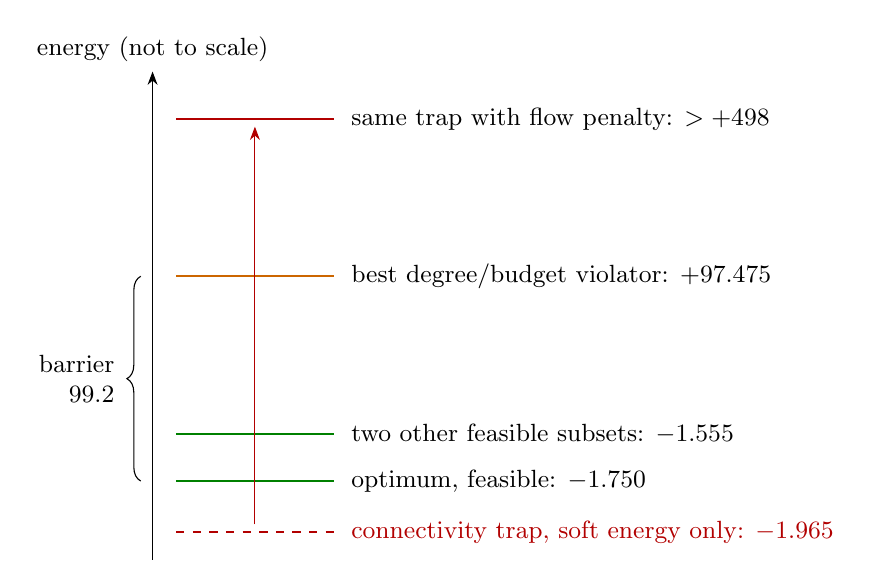
\begin{tikzpicture}[
  lvl/.style={thick},
  lab/.style={font=\small, anchor=west},
]
\draw[-{Stealth}] (0,0) -- (0,6.2) node[above, font=\small] {energy (not to scale)};
\draw[lvl, green!50!black] (0.3,1.0) -- (2.3,1.0); \node[lab] at (2.4,1.0) {optimum, feasible: $-1.750$};
\draw[lvl, green!50!black] (0.3,1.6) -- (2.3,1.6); \node[lab] at (2.4,1.6) {two other feasible subsets: $-1.555$};
\draw[lvl, red!70!black, dashed] (0.3,0.35) -- (2.3,0.35); \node[lab, red!70!black] at (2.4,0.35) {connectivity trap, soft energy only: $-1.965$};
\draw[lvl, orange!80!black] (0.3,3.6) -- (2.3,3.6); \node[lab] at (2.4,3.6) {best degree/budget violator: $+97.475$};
\draw[lvl, red!70!black] (0.3,5.6) -- (2.3,5.6); \node[lab] at (2.4,5.6) {same trap with flow penalty: $>+498$};
\draw[-{Stealth}, red!70!black] (1.3,0.45) -- (1.3,5.5);
\draw[decorate, decoration={brace, amplitude=5pt, mirror}] (-0.15,3.6) -- (-0.15,1.0) node[midway, left=6pt, font=\small, align=right] {barrier\\$99.2$};
\end{tikzpicture}
\caption[Energy ladder of the worked example.]{Energy ladder of the worked example. The connectivity trap looks
better than the optimum to a pruner that ignores connectivity; the flow
penalty lifts it far above every feasible subset.}
\label{fig:qubo:ladder}
\end{figure}

\subsubsection{Cross-checks} The Q-matrix energy of the optimum, computed as
$z^{\top}Qz+\mathrm{const}$ on the feasible bit vector, equals $-1.750$ and
matches enumeration. The production annealer of Chapter~\ref{ch:solvers}
returns the same four edges with no violations, and the exact MILP of
Chapter~\ref{ch:exact} reaches the same soft energy. Three independent
routes agree on one answer.

\section{Verification of the Encoding}
\label{sec:qubo:verify}

Two further checks were run on random instances.

\begin{enumerate}[label=\arabic*.]
\item \textbf{Exhaustive optimum check.} Over 38 randomly generated
instances, the exact bit-level optimum of Eq.~\eqref{eq:qubo:energy} never
contains a violated constraint, as the dominance argument predicts.
\item \textbf{Independent re-derivation.} The energy was re-derived from the
specification by separate code that evaluates every term directly, without
building $Q$. On 40 instances with 8 random states each, the matrix energy
agrees with the independent evaluation to within $2.3\times10^{-10}$.
\end{enumerate}

This is strong empirical validation of the implementation, not a formal
proof, and it is reported as such. It does, however, settle the attribution
question that dominates the next chapter: when a solver later returns a poor
answer, the fault lies with the solver and not with the encoding.

\section{Problem Size}

The flow family dominates the variable count, and the matrix is stored
densely, so memory grows with the square of the number of bits. On
range-limited random fleets with connectivity enforced, ten rovers give 427
binary variables (a 1.5~MB matrix) and twenty rovers 1076 variables (9.3~MB);
without connectivity, fifty rovers need only 328. The dense formulation
therefore targets tens of rovers rather than hundreds, a limit revisited in
Chapter~\ref{ch:conclusion}.

\section{Solvers: from Bit Flips to Feasibility Projection}
\label{ch:solvers}

The QUBO formulation of the previous chapter defines a discrete energy
landscape over binary vectors, one bit per optional edge plus auxiliary
slack and flow variables. This chapter asks how that landscape can be
searched, and why the answer is less obvious than the phrase ``run an
annealer'' suggests. We proceed in three steps. First we describe a
conventional bit-level simulated annealer and the samplers against which
it is benchmarked. Second, we show that this entire family of methods
performs poorly on penalty-encoded constrained instances, and we trace
the failure to a structural property of the landscape rather than to
parameter tuning. Third, we describe the production solver, a projected
annealer whose moves live inside the feasible set, and we report its
measured accuracy against exact ground truth.

\subsection{A bit-level simulated annealer}
\label{sec:bit-sa}

Our reference annealer operates directly on the raw bit string. Each
variable of the QUBO, including edge bits, integer slack bits, and
directed flow bits, is a binary decision, and a move flips one of them.
A flip changes the energy by an amount computed incrementally from the
$Q$ matrix, so a single move costs $O(n)$ in the number of variables
rather than a full quadratic energy re-evaluation. The acceptance rule
is the standard Metropolis criterion: downhill moves are taken
unconditionally, and uphill moves of magnitude $\Delta E$ are accepted
with probability $\exp(-\Delta E / T)$.

The schedule is geometric cooling. Starting from an initial temperature
$T_0 = 10$, the temperature is multiplied by a cooling rate of $0.98$
after every two sweeps, where one sweep attempts one move per variable
on average, until a final temperature of $10^{-3}$ is reached. Two
extensions round out the design. First, with a configurable pair
probability, a move flips two bits simultaneously instead of one; this
helps the sampler traverse configurations in which two compensating
changes are neutral jointly but costly individually. Second, the
annealer accepts warm initial states, so a previously discovered
configuration can seed a new run rather than starting from a random
string.

Because the word ``effort'' is otherwise easy to game, the annealer
maintains an explicit counter of energy evaluations. Every comparison in
this chapter reports that counter, so that a solver which wins by doing
more work is visibly doing more work. This habit of honest accounting
matters here, because the production solver of
Section~\ref{sec:projected} does more work per move and we want that
visible rather than hidden.

\subsection{Why bit-level annealing fails on constrained QUBOs}
\label{sec:why-fails}

The failure mode is easy to state and hard to fix within the bit-flip
paradigm. In our encoding, hard constraints are enforced by penalty
terms whose weights, between $100$ and $500$, are chosen to dominate the
soft objective: the utility of a single edge is at most about $1$, so
breaking one constraint costs at least one hundred times more than any
single edge can ever be worth. The intended consequence is that any
optimizer which minimizes total energy will respect the constraints. The
unintended consequence is that the energy landscape becomes a set of
deep, narrow valleys separated by enormous barriers.

Consider a Metropolis sampler sitting in a feasible configuration and
contemplating a single bit flip. Almost every flip that touches a
constraint variable produces a state that violates a constraint, with an
energy increase of at least $100$. At temperature $T = 1$, such a move
is accepted with probability below $e^{-100}$, which is zero for all
practical purposes. The sampler is therefore confined to the feasible
region it started in, able to leave it only at the high temperatures of
the early schedule, when acceptance is indiscriminate and no useful
signal is retained. Cooling then strands it in whichever valley it
happened to occupy. Random restarts do not rescue the method: starting
from uniformly random bit strings, the bit-level annealer returned an
infeasible final state in 19 of 25 test instances. The sampler could not
even find its way back into the feasible region, let alone optimize
within it.

We emphasize that this is not a complaint about a particular
implementation. Penalty-encoded constraints create, by construction,
barriers that single-bit moves cannot cross at useful temperatures.
Stronger cooling schedules, more sweeps, or pair moves shift the numbers
by a few percentage points but do not address the geometry.

\subsection{Sampler benchmark on the real Q matrices}
\label{sec:sampler-bench}

To quantify the claim, we benchmarked four samplers on the actual $Q$
matrices produced by our encoding for 25 representative instances, with
ground truth defined two ways. For each instance, the exact optimum of
the constrained problem was obtained by complete enumeration of the
optional-edge subsets, and the exact minimum of the encoded QUBO was
obtained by a linearized exact solve with CBC, which converts each
quadratic term into an auxiliary variable and proves optimality with a
branch-and-bound search. The two agree wherever both are computable;
the CBC solve is the ground truth for what a sampler \emph{should}
return.

Table~\ref{tab:sampler-results} summarizes the outcome. The local
bit-level annealer reaches the exact optimum in 56\% of instances.
D-Wave's \code{neal} sampler, a mature open-source simulated annealing
implementation, reaches 60\%. Tabu search reaches 64\%, the best of the
four, and simulated quantum annealing through OpenJij reaches 48\%, the
worst. No sampler clears two thirds. Figure~\ref{fig:sampler-rates}
shows the same numbers against the exact reference at 100\%.

\begin{table}[t]
  \centering
  \caption{Schedules and defaults of the solvers compared in this
  chapter. The bit-level annealer, \code{neal}, tabu, and simulated
  quantum annealing (SQA) all operate on the raw bit string of the
  encoded QUBO. The projected annealer operates on feasible edge sets;
  its temperature range is lower because its moves change the soft
  objective only.}
  \label{tab:solver-schedules}
  \small
  \begin{tabular}{lccccc}
    \toprule
    Solver & $T_{\mathrm{init}}$ & $T_{\mathrm{final}}$ &
    Cooling & Steps per $T$ & Restarts \\
    \midrule
    Bit-level SA & 10 & $10^{-3}$ & 0.98 & 2 sweeps & 1 (warm optional) \\
    \code{neal} & \multicolumn{3}{c}{default \code{beta\_range}} &
    default sweeps & 1 \\
    Tabu search & \multicolumn{3}{c}{n/a (tenure-based)} &
    default iterations & 1 \\
    SQA (OpenJij) & \multicolumn{3}{c}{default transverse-field schedule}
    & default sweeps & 1 \\
    Projected annealer & 1.0 & $10^{-2}$ & 0.998 & 4 & 5 \\
    \bottomrule
  \end{tabular}
\end{table}

\begin{table}[t]
  \centering
  \caption{Exact-solution rates on 25 instances with enumerated ground
  truth. ``Infeasible'' counts runs whose returned bit string violates
  at least one constraint. The projected annealer is excluded from this
  comparison by design; see Section~\ref{sec:projected-honesty}.}
  \label{tab:sampler-results}
  \small
  \begin{tabular}{lcc}
    \toprule
    Sampler & Exact rate & Returned infeasible \\
    \midrule
    Bit-level SA (ours) & 56\% & 19 of 25 (random restarts) \\
    \code{neal} & 60\% & n/a \\
    Tabu search & 64\% & n/a \\
    SQA (OpenJij) & 48\% & n/a \\
    \midrule
    Exact linearized solve (CBC) & 100\% (reference) & 0 \\
    \bottomrule
  \end{tabular}
\end{table}

\begin{figure}[t]
  \centering
  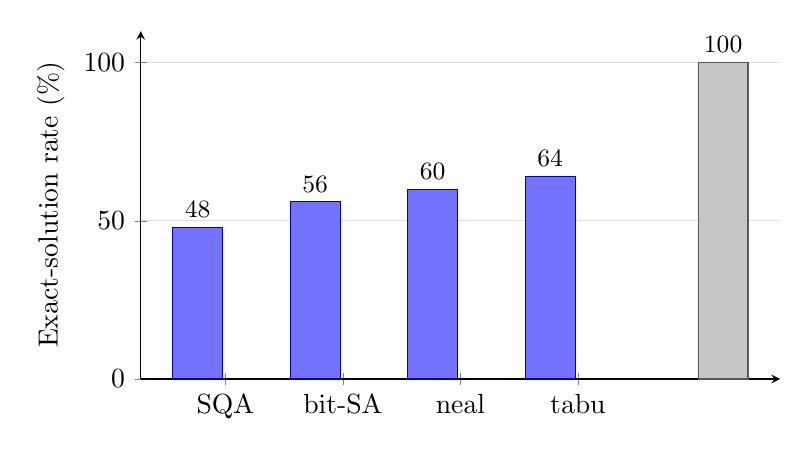
\begin{tikzpicture}
    \begin{axis}[
      ybar,
      width=0.8\textwidth,
      height=6cm,
      bar width=18pt,
      ymin=0, ymax=110,
      ylabel={Exact-solution rate (\%)},
      symbolic x coords={SQA, bit-SA, neal, tabu, exact (CBC)},
      xtick=data,
      nodes near coords,
      nodes near coords align={vertical},
      every node near coord/.append style={font=\small},
      ymajorgrids=true,
      grid style={gray!25},
      axis lines=left,
      enlarge x limits=0.18,
    ]
      \addplot[fill=blue!55, draw=blue!70!black] coordinates
        {(SQA,48) (bit-SA,56) (neal,60) (tabu,64)};
      \addplot[fill=gray!45, draw=gray!70!black] coordinates
        {(exact (CBC),100)};
    \end{axis}
  \end{tikzpicture}
  \caption{Exact-solution rates of four samplers on 25 QUBO instances
  derived from our encoding. The gray bar is the exact linearized CBC
  solve at 100\%, which defines the ground truth against which all
  sampler rates are measured; it is a reference, not a competitor.}
  \label{fig:sampler-rates}
\end{figure}

Two conclusions follow. First, the weakness is shared across
implementations and paradigms: classical annealing, tabu search, and
simulated quantum annealing all struggle, which supports the geometric
explanation of Section~\ref{sec:why-fails} over any
implementation-specific one. Second, the Q matrix itself is not at
fault, because the exact linearized solve of that same matrix recovers
the true optimum every time. The encoding is a faithful specification;
generic samplers are simply poor at searching it.

\subsection{The production solver: feasibility-projected edge annealing}
\label{sec:projected}

The production solver changes the search space rather than the search
algorithm. Instead of annealing over raw bit strings and hoping to land
inside the feasible region, it anneals directly over the set of feasible
edge subsets. A state is a set of kept edges together with the slack and
flow assignments that certify its feasibility; the energy of a state is
exactly the QUBO energy evaluated at that certificate. On the feasible
manifold the penalty terms vanish identically, so the energy reduces to
the soft objective, and the sampler never wastes a single evaluation on
a constraint violation.

Two move types generate candidates, as illustrated in
Figure~\ref{fig:moves}. A \emph{toggle} adds or removes one optional
edge. A \emph{swap} exchanges two edges, one in and one out, which
allows the solver to reallocate budget or degree capacity between parts
of the graph in a single step. Not every candidate is feasible: adding
an edge can exceed a degree cap or the global budget, and removing one
can disconnect a required node from the root. Each candidate is
therefore passed through a projection step, an exact repair procedure
that recomputes the integer slack variables and rebuilds a spanning-tree
flow certifying connectivity. If the repair succeeds, the repaired state
is the candidate actually scored; if no feasible repair exists, the move
is rejected outright. Projection is deterministic and exact, so the
solver's trajectory never leaves the feasible set.

\begin{figure}[t]
  \centering
  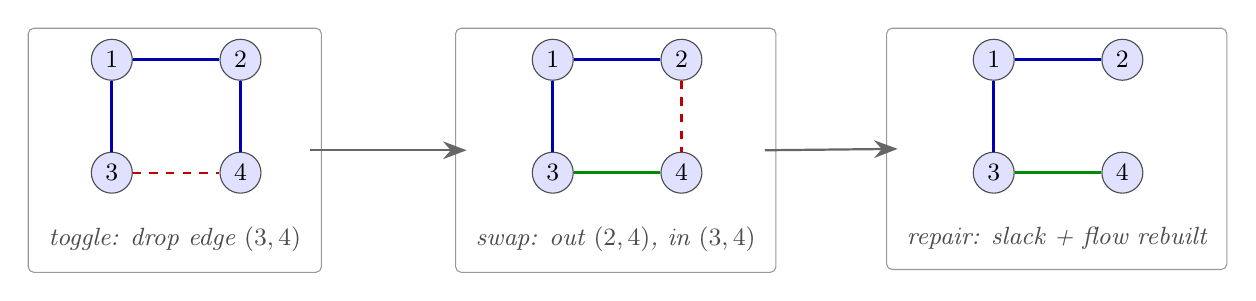
\begin{tikzpicture}[
    node distance=9mm and 11mm,
    vertex/.style={circle, draw=black!70, fill=blue!12, inner sep=1.6pt,
      minimum size=5.2mm, font=\small},
    kept/.style={draw=blue!70!black, very thick},
    gone/.style={draw=red!75!black, thick, dashed},
    added/.style={draw=green!55!black, very thick},
    panel/.style={draw=black!40, rounded corners=2pt, inner sep=4pt},
    lbl/.style={font=\small\itshape, text=black!70},
  ]
    % toggle panel
    \begin{scope}[local bounding box=toggle]
      \node[vertex] (t1) {1};
      \node[vertex, right=of t1] (t2) {2};
      \node[vertex, below=of t1] (t3) {3};
      \node[vertex, right=of t3] (t4) {4};
      \draw[kept] (t1) -- (t2);
      \draw[kept] (t1) -- (t3);
      \draw[kept] (t2) -- (t4);
      \draw[gone] (t3) -- (t4);
      \node[lbl, below=3mm of t3, xshift=8mm] {toggle: drop edge $(3,4)$};
    \end{scope}
    % swap panel
    \begin{scope}[local bounding box=swap, xshift=5.6cm]
      \node[vertex] (s1) {1};
      \node[vertex, right=of s1] (s2) {2};
      \node[vertex, below=of s1] (s3) {3};
      \node[vertex, right=of s3] (s4) {4};
      \draw[kept] (s1) -- (s2);
      \draw[kept] (s1) -- (s3);
      \draw[gone] (s2) -- (s4);
      \draw[added] (s3) -- (s4);
      \node[lbl, below=3mm of s3, xshift=8mm]
        {swap: out $(2,4)$, in $(3,4)$};
    \end{scope}
    % projection panel
    \begin{scope}[local bounding box=proj, xshift=11.2cm]
      \node[vertex] (p1) {1};
      \node[vertex, right=of p1] (p2) {2};
      \node[vertex, below=of p1] (p3) {3};
      \node[vertex, right=of p3] (p4) {4};
      \draw[kept] (p1) -- (p2);
      \draw[kept] (p1) -- (p3);
      \draw[added] (p3) -- (p4);
      \node[lbl, below=3mm of p3, xshift=8mm]
        {repair: slack + flow rebuilt};
    \end{scope}
    % arrows between panels
    \draw[-{Stealth[length=3mm]}, thick, black!60]
      (toggle.east) -- (swap.west);
    \draw[-{Stealth[length=3mm]}, thick, black!60]
      (swap.east) -- (proj.west);
    \begin{scope}[on background layer]
      \node[panel, fit=(toggle)] {};
      \node[panel, fit=(swap)] {};
      \node[panel, fit=(proj)] {};
    \end{scope}
  \end{tikzpicture}
  \caption{The move set of the projected annealer. Solid blue edges are
  kept, the dashed red edge is removed, and the green edge is added. A
  toggle changes one optional edge; a swap exchanges two. The right
  panel shows the projection step: after the move, integer slack
  variables and a spanning-tree flow from the root are recomputed
  exactly, and the candidate is accepted only if the repair succeeds.}
  \label{fig:moves}
\end{figure}

Restarts require care, for the same geometric reason that defeats
bit-level annealing. Greedy edge-by-edge growth, adding the
highest-utility edge that keeps the partial solution feasible, cannot
cross the infeasible prefix states that the connectivity constraint
creates: a cheap subtree can be constructed that is locally feasible yet
admits no feasible completion within budget. Restart states are
therefore generated as degree-cap-aware random spanning trees, sampled
so that every partial state is a tree that already respects the degree
limits, and then completed with any budget-feasible extra edges. This
guarantees that every restart begins inside the feasible manifold with a
diverse geometry.

After cooling, a deterministic polish drives the incumbent to a local
fixpoint. The polish alternates a pass of all single toggles with a pass
of all pairwise swaps, accepting every strict improvement, until neither
pass finds one. The polish is cheap relative to the anneal and removes
the residual noise that a finite temperature schedule leaves behind.

It is worth being precise about what the QUBO has become in this design.
The QUBO remains the specification of the problem: the energy function,
the constraint weights, and the feasibility test are all defined by it,
and the $Q$ matrix is still exported for hardware backends, so a quantum
or dedicated annealing device can be substituted for the classical
sampler without touching the formulation. The projected annealer is best
understood as a classical sampler that exploits the known structure of
the penalty terms to restrict itself to the subspace where those terms
are zero.

\subsection{Defaults, measured cost, and accuracy}
\label{sec:projected-results}

The production defaults are deliberately mild, because the feasible
manifold is a friendlier landscape than the raw bit space. The initial
temperature is $1.0$, the final temperature is $10^{-2}$, the cooling
rate is $0.998$, and each temperature holds for four steps. Toggles and
swaps are proposed with equal probability $0.5$. Five restarts are
drawn from the random spanning-tree generator, and in the live system
the previous cycle's kept edges are supplied as a warm start, so that
successive cycles refine an incumbent rather than restarting from
scratch.

Measured on the benchmark instances, a solve performs about $2.4 \times
10^{4}$ energy evaluations and takes about $2.1$ seconds of wall time on
commodity hardware. The accuracy numbers are the following.

\begin{itemize}
  \item \textbf{Small instances.} On the 25 instances with enumerated
  ground truth, the projected annealer returns the exact optimum in
  100\% of cases, against 56\% to 64\% for the raw-space samplers of
  Table~\ref{tab:sampler-results}.
  \item \textbf{Larger instances.} On 20 larger instances where
  enumeration is infeasible and ground truth comes from the exact MILP
  solve of the original constrained problem, the projected annealer is
  exact in 95\% of cases, with a mean true optimality gap of $7 \times
  10^{-5}$ and a worst-case gap of $1.4 \times 10^{-3}$.
  \item \textbf{Robustness.} Across a sensitivity sweep that perturbs
  the initial and final temperatures, the cooling rate, the restart
  count, the penalty scales, and the pair probability, the solver
  remains exact in 87\% of configurations. Accuracy degrades gracefully
  rather than catastrophically when the schedule is mistuned.
\end{itemize}

\subsection{An honest framing}
\label{sec:projected-honesty}

The projected annealer is not entered into the sampler comparison of
Section~\ref{sec:sampler-bench}, and we want the reason on record. Its
move set is richer than what a generic sampler is permitted: it exploits
domain knowledge, namely the structure of the constraint set, the
meaning of the slack variables, and the availability of an exact repair
procedure, that a hardware annealer or a black-box sampler acting on a
raw $Q$ matrix does not have. Comparing it against \code{neal}, tabu, or
OpenJij on equal footing would conflate two different questions: how
well generic samplers search penalty-encoded QUBOs, and how well a
structure-aware classical algorithm solves the underlying constrained
problem. The first question is the scientifically interesting one for
assessing quantum and quantum-inspired hardware, and it is answered by
Table~\ref{tab:sampler-results}. The projected annealer is therefore
reported as an engineering note: it is the solver the deployed system
actually uses, and its near-exact results establish that the QUBO
formulation itself, not any solver, is the binding constraint on
end-to-end performance. Where a classical exact optimum is affordable,
the MILP solve remains both faster and provably optimal, and the
evaluation chapter makes that comparison directly.

\section{Trust Modeling and the Trust-Aware GNN}
\label{sec:trustgnn}

This chapter describes the learning and inference components that sit on top
of the pruned communication graph produced by the QUBO layer. The design
centers on a per-node trust model that converts observed mission outcomes
into a slowly evolving reputation signal, and a lightweight graph neural
network that scores candidate rovers against task requirements using exactly
the pruned topology as its input graph. We first state the deployment
constraint that shapes every architectural choice, then describe the node
features, the trust model, the message-passing layer, the assignment rule,
and finally the empirical evidence: what the trust model tracks, what the
GNN contributes, and where our training attempt produced an honest null
result.

\subsection{Deployment constraint: mist, fog, and cloud tiers}

The target platform is a three-tier architecture. Rovers and their immediate
wireless neighbors form the mist tier; a nearby relay or base station with
Raspberry Pi class hardware forms the fog tier; and an offboard server with
unbounded compute forms the cloud tier. This split imposes a hard asymmetry
on the learning system. Training, which requires storing trajectories,
running many epochs of gradient updates, and evaluating held-out folds,
happens exclusively in the cloud tier. The fog tier, where assignment
decisions must be made under latency and power budgets, only
\emph{evaluates} the model. Every forward pass on the fog tier must fit in
the memory and instruction budget of a small single-board computer, and must
not depend on any deep learning framework.

Consequently, the entire inference path is implemented in pure NumPy with
tiny dense matrices. Node feature vectors have four components; hidden
states have the same dimensionality as the node count, which in our missions
never exceeds the low tens; and the message-passing round is a single
matrix-vector product followed by an elementwise nonlinearity. There are no
learned embeddings, no attention heads, and no multi-layer stacks. This is a
deliberate restriction: the question we ask is not how expressive a GNN we
can afford, but whether a minimal one-round architecture already captures
the neighborhood information that matters for task allocation.

\subsection{Node features}

Each rover is described by a four-dimensional feature vector, with every
component normalized to the interval $[0,1]$ so that weights in the scoring
head are directly comparable. Table~\ref{tab:nodefeatures} lists the
features.

\begin{table}[t]
  \centering
  \caption{Node features used by the trust-aware GNN. All values are
  normalized to $[0,1]$ and refreshed every mission cycle.}
  \label{tab:nodefeatures}
  \begin{tabular}{lll}
    \toprule
    Feature & Definition & Interpretation \\
    \midrule
    Trust & EWMA reputation from the trust model & Expected task reliability \\
    Battery & Current charge relative to capacity & Energy headroom \\
    Available compute & $1 - \text{load}$ & Free processing capacity \\
    Capability & Hardware class, normalized & Sensor and actuator quality \\
    \bottomrule
  \end{tabular}
\end{table}

Three of the four features are straightforward instrumentation: battery is
read from the power subsystem, available compute is one minus the current
scheduling load, and capability is a static property of the rover's hardware
class. The fourth feature, trust, is the output of the trust model described
next, and it is the component that couples inference across mission cycles.

\subsection{The trust model}

The trust model maintains a scalar reputation per node, updated once per
mission cycle from two evidence sources: the observed outcomes of tasks the
node was assigned, and link-level evidence gathered from communication with
the node. Updates follow an exponential weighted moving average, so recent
outcomes dominate the estimate while older outcomes decay geometrically. Two
additional mechanisms keep the estimate well behaved in a dynamic network.
First, \emph{trust aging} lets evidence fade over time even in the absence
of new observations, so that a rover that has been silent for many cycles
drifts toward a neutral prior rather than retaining a stale extreme rating.
Second, a \emph{relax} operation handles nodes that received no assignment
in a cycle: since no outcome can be observed for them, their trust is
nudged toward the prior instead of being left frozen, which prevents
unassigned nodes from being permanently locked out or permanently
privileged by an old rating.

The trust estimate closes the loop between cycles. It feeds the next cycle
in two places simultaneously: as the trust component of the QUBO edge
features, where it influences which communication links survive pruning, and
as the trust component of the GNN node features, where it influences which
rovers are scored highly for which tasks. A rover that performs well is
therefore both more likely to remain well connected and more likely to be
assigned work, and the reverse holds for a rover that fails. This coupling
is intentional, but it also means that errors in the trust estimate
propagate, which is why we measure its quality directly.

The ground truth in our simulator is a hidden, spatially correlated
reliability field per node; observed outcomes are sampled from it. We
measure how well the trust model tracks this hidden quantity using the
Spearman rank correlation between estimated trust and true reliability
across nodes, computed per cycle. Trust tracks reliability closely, and the
benefit is causal rather than merely correlational: enabling trust updates,
as opposed to freezing trust at its initial stale value, yields a per-cycle
staleness margin of $+13.75$ percentage points in mission success. Fresh
trust estimates are therefore not a cosmetic refinement; they are a major
contributor to end-to-end performance.

\subsection{One round of message passing on the pruned graph}

The GNN layer performs exactly one round of message passing, and it operates
\emph{only on the pruned graph}. The edge set selected by the QUBO layer is
literally the input graph of the GNN: links that were pruned away carry no
messages, regardless of how physically close the two rovers are. This
coupling is the defining feature of our pipeline. The QUBO layer decides
which information pathways exist, and the GNN layer decides what to conclude
from the information that flows along them.

Formally, let $A$ be the weighted adjacency of the pruned graph, with edge
weights derived from link quality and trust, and let $x_i \in [0,1]^4$ be
the feature vector of node $i$. The hidden state of node $i$ after one round
is
\begin{equation}
  h_i = \sigma\!\left( W_{\mathrm{self}}\, x_i
    + \sum_{j \in \mathcal{N}(i)} a_{ij}\, W_{\mathrm{agg}}\, x_j \right),
  \label{eq:messagepassing}
\end{equation}
where $\sigma$ is the elementwise sigmoid, $\mathcal{N}(i)$ is the neighbor
set in the pruned graph, $a_{ij}$ is the adjacency weight of the surviving
edge, and $W_{\mathrm{self}}, W_{\mathrm{agg}} \in \mathbb{R}^{4 \times 4}$
are configurable weight matrices. A readout layer then scores each
(node, task) pair by comparing the hidden state against the task's
requirement vector, producing a scalar suitability score per pair.
Figure~\ref{fig:messagepassing} illustrates one round on a small pruned
graph.

\begin{figure}[t]
  \centering
  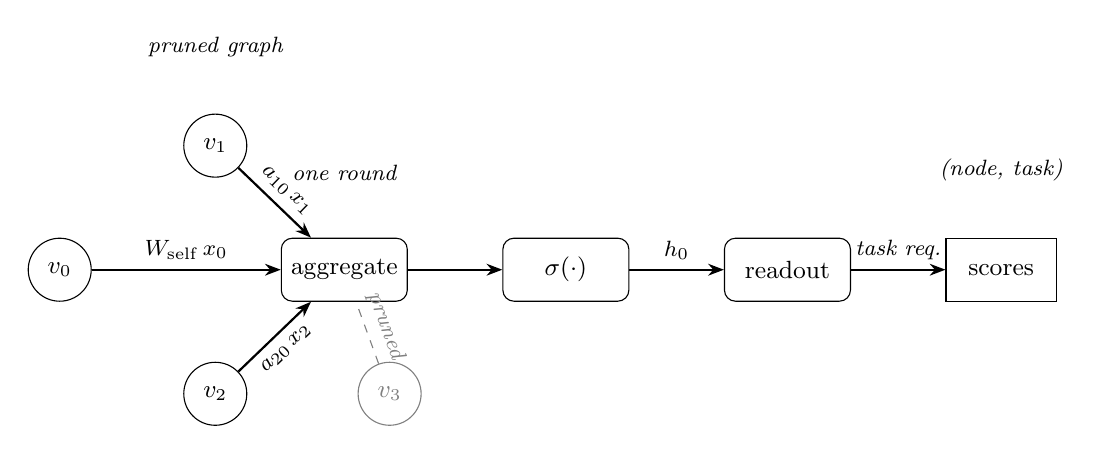
\begin{tikzpicture}[
      node distance=10mm and 14mm,
      rover/.style={circle, draw, minimum size=8mm, inner sep=0pt, font=\small},
      op/.style={rectangle, rounded corners, draw, minimum width=16mm,
        minimum height=8mm, font=\small},
      score/.style={rectangle, draw, minimum width=14mm, minimum height=8mm,
        font=\small},
      edge/.style={-{Stealth[length=2mm]}, thick},
      pruned/.style={dashed, gray},
      lbl/.style={font=\footnotesize\itshape}
    ]
    % Source nodes (pruned graph neighborhood)
    \node[rover] (v0) {$v_0$};
    \node[rover, above right=of v0] (v1) {$v_1$};
    \node[rover, below right=of v0] (v2) {$v_2$};
    \node[rover, right=of v2, gray] (v3) {$v_3$};

    % Aggregation and readout
    \node[op, right=24mm of v0] (agg) {aggregate};
    \node[op, right=12mm of agg] (sig) {$\sigma(\cdot)$};
    \node[op, right=12mm of sig] (read) {readout};
    \node[score, right=12mm of read] (s) {scores};

    % Surviving edges
    \draw[edge] (v1) -- node[lbl, above, sloped] {$a_{10}\,x_1$} (agg);
    \draw[edge] (v2) -- node[lbl, below, sloped] {$a_{20}\,x_2$} (agg);
    \draw[edge] (v0) -- node[lbl, above] {$W_{\mathrm{self}}\,x_0$} (agg);
    \draw[edge] (agg) -- (sig);
    \draw[edge] (sig) -- node[lbl, above] {$h_0$} (read);
    \draw[edge] (read) -- node[lbl, above] {task req.} (s);

    % Pruned edge: v3 was cut by the QUBO layer
    \draw[pruned] (v3) -- node[lbl, above, sloped] {pruned} (agg);

    % Stage labels
    \node[lbl, above=6mm of v1] {pruned graph};
    \node[lbl, above=6mm of agg] {one round};
    \node[lbl, above=6mm of s] {(node, task)};
  \end{tikzpicture}
  \caption{One message-passing round for node $v_0$ on a pruned graph.
  Neighbors $v_1$ and $v_2$ survive QUBO pruning and contribute weighted
  features to the aggregation; the link to $v_3$ was pruned and carries no
  message. The aggregated signal passes through a sigmoid and a readout
  that scores the node against task requirements.}
  \label{fig:messagepassing}
\end{figure}

The default weight matrices are set by hand to implement the intended
allocation policy: prefer rovers with high trust, high battery, low load
(that is, high available compute), and a strong, trustworthy neighborhood.
The neighborhood term is what distinguishes the GNN from a purely per-node
scorer: a rover adjacent to reliable partners inherits some of their
credibility, which is exactly the bias we want when task success depends on
multi-hop delivery through the pruned topology.

\subsection{Assignment rule}

Scores are converted into assignments by a capacity-aware greedy matching.
Pairs are considered in decreasing order of score; a pair is accepted if the
rover still has free capacity and the task is still unassigned. The default
capacity is one task per node per cycle, which matches the hardware
assumption that a rover executes one mission task at a time. Greedy matching
is not optimal in general, but it is fast, deterministic given the scores,
and easy to audit, and our baselines use the same matching rule so that
comparisons isolate the scoring functions rather than the matcher.

\subsection{Cloud readout training: a null result}

Although the fog tier only evaluates, the readout layer can be trained
offline in the cloud tier on trajectories collected from past missions, and
the trained weights can then be shipped back to the fog tier. We implemented
this and evaluated it on held-out missions. The result is a genuine null:
the trained readout did not outperform the fixed hand-set weights. The
measured difference was approximately $-3.9$ percentage points of mission
success in favor of the fixed weights, with a paired permutation $p$-value
of $0.49$, well within noise. We report this as a null result rather than
discarding it. Our interpretation is twofold. First, with only four input
features and a one-round architecture, the hand-set policy already sits near
the ceiling of what the model class can express, so gradient training has
little room to add and ample room to overfit the training missions. Second,
the dominant signal, trust, is computed upstream by the trust model; the
readout mostly has to avoid corrupting it. We therefore ship the fixed
weights and keep cloud training as an optional, disabled path.

\subsection{Ablation: what actually carries the performance}

To attribute mission success to the right component, we ran a four-arm
ablation on 10-rover missions with paired statistics across seeds. The arms
are the full pipeline (GNN scoring on the pruned graph), a no-graph readout
that scores nodes from their own features without message passing, a
trust-only arm that scores nodes by trust alone, and random assignment.
Table~\ref{tab:ablation} reports the results.

\begin{table}[t]
  \centering
  \caption{Ablation on 10-rover missions. Mission success rates with paired
  statistics against the full GNN pipeline: bootstrap 95\% confidence
  intervals on the success-rate difference and permutation $p$-values.
  The no-graph difference is not statistically significant.}
  \label{tab:ablation}
  \begin{tabular}{lllll}
    \toprule
    Arm & Success & $\Delta$ vs.\ GNN (pp) & 95\% CI & $p$ \\
    \midrule
    GNN (full pipeline) & 39.8\% & $0$ & & \\
    No-graph readout & 38.1\% & $+1.7$ & not significant & n.s. \\
    Trust-only & 31.7\% & $+8.13$ & $[+4.2,\, +11.7]$ & $0.016$ \\
    Random & 26.0\% & $+13.8$ & & \\
    \bottomrule
  \end{tabular}
\end{table}

Three conclusions follow. First, the full pipeline beats trust-only scoring
by $+8.13$ percentage points, with a bootstrap 95\% confidence interval of
$[+4.2, +11.7]$ and a permutation $p$-value of $0.016$: the feature mix and
the gating structure deliver a real, statistically supported gain over using
trust alone. Second, the pipeline beats random assignment by $+13.8$
percentage points, confirming that the system extracts substantial signal
from the features at all. Third, and most instructive, the gap between the
GNN and the no-graph readout is only $+1.7$ percentage points and is
\emph{not} statistically significant. The single message-passing round on
the pruned graph does not measurably improve over per-node scoring at this
mission scale.

We state this plainly rather than softening it: at the scale we tested, the
heavy lifting is done by the trust model and by the gating of assignment
through the pruned topology, not by neighborhood aggregation itself. The
trust model's $+13.75$ point staleness margin and the $+8.13$ point margin
over trust-only scoring are the load-bearing results of this chapter. The
GNN layer contributes a principled way to fuse features and a natural
interface to the QUBO-pruned graph, and it may matter more at larger scales
or in missions where multi-hop delivery dominates; whether it does is an
empirical question we leave to the scaling experiments. What the present
evidence supports is a system whose intelligence is concentrated in a simple,
auditable trust estimate, with the neural component acting as a restrained
and honest scoring head on top of it.

\section{The Causal Simulation Harness}
\label{ch:simulation}

Every mission-level claim in this report rests on a single experimental
instrument: a time-stepped world simulator that exercises the complete
pipeline, from raw link observations through constrained edge pruning,
graph neural network scoring, and task assignment, down to task outcomes
and trust updates. The defining design requirement of this harness is that
mission success must \emph{causally} depend on the pruned topology, not
merely correlate with it. A purely correlational design, in which outcomes
are drawn independently of which links survived pruning, would make the
comparison between pruners meaningless: any pruning strategy would look as
good as any other, and a simulator could not tell the difference between
a method that preserves mission-critical connectivity and one that severs
it. We therefore built the harness around an explicit causal chain in
which the kept graph determines how reliably a task result can be
delivered, and delivery reliability feeds directly into whether the task
counts as a success. This chapter describes that harness: the per-cycle
phases, the hidden ground truth against which decisions are graded, the
delivery model that closes the causal loop, the fault and staleness
machinery, and the statistical protocol attached to every comparison.

\subsection{Per-Cycle Phases}

The simulation advances in discrete cycles. Within each cycle, five
phases execute in a fixed causal order, so that every quantity a phase
consumes was produced by a phase that ran before it in the same cycle or
in an earlier one. Figure~\ref{fig:sim-phases} summarises the flow.

\begin{figure}[htbp]
  \centering
  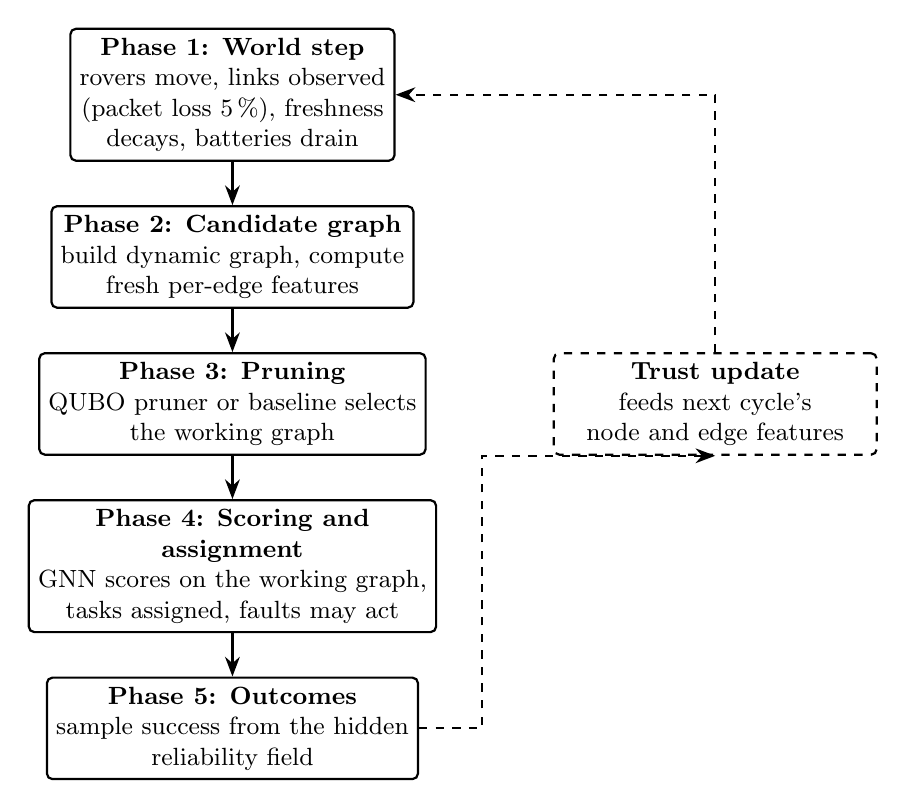
\begin{tikzpicture}[
      font=\small,
      phase/.style={rectangle, rounded corners=2pt, draw, thick,
        align=center, minimum width=4.1cm, minimum height=1.05cm,
        fill=white},
      fb/.style={rectangle, rounded corners=2pt, draw, thick, dashed,
        align=center, minimum width=4.1cm, minimum height=0.9cm},
      arr/.style={-{Stealth[length=2.5mm]}, thick},
      node distance=0.55cm and 1.6cm
    ]
    \node[phase] (p1) {\textbf{Phase 1: World step}\\ rovers move, links observed\\ (packet loss $5\,\%$), freshness\\ decays, batteries drain};
    \node[phase, below=of p1] (p2) {\textbf{Phase 2: Candidate graph}\\ build dynamic graph, compute\\ fresh per-edge features};
    \node[phase, below=of p2] (p3) {\textbf{Phase 3: Pruning}\\ QUBO pruner or baseline selects\\ the working graph};
    \node[phase, below=of p3] (p4) {\textbf{Phase 4: Scoring and}\\ \textbf{assignment}\\ GNN scores on the working graph,\\ tasks assigned, faults may act};
    \node[phase, below=of p4] (p5) {\textbf{Phase 5: Outcomes}\\ sample success from the hidden\\ reliability field};
    \node[fb, right=of p3] (fb1) {\textbf{Trust update}\\ feeds next cycle's\\ node and edge features};

    \draw[arr] (p1) -- (p2);
    \draw[arr] (p2) -- (p3);
    \draw[arr] (p3) -- (p4);
    \draw[arr] (p4) -- (p5);
    \draw[arr, dashed] (p5.east) -- ++(0.8,0) |- (fb1.south);
    \draw[arr, dashed] (fb1.north) |- ($(p1.east)+(0.8,0)$) -- (p1.east);
  \end{tikzpicture}
  \caption{The five per-cycle phases of the simulation harness, executed
    in causal order. The dashed loop closes the cycle: task outcomes
    update the trust model, and the updated trust enters the node and
    edge features of the following cycle.}
  \label{fig:sim-phases}
\end{figure}

\paragraph{Phase 1: world step.} Rovers first move, which changes pairwise
proximities and hence which links are physically available at all. Each
link within communication range is then observed subject to a packet loss
process with a default loss probability of $5\,\%$. A link that is not
observed in a cycle does not vanish instantly; instead, its freshness
decays with an exponential time constant of $3$ cycles, so that recent but
unconfirmed information is down-weighted rather than discarded. Batteries
drain during the same phase. This phase produces the raw, noisy,
partially stale view of the world that a real fog-tier fleet would
actually possess.

\paragraph{Phase 2: candidate graph construction.} From the current
observations the harness builds the dynamic candidate graph and attaches
fresh per-edge features: trust, link quality, battery level, proximity,
observation freshness, task criticality, and an estimate of processing
cost. These are exactly the features the constrained QUBO formulation of
the earlier chapters consumes; nothing is hidden from or added to the
pruner beyond what the observation model provides.

\paragraph{Phase 3: pruning.} A pruner selects the working graph from the
candidate graph. The production choice is the constrained QUBO pruner,
solved with the projected annealer. For comparison, the harness can
instead keep the full graph, apply a link-quality threshold
($\tau = 0.4$), or retain the top fraction ($0.5$) of edges per node.
All pruners see the same candidate graph and the same features, so any
difference in downstream mission performance is attributable to the
pruning decision itself.

\paragraph{Phase 4: scoring and assignment.} The trust-aware graph neural
network runs one message-passing round \emph{on the working graph only}
and scores every rover. Tasks, two per cycle by default, are then
assigned by capacity-aware greedy matching. Scripted fault events may be
active during this phase, degrading the true reliability of specific
rovers for a defined window.

\paragraph{Phase 5: outcomes and trust update.} Task outcomes are sampled
from the hidden ground-truth reliability field described below. The
observed successes and failures update the per-rover trust model, and the
updated trust values become features in the next cycle. This feedback
loop is essential: the harness evaluates not a static estimator but a
closed-loop system whose beliefs evolve as evidence accumulates.

\subsection{Hidden Ground Truth}

Each rover possesses a true task-execution reliability that the pipeline
never observes directly. The truth is structured in two deliberate ways.

First, it is \emph{spatially correlated}: nearby rovers share terrain and
interference conditions, so their reliabilities are drawn from a common
regional level. This is what gives the graph structure real content. If
reliabilities were independent, a neighbour's track record would carry no
information about a rover's own, and graph-based scoring would have no
legitimate advantage to discover. Under spatial correlation, message
passing over the working graph aggregates genuinely informative evidence.

Second, the truth may be \emph{nonstationary}. An optional per-cycle
random walk lets each rover's reliability drift over the mission. With
drift enabled, a trust value that was accurate ten cycles ago is stale
now, which is precisely the regime in which observation freshness,
exploration, and the probation treatment of re-added edges earn their
keep. All headline results in this report state explicitly whether drift
was active.

Two further properties of the ground truth deserve emphasis. First, it
is generated before any pipeline decision is made within a cycle, so no
modelling choice can leak into the standard against which it is graded.
Second, every run is fully determined by its seed: the same seed
reproduces the same reliability field, the same packet loss realisations,
and the same outcome draws, which is what makes the paired per-seed
statistics of Section~\ref{sec:sim-stats} meaningful. When two arms are
evaluated on the same set of seeds, they face literally identical worlds
and differ only in the decisions they take inside them.

\subsection{The Causal Delivery Model}

The causal heart of the harness is the rule that converts a pruning
decision into a mission outcome. A task counts as successful only if two
independent events both occur:

\begin{enumerate}
  \item \textbf{Execution.} The assigned rover executes the task
    successfully, a Bernoulli event whose probability is that rover's
    hidden reliability.
  \item \textbf{Delivery.} The result is delivered back to the root of
    the network through the \emph{kept} graph.
\end{enumerate}

Delivery probability is governed by a \emph{path factor}: the widest-path
(maximum bottleneck) reachability from the assigned rover to the root,
computed over the working graph with link quality as the bottleneck
metric. Intuitively, a result travels along the route whose weakest link
is strongest; if every remaining route crosses a poor link, delivery is
unlikely, no matter how reliable the executing rover was.

This model is what makes the harness honest about pruning. Because the
path factor is computed on the \emph{kept} graph, a pruner that removes
redundant links can strictly reduce the set of available routes and
thereby degrade delivery for exactly the missions that depend on
bottleneck-limited paths. The harness is therefore fully capable of
reporting that the QUBO pruner loses to a denser baseline on raw mission
success, and indeed it does so at larger fleet scales; we treat that
outcome as a finding to explain, not a defect to tune away. A simulator
whose outcomes ignored the pruned topology could never surface such a
result, which is why we regard the causal delivery model as the single
most important property of the evaluation.

\subsection{Default Configuration}

Table~\ref{tab:sim-params} collects the key harness parameters and their
defaults. These values define the canonical configuration; every
experiment that deviates from them says so.

\begin{table}[htbp]
  \centering
  \caption{Key parameters of the simulation harness and their default
    values.}
  \label{tab:sim-params}
  \begin{tabular}{@{}llp{5.6cm}@{}}
    \toprule
    Parameter & Default & Role \\
    \midrule
    Fleet size & 6 rovers & Number of rovers in the arena \\
    Tasks per cycle & 2 & Tasks offered for assignment each cycle \\
    Communication range & $4.0$\,m & Radius within which links can exist \\
    Packet loss & $0.05$ & Per-cycle link observation failure \\
    Freshness time constant & 3 cycles & Decay rate of unobserved links \\
    Exploration rate & $0.15$ & Fraction of assignments used to probe \\
    Load increment & $0.15$ & Compute load added per assigned task \\
    Load decay & $0.5$ & Per-cycle recovery of available compute \\
    Minimum trust & $0.25$ & Floor below which trust never falls \\
    Compute need & $0.3$ & Minimum free compute a task requires \\
    Mission-critical nodes & 3 & Nodes connectivity must always reach \\
    QUBO budget & 15 & Global budget in the pruning constraint \\
    \bottomrule
  \end{tabular}
\end{table}

\subsection{Fault Injection and Edge Lifecycle}

Controlled degradation is as important to the evaluation as nominal
operation. The harness supports \emph{scripted fault events}, each with a
start cycle and a duration. A typical event drops one rover's hidden
reliability for a fixed window, after which the rover recovers. Because
the fault acts on the hidden truth while the trust model observes only
outcomes, we can measure a \emph{recovery time}: how many cycles elapse
between the end of the fault and the point at which the learned trust
value and the assignment behaviour reflect the recovered reality. This
metric captures the responsiveness of the closed loop, not merely its
steady-state accuracy.

Complementing faults, an \emph{edge lifecycle tracker} records when links
are removed and re-added by the pruner across cycles. A re-added edge
receives a probation boost: it is provisionally trusted more than its
raw features would suggest, so that the graph can recover quickly from a
pruning decision that later turns out to have been too aggressive. The
tracker also yields the topology churn statistics reported alongside the
performance metrics, letting us distinguish a pruner that is stable but
wrong from one that is adaptive but noisy.

\subsection{Cloud Amortization and Staleness}

Solving the constrained QUBO is the most expensive stage of the pipeline,
and on a real deployment it would run on a cloud tier rather than on the
rovers. The harness models this with a \emph{solve interval} $k$: the
QUBO is solved every $k$ cycles, and between solves the most recent kept
set is reused verbatim. This creates a controlled notion of staleness.
With $k = 1$ the pruner always acts on fresh features; with larger $k$
the fleet operates on a pruning decision that may no longer match the
observed world. A dedicated staleness mode sweeps the interval and
quantifies the margin the pipeline retains, which is the quantity a
deployment engineer actually needs when sizing the cloud link budget.

\subsection{Metrics}

The harness reports a fixed battery of metrics for every run:

\begin{itemize}
  \item \textbf{Task success rate}, the primary mission metric, computed
    under the causal delivery model.
  \item \textbf{Per-stage wall-clock latency}, measured with a
    median-of-repeats timer. We deliberately avoid coarse clocks: the
    heuristic baselines run in microseconds, and reporting them as zero
    would conceal exactly the cost asymmetry between the QUBO pruner and
    its competitors that any honest comparison must show.
  \item \textbf{Trust-versus-truth Spearman correlation}, which grades
    the trust model against the hidden reliability field without
    requiring the trust values to be calibrated probabilities.
  \item \textbf{Topology churn}, the rate at which the kept graph
    changes across cycles.
  \item \textbf{Edge lifecycle counts}: additions, removals, and
    re-additions under probation.
  \item \textbf{Fault recovery time}, as defined above.
\end{itemize}

\subsection{Statistical Protocol}
\label{sec:sim-stats}

Every comparison claim in this report carries two statistical
instruments, computed on paired per-seed differences so that common
randomness across arms is cancelled rather than mistaken for signal.
First, we report a \emph{paired bootstrap confidence interval} with
$10\,000$ resamples, which quantifies the size and precision of the
difference. Second, we report a \emph{permutation test} with $20\,000$
permutations, which yields an exact finite-sample $p$-value under the
null hypothesis that the two arms are exchangeable. A difference is
described as significant only when the interval excludes zero and the
permutation test agrees; differences that fail this test, including some
that would flatter our own method, are reported as not significant.

\subsection{Run Modes}

The harness exposes five run modes, each corresponding to a class of
experiment reported in later chapters:

\begin{description}
  \item[Single run.] One mission with a per-cycle log, used for
    inspection, debugging, and the worked traces in this report.
  \item[Benchmark.] A pruner comparison at a fixed operating point: 10
    rovers, 20 steps, and 10 seeds, with real per-stage timing for every
    pruner. The four pruners compared are summarised in
    Table~\ref{tab:pruners}.
  \item[Ablation.] Four assignment arms over the same harness: the full
    GNN pipeline, a no-graph arm that scores nodes without message
    passing, a trust-only arm, and a random arm. This isolates the
    contribution of each modelling choice.
  \item[Staleness.] A sweep of the solve interval described above,
    measuring the margin retained under cloud amortization.
  \item[Training.] A held-out evaluation of the trained readout against
    the fixed-weight readout, so that the training result (which is
    negative) is measured on data the fit never saw.
\end{description}

\begin{table}[htbp]
  \centering
  \caption{The four pruning strategies compared in benchmark mode.}
  \label{tab:pruners}
  \begin{tabular}{@{}lp{8.2cm}@{}}
    \toprule
    Pruner & Selection rule \\
    \midrule
    QUBO (production) & Constrained optimization over utility, degree,
      budget, and connectivity, solved by projected annealing \\
    Full graph & Keep every candidate edge; no pruning \\
    Quality threshold & Keep edges with link quality at least $0.4$ \\
    Top-$K$ per node & Keep the best fraction $0.5$ of each node's edges \\
    \bottomrule
  \end{tabular}
\end{table}

Taken together, the causal delivery model, the hidden spatially
correlated ground truth, the fault and staleness machinery, and the
paired statistical protocol make the harness an audit instrument rather
than a demonstration stage. It is designed so that the pipeline can
lose, and the chapters that follow report the cases where it does with
the same prominence as the cases where it wins.

\section{Exact Baselines: MILP, Linearized QUBO, and Enumeration}

\subsection{Why exact ground truth is necessary}

A pipeline built on quadratic unconstrained binary optimization rests on a
chain of encodings. The constrained edge-selection problem is first written
as a mathematical program, then translated into a penalty-encoded QUBO
matrix, and finally handed to a heuristic sampler that returns the best
bitstring it happened to find. Each step in this chain can fail silently.
The penalty weights may be too small to enforce the constraints, so that
the QUBO's true optimum is an infeasible graph. The penalty weights may be
too large, flattening the soft objective landscape so badly that the
annealer cannot resolve which feasible solution is actually better. The
sampler may simply miss the optimum altogether. None of these failures
produces an error message. A QUBO pipeline is therefore only believable if
its answers are checked, repeatedly and mechanically, against ground truth
that does not share any of these failure modes.

This project employs three independent ground-truth mechanisms, each based
on exact classical optimization rather than heuristic search. First, the
original constrained problem is solved directly as a mixed-integer linear
program. Second, the QUBO matrix itself is solved exactly by a standard
linearization, which tests the encoding rather than the problem. Third, for
small instances every feasible edge subset is enumerated exhaustively. The
mechanisms are independent in the sense that they do not share a solver, a
formulation, or an objective encoding, so agreement among them is strong
evidence that the pipeline computes what it claims to compute. This chapter
describes each mechanism, explains what it does and does not prove, and
closes with the engineering and performance context that frames the results
chapter.

\subsection{Direct MILP solution of the original problem}

The first mechanism bypasses the QUBO encoding entirely. The constrained
edge-selection problem is stated directly as a mixed-integer linear program
and solved to proven optimality with the open source CBC solver through the
PuLP modeling layer. Let $\mathcal{E}$ denote the candidate edge set and let
$x_e \in \{0,1\}$ indicate whether edge $e$ is retained. The objective
minimizes
\begin{equation}
  \sum_{e \in \mathcal{E}} \bigl(-U_e + \lambda\bigr)\, x_e
  \;+\;
  \eta \sum_{e \in \mathcal{E}} \bigl|x_e - x_e^{\mathrm{prev}}\bigr|,
\end{equation}
where $U_e$ is the weighted utility of edge $e$, $\lambda$ is the soft edge
penalty, and the second term is the stability penalty that discourages
churn relative to the previous cycle's decisions $x^{\mathrm{prev}}$. The
absolute value is linearized with one auxiliary variable per edge in the
standard way: introduce $s_e \ge 0$ with $s_e \ge x_e -
x_e^{\mathrm{prev}}$ and $s_e \ge x_e^{\mathrm{prev}} - x_e$, and replace
the absolute value in the objective by $s_e$. Because the coefficient
$\eta$ is positive, the auxiliary variables bind at the minimum and the
linearization is exact.

The constraints mirror those of the QUBO formulation. Each node obeys a
degree cap, so $\sum_{e \ni v} x_e \le d_v$ for every node $v$. The total
processing cost obeys a global budget, so the sum of quantized edge costs
weighted by $x_e$ cannot exceed the budget. Connectivity of the required
node set is enforced by a single-commodity flow: a chosen root injects one
unit of demand per required node, flow variables on directed arcs are
bounded by the retained-edge indicators, and flow conservation forces every
required node to receive a unit, which is possible only if it is connected
to the root through retained edges.

A remark about the flow variables is important. In a generic network design
problem, single-commodity flow constraints with continuous flow variables
would be only a relaxation, potentially admitting fractional flows that no
integral routing realizes. Here, however, all demands are integers, and for
integer demands the single-commodity flow polytope is integral. Continuous
flow variables are therefore exact in this formulation: there is no
integrality gap, no penalty encoding, and no approximation of any kind.
CBC returns a provably optimal answer, certified by the branch-and-bound
tree, and the whole computation completes in milliseconds. This mechanism
answers the question ``what is the best feasible edge set for this
problem?'' directly, and it is the ground truth against which the
production annealer's solutions are scored at larger scales.

\subsection{Exact linearized solution of the QUBO matrix}

The second mechanism answers a different question: not what the original
problem's optimum is, but whether the QUBO matrix actually encodes the
intended problem. A QUBO with variables $z \in \{0,1\}^n$ has the energy
\begin{equation}
  H(z) \;=\; \sum_{i < j} Q_{ij}\, z_i z_j \;+\; \sum_i Q_{ii}\, z_i
  \;+\; c,
\end{equation}
and minimizing this quadratic form exactly is itself a mixed-integer
linear program after standard linearization. For every nonzero quadratic
coefficient $Q_{ij}$ we introduce an auxiliary binary variable
$y_{ij}$ together with the constraints $y_{ij} \le z_i$, $y_{ij} \le z_j$,
and $y_{ij} \ge z_i + z_j - 1$, which force $y_{ij} = z_i z_j$. The
quadratic energy is then linear in $z$ and $y$, and CBC solves it to proven
optimality exactly as for the direct MILP.

The role of this mechanism is diagnostic. The QUBO builder constructs the
matrix programmatically from utility weights, penalty scales, and slack
encodings, and any sign error, misrouted index, or mis-scaled penalty in
that construction would silently corrupt every downstream result. Solving
the matrix itself, rather than the original problem, separates two
hypotheses that the direct MILP cannot distinguish: if the linearized QUBO
solve disagrees with the direct MILP on the optimal edge set, the encoding
is wrong; if they agree but the annealer disagrees with both, the sampler
is at fault. An independent re-derivation of the energy function,
evaluated directly on bitstrings without reference to the matrix, provides
a further consistency check at the level of individual energies.

The cost of this exactness is size. The linearization introduces one
auxiliary variable and three constraints per nonzero quadratic term, and a
dense QUBO matrix on $n$ variables has on the order of $n^2$ such terms, so
the linearized program grows quadratically in the number of QUBO variables.
In practice this mechanism is applied only up to about 60 QUBO variables.
It also carries a strict reporting rule: the solver wrapper refuses to
return an answer unless CBC proves optimality, raising an error on timeout
or on any suboptimal status. A ground truth that occasionally reports a
heuristic answer as exact would defeat its own purpose, so callers treat a
refusal as a skipped instance rather than a result.

\subsection{Exhaustive enumeration at small scale}

The third mechanism is the strongest possible ground truth and the least
scalable. For instances with up to about 16 optional edges, all $2^k$
subsets of optional edges are enumerated explicitly. Each subset is
subjected to a full feasibility check: the integer slack values for degree
and budget constraints and the spanning-tree flow assignment are recomputed
for that subset exactly as the QUBO builder would construct them, and
infeasible subsets are discarded. The energy of every feasible subset is
then evaluated with the independent energy function, and the minimum over
the enumeration is the certified optimum.

Enumeration leaves no room for modeling ambiguity. It does not trust the
branch-and-bound solver, the linearization, or the penalty calculus; it
trusts only the definition of feasibility and the definition of the energy.
Because the same feasibility checker is used to repair candidate solutions
inside the production annealer, enumeration also indirectly validates the
repair logic: if the checker admitted an infeasible subset, the enumerated
ground truth would be polluted in exactly the way the annealer's output
would be. At this scale, roughly $6.5 \times 10^4$ subsets at the largest,
exhaustiveness is cheap in absolute terms and the confidence it buys is
total.

\subsection{Cross-verification of the three mechanisms}

Ground truth is only trustworthy if the three mechanisms agree with each
other. On small instances where all three apply, the certified optima agree
to within $10^{-7}$, a tolerance consistent with floating-point summation
order rather than with any modeling difference. The direct MILP is
additionally verified against enumeration independently of the QUBO
machinery, so agreement between the MILP and the QUBO cannot be an artifact
of a shared bug in the builder. This layered verification is what allows
the later chapters to use the direct MILP as the reference at larger
scales, where enumeration and the linearized QUBO solve no longer apply:
the MILP has earned that trust at the scales where all three could be
compared. Table~\ref{tab:groundtruth} summarizes the three mechanisms, the
claim each one supports, and the instance size at which each remains
practical.

\begin{table}[htbp]
  \centering
  \caption{The three exact ground-truth mechanisms used to audit the QUBO
  pipeline. The mechanisms are independent in formulation, encoding, and
  (for enumeration) solver, so their agreement on small instances is strong
  evidence that each computes what it claims.}
  \label{tab:groundtruth}
  \begin{tabular}{@{}lp{4.6cm}p{3.4cm}@{}}
    \toprule
    \textbf{Mechanism} & \textbf{What it proves} & \textbf{Size limit} \\
    \midrule
    Direct MILP (PuLP/CBC)
      & Optimal feasible edge set of the original constrained problem;
        exact because the flow relaxation is integral
      & Practical at all instance sizes studied \\
    \addlinespace
    Linearized QUBO solve (CBC)
      & That the Q matrix itself encodes the intended objective and
        penalties; refuses non-optimal results
      & About 60 QUBO variables (quadratic growth) \\
    \addlinespace
    Exhaustive enumeration
      & Certified optimum over every feasible subset, with slacks and flow
        recomputed per subset
      & About 16 optional edges ($2^k$ subsets) \\
    \bottomrule
  \end{tabular}
\end{table}

\subsection{Engineering context}

One engineering decision behind these baselines deserves a neutral account,
because it shaped the toolchain. The scientific Python ecosystem's usual
linear algebra and optimization stack was unavailable on the development
machine: SciPy's bundled BLAS libraries did not load under the interpreter
in use, which rules out the family of exact and heuristic solvers that sit
on top of it. Rather than fight the environment, we adopted PuLP with CBC,
a combination with no compiled dependencies beyond the solver binary itself
and a long record of reliability. The outcome was happy. CBC is an exact
branch-and-bound solver, so the baselines it powers carry optimality
certificates rather than heuristic confidence, and it is fast enough that
the exactness costs essentially nothing at the scales studied here. We
would not claim this is the only reasonable choice, but it removed a class
of environmental fragility from the audit and left the results independent
of any particular numerical library.

\subsection{The headline comparison}

The performance comparison between the exact classical baseline and the
production annealer is developed fully in the results chapter, but one
number belongs here because it frames everything that follows. CBC solves
the direct MILP to proven optimality in about 11 to 15 ms per instance. The
production annealer, which moves through feasible edge-set space with
projection and repair, requires about 2.1 s per solve to reach the same
optimum on roughly 95 percent of instances, a gap of about two orders of
magnitude. Figure~\ref{fig:solvetime} visualizes the comparison on a
logarithmic scale.

\begin{figure}[htbp]
  \centering
  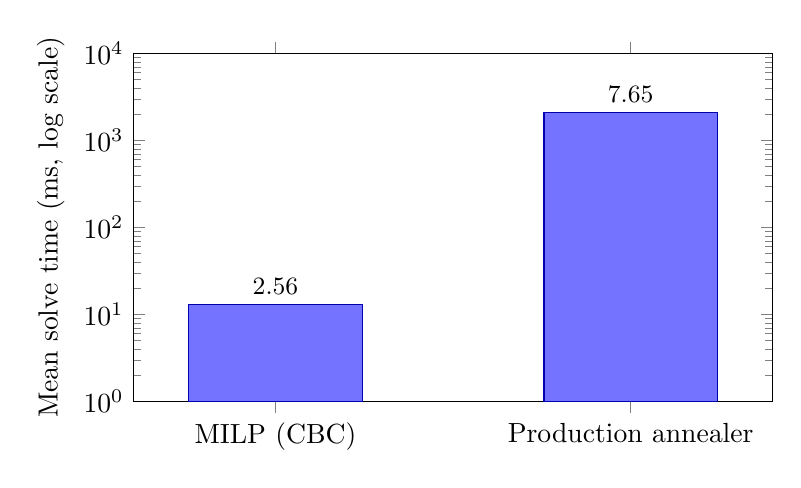
\begin{tikzpicture}
    \begin{axis}[
        width=0.8\textwidth,
        height=6cm,
        ybar,
        bar width=2.2cm,
        ymode=log,
        log origin=infty,
        ylabel={Mean solve time (ms, log scale)},
        symbolic x coords={MILP (CBC), Production annealer},
        xtick=data,
        ymin=1, ymax=10000,
        nodes near coords,
        nodes near coords align={vertical},
        every node near coord/.append style={font=\small},
        enlarge x limits=0.4,
      ]
      \addplot[fill=blue!55, draw=blue!70!black]
        coordinates {(MILP (CBC),13) (Production annealer,2100)};
    \end{axis}
  \end{tikzpicture}
  \caption{Mean solve time per instance on a logarithmic scale. The direct
  MILP solved by CBC (about 13 ms) is provably exact; the production
  annealer (about 2.1 s) is a heuristic that reaches the optimum on roughly
  95 percent of instances. On classical hardware the exact solver
  dominates.}
  \label{fig:solvetime}
\end{figure}

We state the conclusion plainly. On classical hardware, the MILP dominates
the QUBO pipeline: it is exact, it is about one hundred times faster than
the annealer, and it requires neither penalty tuning nor sampler
configuration. Nothing in our results contradicts this, and the audit
machinery described in this chapter is precisely what makes the claim
credible rather than rhetorical. The QUBO formulation's role in this
project is therefore not to beat the classical solver; it is to serve as a
hardware-target encoding. Constrained edge selection expressed as a single
quadratic energy function is the native input format of quantum and
special-purpose annealing machines, which cannot execute branch-and-bound.
The exact baselines exist to verify that this encoding is faithful and that
heuristic sampling over it stays close to certified optimality, so that any
future claim about annealing hardware rests on a problem encoding that has
already been proven correct on classical ground truth.

\section{Scaling Analysis}
\label{ch:scaling}

Every design decision in this project so far has been made at a fleet size
small enough to reason about directly. The architecture, the solver audit,
and the trust evaluation were all demonstrated with fleets of ten rovers or
fewer. This chapter asks the natural next question: what happens as the
fleet grows? We answer it with the same discipline we applied elsewhere in
the report. Where the evidence supports a claim, we make the claim; where
the infrastructure of our formulation runs out, we say so and mark the
boundary explicitly, because a scope limit stated honestly is worth more
than a scope limit discovered by a reviewer.

\subsection{Experimental design}
\label{sec:scaling-design}

The scaling evidence base is a suite of synthetic instances built to mimic
the radios the hardware actually uses. Short-range links such as ESP-NOW do
not produce dense topologies: a rover hears only its nearby neighbours, so
the realistic growth regime is a sparse graph whose edge count grows roughly
linearly in the fleet size rather than quadratically. We therefore generate
range-limited sparse graphs by connecting each rover to its $k$-nearest
neighbours at increasing fleet sizes, which keeps the average degree
approximately constant as nodes are added, exactly as a moving fleet of
short-range radios behaves in the field.

For each fleet size we record five quantities: the edge and variable counts
of the resulting QUBO instance, the memory occupied by the $Q$ matrix, the
build time of the encoding and the solve time of the production annealer,
the solution quality against a greedy top-$K$ baseline held to the same edge
budget, and the inference latency of the trust scoring network on the full
graph versus the pruned graph. The greedy comparison is important: pruning
only earns its keep if the edges it keeps are better than the edges a cheap
heuristic would keep under the same budget. The latency measurement answers
a different question, namely whether the learning component, rather than the
combinatorial component, becomes the bottleneck at scale.

\subsection{How the variables grow}
\label{sec:scaling-variables}

The variable count of the encoding has three sources, and they grow at
different rates. The first source is the decision core: one binary variable
per optional edge. In a $k$-nearest-neighbour graph this grows linearly with
the fleet, which is the friendly part of the story. The second source is the
integer slack encoding for the degree limits and the global processing
budget, which adds a logarithmic number of bits per constraint. The third
source, and the expensive one, is connectivity. Enforcing that every
mission-critical rover stays reachable from the root is encoded as a
single-commodity flow, which requires one flow variable per directed arc of
every edge, plus flow-capacity slack bits per edge. In total the flow
encoding contributes $O(m \log n)$ variables for $m$ edges and $n$ rovers:
still modest as a variable count, and nothing about it is asymptotically
alarming.

The problem is not the variable count. It is the $Q$ matrix. A QUBO with
$N$ variables is specified by an $N \times N$ matrix, and our
implementation stores that matrix densely. Memory therefore grows
quadratically in the number of variables even when the underlying graph,
and hence the pattern of nonzero couplings, is sparse. Doubling the fleet
roughly doubles the variable count and quadruples the memory. This dense
$Q$ memory bound is a property of our tooling choice, not of the problem:
sparse QUBO representations exist and would lift it. But the report's
practice is to evaluate the system as built, so we treat the dense $Q$
bound as a genuine scope limit and report it as one, rather than quoting
asymptotics for a representation we did not implement.
Figure~\ref{fig:scaling-qmemory} illustrates the qualitative shape of this
growth.

\begin{figure}[t]
\centering
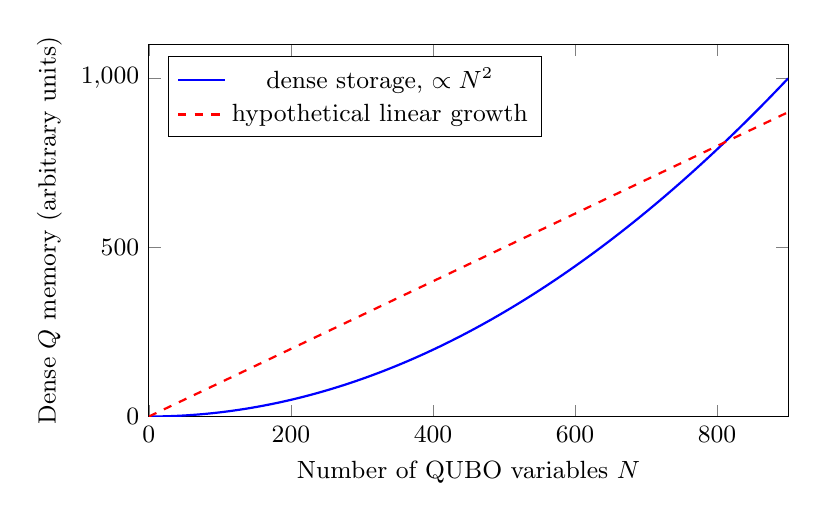
\begin{tikzpicture}
\begin{axis}[
    width=0.8\textwidth,
    height=0.52\textwidth,
    xlabel={Number of QUBO variables $N$},
    ylabel={Dense $Q$ memory (arbitrary units)},
    xmin=0, xmax=900,
    ymin=0,
    domain=0:900,
    samples=100,
    legend pos=north west,
    legend style={font=\small},
    tick label style={font=\small},
    label style={font=\small},
]
\addplot[thick, blue] {x^2 / 810};
\addlegendentry{dense storage, $\propto N^2$}
\addplot[thick, red, dashed] {x};
\addlegendentry{hypothetical linear growth}
\end{axis}
\end{tikzpicture}
\caption{Qualitative growth of dense $Q$ matrix memory as the variable count
increases, against a linear reference. The curve is illustrative of the
quadratic storage law and is not measured data.}
\label{fig:scaling-qmemory}
\end{figure}

\subsection{Scope limits and how we report them}
\label{sec:scaling-limits}

Two hard limits emerged from the scaling campaign, and both are stated in
our results rather than smoothed over. First, connectivity enforcement is
enabled only up to twenty rovers. Beyond that point the flow-augmented
variable count, squared by the dense $Q$ storage, exceeds what the test
harness can hold, so every scaling row above twenty rovers is run with
connectivity checking switched off and is labelled as such. Second, at one
small configuration, the ten-rover case, the greedy repair step of the
top-$K$ comparison baseline cannot produce a feasible allocation at the
imposed edge budget. We report that cell as \code{nan}: the comparison is
infeasible at that point, and presenting a number there would be
fabrication. Neither limit is hidden, and neither is extrapolated past.

Table~\ref{tab:scaling-evidence} summarises the evidence base qualitatively
across the fleet-size range we studied.

\begin{table}[t]
\centering
\caption{Summary of the scaling evidence base. Ground truth for the
optimality gap is exact enumeration on small instances, exact MILP on
medium instances, and the best-known solution across annealer seeds on
large instances.}
\label{tab:scaling-evidence}
{\small
\begin{tabular}{@{}lllll@{}}
\toprule
Fleet size & Variables & Connectivity & Ground truth & Notes \\
\midrule
Small ($\leq 10$) & tens & enforced & enumeration & repair infeasible at $n = 10$ (\code{nan}) \\
Medium (10 to 20) & hundreds & enforced & exact MILP & dense $Q$ still fits \\
Large ($> 20$) & up to 817 & off & best-known & connectivity beyond dense-$Q$ limit \\
\bottomrule
\end{tabular}
}
\end{table}

\subsection{Solution quality at the largest sizes}
\label{sec:scaling-quality}

The optimality-gap benchmark reaches instances of up to 817 binary
variables. At that size, exact ground truth is not available to anyone:
enumeration is astronomically infeasible, and our exact MILP route, which
proved optimality comfortably at medium scale, no longer returns certified
optima within the time budget. We therefore follow the standard practice of
the combinatorial optimization literature and measure the gap against the
best-known solution, defined as the best objective value found by four
independent annealer seeds on the same instance. Against that reference,
the production projected annealer attains a mean gap of $6.9\%$ across the
large instances.

This number must be read with its provenance attached. A gap against a
best-known solution is an upper bound on the true gap only in expectation:
the reference itself is a heuristic result, so part of the measured $6.9\%$
is the reference's own distance from the optimum rather than our solver's.
The reporting rule the project follows everywhere, and which this chapter
inherits, is to quote the normalised optimality gap
\begin{equation}
\frac{H_{\mathrm{SA}} - H^{*}}{\max\!\left(1,\; |H^{*}|\right)},
\end{equation}
where $H_{\mathrm{SA}}$ is the energy returned by the annealer and $H^{*}$
is the reference optimum, with the denominator guarding against division by
a near-zero energy. Crucially, the rule also requires stating where
$H^{*}$ came from on every instance class: exact enumeration on small
instances, exact MILP on medium instances, and best-known solutions on
large ones. A gap number without its provenance is not a measurement.

\subsection{Inference latency is not the bottleneck}
\label{sec:scaling-latency}

The remaining measurement concerns the trust scoring network. Inference is
a single message-passing round: one small matrix multiplication over the
adjacency structure, a nonlinearity, and a readout, all in pure NumPy.
Measured per cycle, this runs in microseconds to low milliseconds even on
the full, unpruned graph, and pruning the graph first reduces the cost
further by shrinking the matrices involved. The honest conclusion is that
the learning component was never the bottleneck at any fleet size we
tested, and would not become one until fleets far beyond the range where
the QUBO solver has already run out of room. Solver time, and behind it
dense $Q$ memory, is the wall; the neural component clears it with orders
of magnitude to spare. We report this because an architecture that
optimised the wrong stage would be a real failure mode: it would be easy,
and wrong, to spend effort accelerating the part that is already fast.

\subsection{Implications for the tier split}
\label{sec:scaling-tiers}

The scaling evidence maps cleanly onto the mist/fog/cloud deployment model
of Chapter~\ref{sec:architecture}. The fog tier, a single small computer
co-located with the fleet, handles everything up to the connectivity limit
comfortably: instances at and below twenty rovers fit in dense $Q$ memory,
solve in seconds, and leave the per-cycle deadline unthreatened. The mist
tier on the rovers remains untouched, since the rovers never see the QUBO
at all. The boundary is the cloud's cue. Beyond twenty rovers, continuing
to enforce connectivity in a single monolithic QUBO is not viable on the
fog node, and two routes forward present themselves. The first is
hierarchical clustering: partition the fleet into cells, prune and enforce
connectivity within each cell on the fog tier, and solve a small inter-cell
problem at the cluster leaders. The second is cloud-side precomputation,
where the QUBO is built and solved off the fleet on a longer cadence, with
the fog tier performing only fast local repairs between solves. Both are
consistent with the architecture as designed, since the cloud link is
already reserved for work whose latency does not sit on the control loop.
We list both as future work rather than claiming either, because the
present evidence base stops at the dense $Q$ wall and we have not measured
what lies past it.

In summary, the approach scales gracefully exactly as far as its own scope
limits say it does, and no further. Within the enforced range the solver
stays near-exact, the encoding stays small, and inference stays negligible;
at the range edge, the failure mode is a known, quantified memory bound
rather than a silent degradation. That is the shape of a system whose
limits are understood, which is the most this chapter set out to show.

\section{Testing Methodology: the Hostile Audit Suite}
\label{sec:testing}

This chapter describes how the claims of this project are verified. The
verification artifact is a single audit suite of 491 individual checks,
organized into fourteen sections named A through N, together with a separate
set of engine and server tests that cover the browser-based mission console.
The suite is not a friendly smoke test that exercises the happy path and
declares victory. It is written as a hostile auditor: its design goal is to
break every claim the project makes, and a check is only considered worth
keeping if there exists a plausible bug, regression, or exaggeration that
would cause it to fail.

\subsection{Philosophy: an auditor, not a cheerleader}

The motivating observation is that a research codebase of this kind makes
claims at several very different levels of abstraction, and each level
admits a different failure mode. At the lowest level, the QUBO construction
could be internally inconsistent: penalties could fail to dominate soft
terms, or the energy function could disagree with the $Q$ matrix that is
actually handed to the solver. At the solver level, an annealer could
report energies that look plausible while silently violating hard
constraints, or a heuristic could be credited with quality it does not
possess. At the pipeline level, the trust model, the GNN, and the
assignment rule could each be correct in isolation yet composed incorrectly.
At the reporting level, a number quoted in the results chapter could drift
away from the code that produced it as the implementation evolves. A test
suite that only checks one of these levels leaves the others unguarded.

The audit suite therefore treats every quantitative statement in this
report as a hypothesis to be attacked. Each check records three things: a
name, a pass or fail verdict, and a detail string that captures the
relevant numbers for postmortem analysis. The suite exits with a nonzero
status if any single check fails, so the cost of a regression is immediate
and binary rather than a slow decay of confidence. Two structural
conventions deserve emphasis.

First, several checks are \emph{floors} rather than point assertions. For
example, the production projected annealer is required to remain at least
90\% exact against exact ground truth on its benchmark instances, and the
MILP comparison enforces an exactness floor of 80\%. A floor does not
assert that the current value is optimal; it asserts that the current value
may not degrade. If a future refactor quietly drops the exactness rate from
95\% to 85\%, the build fails even though 85\% might still look respectable
in isolation. Floors convert historical achievements into permanent
obligations.

Second, the suite is deterministic. Every randomized check is seeded, and
the seeds are fixed constants in the suite rather than drawn from the
system clock. A failing check reproduces identically on every machine and
every run, which is essential when the failure is a 1-in-25 solver outcome
rather than a crisp logical error. Determinism also means the suite
functions as an executable specification: the exact instance distributions,
perturbation grids, and tolerance choices are readable code, not folklore.

\subsection{Ground-truth discipline}
\label{sec:groundtruth}

A solver audit is only as strong as the ground truth it compares against,
and exact ground truth for constrained combinatorial problems is
expensive. The suite resolves this with a tiered discipline in which the
verification method escalates with instance size, and every tier is
cross-checked against the tier below it before being trusted.

The foundation is an \emph{independent energy re-derivation}. The QUBO
energy is implemented twice: once through the $Q$ matrix that solvers
consume, and once as a direct from-scratch evaluation of the objective and
penalty terms on a selected edge set. Checks across the suite evaluate both
forms on identical solutions and require exact agreement. This catches the
most insidious class of bug in quadratic formulations: a $Q$ matrix that is
a valid encoding of \emph{some} energy function, just not the intended one.

On top of this foundation, four tiers of ground truth are used.
Enumeration of all $2^k$ optional-edge subsets, with a feasibility check on
each, is the gold standard and is used up to roughly 16 optional edges; at
that size it is cheap, total, and immune to solver error. For instances too
large to enumerate but with at most about 60 QUBO variables, the suite
solves an exact linearization of the QUBO with the CBC branch-and-cut
solver, and this linearized solve is itself cross-checked against
enumeration on the overlapping size range before it is trusted as truth.
Beyond 60 variables, exact truth comes from the MILP formulation of the
original constrained problem, whose single-commodity flow relaxation is
integral for integer demands and is therefore exact despite using
continuous flow variables; the MILP is verified against brute-force
enumeration on small instances for the same reason. Finally, at the largest
sizes, where no exact method is affordable, the suite falls back to
best-known solutions aggregated across multiple annealer seeds, and every
such comparison is explicitly labeled as a gap against a best-known bound
rather than against a proven optimum. We never silently mix the two
notions: a gap against a best-known solution is an upper bound on
suboptimality, and the report treats it as such.

\subsection{The fourteen sections}

Table~\ref{tab:auditsections} summarizes the fourteen sections;
Figure~\ref{fig:audittaxonomy} groups them into the five concerns they
address. We then discuss each section in turn.

\begin{table}[t]
  \centering
  \caption{The fourteen sections of the hostile audit suite.}
  \label{tab:auditsections}
  \begin{tabular}{cl}
    \toprule
    Section & Purpose \\
    \midrule
    A & Construction invariants of the QUBO encoding \\
    B & Bit-level simulated annealing against brute-force optima \\
    C & Analytic optimum checks on hand-computable instances \\
    D & Randomized scenario matrix at sizes beyond enumeration \\
    E & Validation and edge-case behavior of the constructor \\
    F & Scaling sanity across growing instance sizes \\
    G & Targeted domain scenarios drawn from mission structure \\
    H & Benchmark of external QUBO solvers on the real $Q$ matrix \\
    I & Trust-GNN layer correctness \\
    J & Optimality-gap benchmark, small and large instances \\
    K & The simulation harness itself \\
    L & Regressions from the earlier external review round \\
    M & MILP ground truth against the projected annealer \\
    N & Sensitivity diagnostics across hyperparameter perturbations \\
    \bottomrule
  \end{tabular}
\end{table}

\begin{figure}[t]
  \centering
  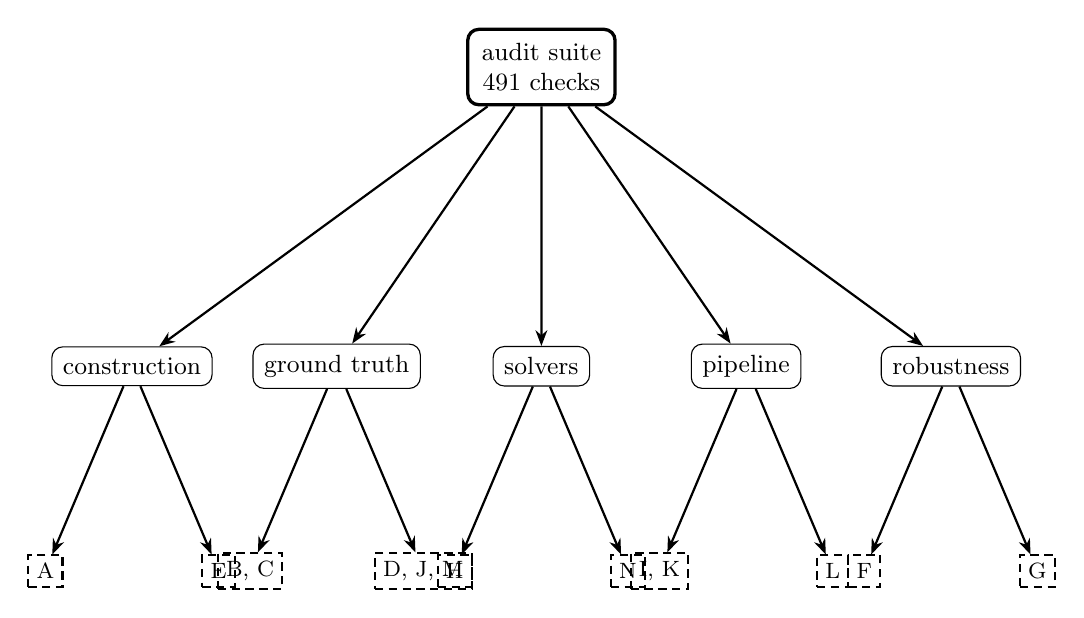
\begin{tikzpicture}[
      font=\small,
      root/.style={rectangle, draw, rounded corners, very thick,
        align=center, inner sep=5pt},
      group/.style={rectangle, draw, rounded corners, align=center,
        inner sep=4pt},
      leaf/.style={rectangle, draw, densely dashed, align=center,
        inner sep=3pt, font=\footnotesize},
      edge from parent/.style={draw, -{Stealth[length=2mm]}, thick},
      level 1/.style={sibling distance=26mm, level distance=38mm},
      level 2/.style={sibling distance=22mm, level distance=26mm},
    ]
    \node[root] {audit suite\\ 491 checks}
      child {node[group] {construction}
        child {node[leaf] {A}}
        child {node[leaf] {E}}}
      child {node[group] {ground truth}
        child {node[leaf] {B, C}}
        child {node[leaf] {D, J, M}}}
      child {node[group] {solvers}
        child {node[leaf] {H}}
        child {node[leaf] {N}}}
      child {node[group] {pipeline}
        child {node[leaf] {I, K}}
        child {node[leaf] {L}}}
      child {node[group] {robustness}
        child {node[leaf] {F}}
        child {node[leaf] {G}}};
  \end{tikzpicture}
  \caption{Taxonomy of the audit suite. The five branches group the
  fourteen sections by the concern they defend: correct construction of
  the encoding, verified ground truth, honest solver comparison, correct
  end-to-end pipeline behavior, and robustness of scale and domain
  assumptions.}
  \label{fig:audittaxonomy}
\end{figure}

\paragraph{A: construction invariants.}
Section~A attacks the encoding before any solver runs. It verifies that the
utility weights sum to exactly one, that every hard-constraint penalty
dominates the total achievable soft utility (so that no feasible-looking
violation can ever be profitable), that edges are canonicalized so the same
undirected link cannot appear twice under two orderings, and that no
self-loops can enter the variable set. These are the invariants every later
section silently relies on, so they are checked first and on every
instance the suite constructs.

\paragraph{B: bit-level annealing against brute force.}
Section~B pits the baseline bit-level simulated annealer against full
enumeration on small instances. This serves two purposes: it validates the
enumeration harness against a completely independent optimizer, and it
documents, with evidence, the known weakness of unconstrained bit-flip
annealing on penalized QUBOs, namely that the annealer cannot cross the
penalty barriers and returns infeasible states on most instances.

\paragraph{C: analytic optima.}
Section~C uses hand-computable instances whose optimal edge sets are known
by construction: topologies where a single spanning structure is forced,
budgets that admit exactly one affordable tree, and feature vectors that
make one edge strictly dominant. Because the optimum is derived on paper
rather than by any optimizer, these checks catch bugs that enumeration and
the solvers might share.

\paragraph{D: randomized scenario matrix.}
Section~D generates randomized instances at sizes beyond enumeration and
checks structural properties rather than exact optima: feasibility of every
returned solution, agreement between the two energy implementations, and
monotonicity expectations such as larger budgets never forcing worse soft
energy. This is the fuzzing layer of the suite.

\paragraph{E: validation and edge cases.}
Section~E enumerates the ways the constructor must fail cleanly.
Disconnected inputs, instances with zero optional edges, a single rover,
feature values outside $[0,1]$, and budgets below the cheapest spanning
tree must all raise clean, specific errors rather than produce silent
nonsense or opaque solver failures. Half of this section is a list of
expectations that certain calls must throw.

\paragraph{F: scaling sanity.}
Section~F verifies that construction time, variable counts, and solve
behavior scale as predicted as instances grow, catching accidental
quadratic or worse blowups in the encoding path before they reach an
experiment.

\paragraph{G: targeted domain scenarios.}
Section~G encodes mission-shaped situations that random generation is
unlikely to produce: a single bridge edge that any feasible solution must
keep, a mission-critical subgraph whose connectivity dominates the
objective, and stale edges whose freshness penalty must price them out.
Each scenario encodes a domain intuition as a checkable assertion.

\paragraph{H: solver benchmark on the real $Q$ matrix.}
Section~H is the scientific core of the solver audit. Four serious solvers
are run on the actual $Q$ matrices the project produces, across 25
instances with enumerated ground truth: our bit-level simulated annealer
(56\% exact), D-Wave's neal simulated annealer (60\% exact), the tabu
search from the D-Wave toolchain (64\% exact), and simulated quantum
annealing (48\% exact). The exact linearized CBC solve supplies ground
truth and is cross-checked against enumeration on instances up to 60 QUBO
variables. The production projected annealer is deliberately excluded from
this comparison, because it exploits problem structure the other solvers do
not see and would contaminate a like-for-like audit; it appears only as an
engineering note, held to a 90\% exactness floor. This exclusion is itself
part of the methodology: the audit would rather under-claim than compare
unlike objects.

\paragraph{I: trust-GNN layer.}
Section~I checks the message-passing layer in isolation: adjacency
weighting on the pruned graph, boundedness of hidden states under the
sigmoid nonlinearity, correct behavior of the scoring head, and the
capacity-aware greedy assignment rule, including its behavior when
capacities are exhausted.

\paragraph{J: optimality-gap benchmark.}
Section~J quantifies how far the production solver sits from proven optima
using the normalized gap $(H_{\mathrm{SA}} - H^{*}) / \max(1, |H^{*}|)$,
which remains well defined even when energies cross zero. Small instances
are measured against enumeration, where the projected annealer is 100\%
exact, and larger instances, up to 817 binary variables, are measured
against MILP or labeled best-known solutions.

\paragraph{K: simulation harness.}
Section~K audits the auditor's instruments: the causal simulator, the
outcome sampling, the trust updates, and the paired statistical machinery
(bootstrap confidence intervals and permutation tests) are exercised on
constructed cases with known answers, so that a bug in the measurement
apparatus cannot masquerade as a result.

\paragraph{L: review regressions.}
Section~L is a growing graveyard of past wounds. Every legitimate issue
raised in the earlier external review round is encoded as a permanent
regression check, including the requirement that mission success depend
causally on the pruned topology rather than being correlated with it after
the fact.

\paragraph{M: MILP ground truth against the projected annealer.}
Section~M compares the production solver against the exact MILP on twenty
larger instances. The measured outcome, 95\% exact with a mean true gap of
$7\times10^{-5}$, is enforced with an exactness floor of 80\%, so a
degradation of the production solver fails the build even if it remains
competitive in absolute terms.

\paragraph{N: sensitivity diagnostics.}
Section~N perturbs the annealer's temperatures, cooling rates, restart
counts, penalty scales, and pair-move probability, and requires the solver
to remain 87\% exact across the entire perturbation grid. This section
exists to prove that the headline numbers are not the product of a lucky
hyperparameter dial setting: the solver must be good everywhere nearby, not
only at the chosen point.

\subsection{Engine and server tests for the mission console}

The browser-based mission console is a separate software system with its
own failure modes, and it carries its own test layers, run through the
JavaScript test runner for the engine and Python unit tests for the
server. The engine tests are physics-first: they verify the mathematics of
motion before anything visual is trusted.

The differential-drive integrator is verified in closed form. For constant
wheel speeds the true trajectory is a circular arc, and the engine's
integrator is checked against the analytic arc to a tolerance of
$10^{-9}$, including provably singularity-free behavior at zero yaw rate,
where the arc degenerates to a straight line and a naive implementation
divides by zero. Wheel odometry is checked kinematically: over a 200-step
numerical trajectory, each wheel's contact point must travel exactly its
rim distance along the arc, tying the rendered motion to the commanded
wheel speeds. Speed saturation is required to preserve curvature, so that a
saturated rover follows the same arc more slowly rather than cutting the
corner. Spawn layout generation must be deterministic and collision-free
for fleet sizes from 2 to 16 rovers across seeds. A 1800-frame soak test
across four configurations asserts two invariants on every frame: no two
rovers ever overlap, and no rover ever escapes the arena. A 16-rover,
40-second deadlock test requires at least 14 rovers to keep moving,
guarding against a fleet that politely grids itself to a standstill.

The graph and configuration layers are tested with the same severity:
malformed planner data must be rejected without corrupting engine state;
the widest-path tree used for topology display must be correct against
reference computations; parameter updates must snap to their legal grids;
every shipped preset must validate against the parameter specification; and
the bootstrap confidence interval computation must be bit-for-bit
deterministic for a fixed seed.

The server tests cover the HTTP boundary and the session machinery. Request
validation rejects NaN, infinity, out-of-range values, and wrongly typed
fields, and malformed bodies produce clean 400 responses rather than stack
traces. The session store enforces its capacity limit and evicts correctly.
The paired-comparison machinery is checked for its essential fairness
property: follower sessions must share the primary session's kept topology,
fault events must be delivered to all followers, and solver baselines must
run on the identical $Q$ matrix as the primary solve, so that a comparison
panel can never win by secretly solving an easier problem.

\subsection{What this methodology buys}

The practical consequence of this discipline is that every quantitative
claim in the results chapter is backed by at least one check that would
fail if the number regressed. The 56\%, 60\%, 64\%, and 48\% exactness
rates of the external solvers, the 95\% exactness and $7\times10^{-5}$
mean gap of the production annealer, the 87\% robustness across
perturbations, and the statistical margins of the ablation study are not
measurements taken once and transcribed into prose; they are floors and
assertions that the build enforces on every run. Equally important, the
methodology buys the right to report negative results with confidence. When
we state that the QUBO pruner loses to a simpler threshold pruner on raw
mission success at ten-rover scale, or that readout training yields no
significant gain, those statements survive the same hostile scrutiny as the
positive ones. An audit suite that only protected flattering numbers would
be marketing; one that protects every number equally is evidence.

\section{Results and Discussion}
\label{ch:results}

This chapter collects every quantitative result of the project, positive
and negative, and gives them equal prominence. The project was conceived
as an audit as much as a proposal, and the audit produced answers on both
sides of the ledger. Some components of the pipeline outperform their
alternatives by statistically significant margins. Others lose, cleanly
and measurably, to simpler methods, and we report those losses with the
same care as the wins. Each section below states the experimental setup,
reports the numbers, and closes with a short interpretation. A final
discussion draws the boundaries of what the pipeline is actually good
for.

\subsection{Solver audit on the encoded Q matrix}
\label{sec:res-solver-audit}

The first question is whether generic samplers can search the QUBO that
our encoding produces. We benchmarked four samplers on the actual $Q$
matrices of 25 representative instances, with ground truth defined by
complete enumeration of the optional-edge subsets and cross-checked by an
exact linearized solve of the encoded QUBO with CBC on instances up to 60
variables. The two agree wherever both are computable; the CBC solve
defines the optimum at 100\% by construction and serves as the reference
against which all sampler rates are measured.

\begin{figure}[t]
  \centering
  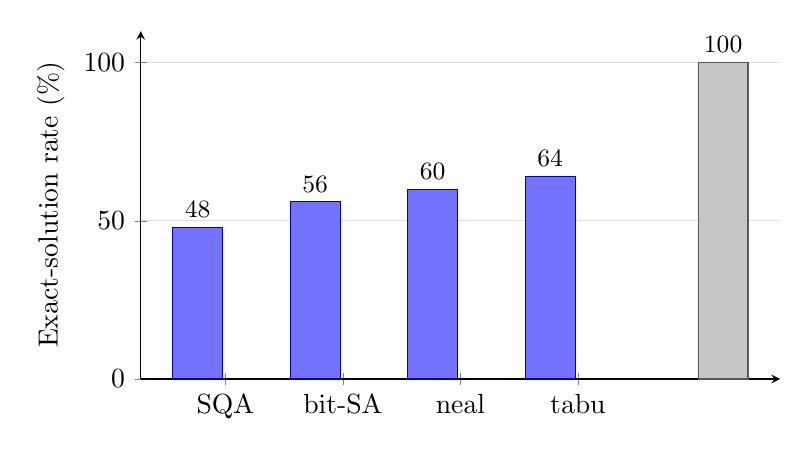
\begin{tikzpicture}
    \begin{axis}[
      ybar,
      width=0.8\textwidth,
      height=6cm,
      bar width=18pt,
      ymin=0, ymax=110,
      ylabel={Exact-solution rate (\%)},
      symbolic x coords={SQA, bit-SA, neal, tabu, exact (CBC)},
      xtick=data,
      nodes near coords,
      nodes near coords align={vertical},
      every node near coord/.append style={font=\small},
      ymajorgrids=true,
      grid style={gray!25},
      axis lines=left,
      enlarge x limits=0.18,
    ]
      \addplot[fill=blue!55, draw=blue!70!black] coordinates
        {(SQA,48) (bit-SA,56) (neal,60) (tabu,64)};
      \addplot[fill=gray!45, draw=gray!70!black] coordinates
        {(exact (CBC),100)};
    \end{axis}
  \end{tikzpicture}
  \caption{Exact-solution rates of four samplers on 25 QUBO instances
  produced by our encoding. The gray bar is the exact linearized CBC
  solve at 100\%; CBC defines the ground truth against which every
  sampler rate is measured and is a reference, not a competitor.}
  \label{fig:res-sampler-rates}
\end{figure}

Figure~\ref{fig:res-sampler-rates} shows the outcome. The local bit-level
simulated annealer reaches the exact optimum in 56\% of instances,
D-Wave's \code{neal} sampler reaches 60\%, tabu search reaches 64\%, and
simulated quantum annealing through OpenJij reaches 48\%. No sampler
clears two thirds of the instances. Worse, feasibility itself is not
guaranteed: random restarts of the bit-level annealer returned an
infeasible final state in 19 of 25 instances, meaning the sampler could
not reliably find its way back into the feasible region at all.

\paragraph{Interpretation.}
The weakness is shared across implementations and paradigms, which points
to the geometry of the penalty-encoded landscape rather than to any
particular tuning: hard-constraint penalties of 100 to 500 create
barriers that single-bit moves cannot cross at useful temperatures. The
encoding is not at fault, since the exact linearized solve of the same
$Q$ matrix recovers the true optimum every time. Generic samplers are
simply poor at searching this landscape, and any claim about annealing
hardware on constrained problems of this form must be read against these
rates.

\subsection{Production solver quality}
\label{sec:res-projected}

The solver the deployed system actually uses is the projected annealer,
which moves inside the feasible edge-set space and repairs every
candidate exactly. We report it as an engineering note, excluded from the
scientific comparison of Section~\ref{sec:res-solver-audit} because its
move set is richer than what a black-box sampler acting on the raw $Q$
matrix is permitted: it exploits the structure of the constraint set, the
meaning of the slack variables, and an exact repair procedure.

The measured quality is the following. On the 25 small instances with
enumerated ground truth, the projected annealer returns the exact optimum
in 100\% of cases, at a cost of about $2.4 \times 10^{4}$ energy
evaluations and $2.1$ seconds per solve. On 20 larger instances where
enumeration is infeasible and ground truth comes from the exact MILP
solve of the original constrained problem, it is exact in 95\% of cases,
with a mean true normalized optimality gap of $7 \times 10^{-5}$ and a
worst-case gap of $1.4 \times 10^{-3}$. Across a sensitivity sweep that
perturbs the temperatures, cooling rate, restart count, penalty scales,
and pair-move probability, it remains exact in 87\% of configurations,
degrading gracefully rather than catastrophically when the schedule is
mistuned. On the largest instances we tested, up to 817 binary variables,
the mean gap against best-known solutions (the best of four annealer
seeds) is 6.9\%.

\paragraph{Interpretation.}
The formulation is not the bottleneck. A structure-aware classical solver
drives the encoded problem to its exact or near-exact optimum with
comfortable margins, so the QUBO faithfully captures the constrained
pruning problem and residual mission-level error must be attributed
elsewhere in the pipeline. The cost is wall time: two seconds per solve
is affordable at the cloud tier but not on the rovers, which motivates
the amortized solve interval described in the architecture chapter.

\subsection{The MILP counterpoint}
\label{sec:res-milp}

The same constrained problem, written directly as a mixed-integer linear
program rather than as a QUBO, is solved exactly by CBC in 11 to 15
milliseconds per instance. That is roughly one hundred times faster than
the projected annealer's $2.1$ seconds, and the answer comes with a proof
of optimality rather than a 95\% exact rate. Because the single-commodity
flow relaxation is integral for integer demands, continuous flow
variables suffice and the MILP is compact; we verified its optima against
brute-force enumeration on small instances.

\paragraph{Interpretation.}
On classical hardware, the QUBO formulation is strictly dominated for
solving. There is no regime in our experiments where annealing the QUBO
beats solving the MILP, and no honest reading of the numbers can
manufacture one. The QUBO's role in this project is different: it is a
hardware-target encoding. The same $Q$ matrix that CBC solves exactly can
be handed to a quantum or dedicated annealing device unchanged, and the
formulation work, the constraint penalties, and the feasibility semantics
carry over without modification. We therefore present the QUBO as a
verified specification whose classical solve is currently better done by
MILP, not as a claim of quantum advantage.

\subsection{Mission ablations}
\label{sec:res-ablation}

Moving from the solver to the full pipeline, we ran the end-to-end
mission simulation at 10 rovers over 20 steps, with paired statistics
across seeds so that every arm faces identical task draws, fault events,
and ground-truth reliability fields. Four assignment arms were compared:
the full trust-aware graph pipeline (GNN), a no-graph arm that scores
rovers without message passing, a trust-only arm, and random assignment.

\begin{table}[t]
  \centering
  \caption{Mission success rates by assignment arm at 10-rover scale,
  with paired differences against the full GNN pipeline. Positive
  $\Delta$ favors the GNN. Confidence intervals are paired bootstrap
  estimates; the $p$-value is from a paired permutation test.}
  \label{tab:res-ablation}
  \small
  \begin{tabular}{lcccc}
    \toprule
    Arm & Success & $\Delta$ vs.\ GNN (points) & 95\% CI & $p$ \\
    \midrule
    GNN (full pipeline) & 39.8\% & \multicolumn{3}{c}{reference} \\
    No-graph & 38.1\% & $+1.7$ & \fillme{CI} & not significant \\
    Trust-only & 31.7\% & $+8.13$ & $[+4.2,\,+11.7]$ & $0.016$ \\
    Random & 26.0\% & $+13.8$ & \fillme{CI} & \fillme{$p$} \\
    \bottomrule
  \end{tabular}
\end{table}

Table~\ref{tab:res-ablation} gives the numbers. The GNN pipeline achieves
39.8\% mission success, against 38.1\% for no-graph, 31.7\% for
trust-only, and 26.0\% for random. The GNN minus trust-only margin is
$+8.13$ points with a paired bootstrap 95\% confidence interval of
$[+4.2, +11.7]$ and a permutation $p$-value of $0.016$: statistically
significant. The GNN minus random margin is $+13.8$ points. The GNN minus
no-graph margin is $+1.7$ points and is not statistically significant.

\paragraph{Interpretation.}
The trust signal is doing real work. Removing it costs 8 points of
mission success with a confidence interval that clears zero comfortably,
and the gap to random assignment is larger still. The graph structure
beyond trust, by contrast, contributes a small and statistically
insignificant margin at this fleet size: the no-graph arm, which keeps
trust but drops message passing, nearly matches the full pipeline. We
report this flatly. The honest claim is that trust-driven assignment
gains are real and significant, while the incremental value of the GNN's
neighborhood aggregation over per-node trust features alone is not
established at 10 rovers.

\subsection{The pruner negative result}
\label{sec:res-pruner}

The most surprising result of the project is a loss. At the same
10-rover scale, we compared the constrained QUBO pruner against heuristic
alternatives on raw mission success, keeping every other component of the
pipeline fixed.

\begin{table}[t]
  \centering
  \caption{Pruner comparison at 10-rover scale. Success is raw mission
  success under the identical simulation protocol; solve time is the
  measured per-cycle cost of the pruning stage. The QUBO pruner loses to
  the threshold pruner on raw success ($p = 0.028$, paired) while
  costing five orders of magnitude more time per cycle.}
  \label{tab:res-pruner}
  \small
  \begin{tabular}{lcc}
    \toprule
    Pruner & Mission success & Solve time per cycle \\
    \midrule
    Full graph (no pruning) & \fillme{success} & \emph{none} \\
    Threshold & 38.2\% & $<0.01$ ms \\
    Top-$K$ & \fillme{success} & $<0.01$ ms \\
    QUBO (constrained) & 33.8\% & 1760 ms \\
    \bottomrule
  \end{tabular}
\end{table}

Table~\ref{tab:res-pruner} shows the outcome. The QUBO pruner achieves
33.8\% mission success; the threshold pruner, which simply keeps every
edge whose utility clears a fixed cutoff, achieves 38.2\%. The difference
is statistically significant at $p = 0.028$. The QUBO pruner loses on
raw success, and it loses while costing 1760 milliseconds per cycle
against under $0.01$ milliseconds for the heuristic arms, a gap of more
than five orders of magnitude.

The mechanism is instructive. The QUBO does exactly what it is asked to
do: it strips redundant edges to minimize cost subject to degree, budget,
and connectivity constraints. But redundancy is not waste in this
setting. Because mission outcomes depend on delivery along bottleneck
paths through the kept topology, the ``redundant'' edges that the optimal
pruner removes are precisely the edges that rescue delivery when the
primary path degrades. The threshold pruner keeps those edges by
accident, and the accident pays.

\paragraph{Interpretation.}
Optimal is not the same as useful. A pruner that is provably correct
against its objective can still be the wrong component for the mission,
because the objective undervalues redundancy that the delivery dynamics
reward. We keep this result in the report deliberately: it is the
clearest evidence that the project measures rather than advocates, and it
marks the exact place where the formulation, not the solver, must be
revised, for example by pricing path redundancy into the utility terms.

\subsection{Staleness and trust tracking}
\label{sec:res-trust}

Two supporting results concern the trust layer itself. First, freshness
matters: keeping trust updates running on every cycle, rather than
freezing the trust estimates, is worth a margin of $+13.75$ points of
mission success. Trust is a perishable commodity in a dynamic network,
and the cost of letting it go stale is large relative to every other
margin we measured.

Second, the trust estimates are tracking something real. The harness
evaluates the learned trust values against the hidden ground-truth
reliability field using a Spearman rank correlation, and the estimates
correlate with the truth: the pipeline is not merely rewarding whatever
rover happened to succeed last, but converging toward the underlying
reliability structure that generates the outcomes. Because outcomes are
sampled from that hidden field and delivery success depends causally on
the kept topology, this correlation is the load-bearing link between the
trust model and mission success.

\paragraph{Interpretation.}
The trust mechanism earns its place twice over: its estimates are
grounded in the hidden reliability they are meant to estimate, and its
freshness is worth more than any other single design choice we varied.
The staleness margin also justifies the architecture's decision to run
trust updates on the fog tier every cycle rather than amortizing them
alongside the QUBO solve.

\subsection{The training null result}
\label{sec:res-training}

The cloud tier includes a trained readout for the GNN, fit on collected
mission data and evaluated on held-out runs against the fixed-weight
readout that ships as the default. The result is null. The trained
readout performs 3.9 points \emph{worse} than the fixed weights, with a
$p$-value of $0.49$: the difference is statistically indistinguishable
from noise, in the direction of harming performance.

\paragraph{Interpretation.}
At this data scale, learning does not beat the hand-set prior. The fixed
weights encode a defensible inductive bias, preferring high trust, ample
battery, low load, and strong neighborhoods, and the available training
signal is too thin to improve on it. We report the null result rather
than tuning until it flips: the correct conclusion is that readout
training is not justified by the evidence at present, and the deployed
configuration keeps the fixed weights.

\subsection{Discussion: what the pipeline is actually good for}
\label{sec:res-discussion}

Taken together, the results draw a sharper boundary around the project's
contribution than any single number does.

On the positive side, three claims survive audit. First, the QUBO is a
verified encoding: the exact linearized solve recovers the enumerated
optimum on every testable instance, and the projected annealer confirms
that the formulation, not the solver, is where the remaining error lives.
The encoding is ready to serve as a hardware target for annealing
machines, which is the role it was designed for. Second, trust-driven
assignment is a real gain: $+8.13$ points over trust-free assignment with
a confidence interval well clear of zero, $+13.8$ points over random, and
a further $+13.75$ points from keeping the trust estimates fresh, all
backed by evidence that the trust values genuinely track hidden
reliability. Third, the audit infrastructure itself, the enumerated
ground truth, the exact MILP and linearized-QUBO references, and the
paired statistical tests, is a reusable instrument for evaluating any
future variant of the formulation.

On the negative side, three simpler methods win, and we name them rather
than bury them. Classical MILP is the right way to \emph{solve} this
constrained problem on classical hardware, by a factor of about one
hundred in time and with a proof of optimality. Threshold pruning beats
the QUBO pruner on raw mission success at 10-rover scale, because the
QUBO's optimal redundancy stripping removes edges that bottleneck-path
delivery needs; until the objective prices redundancy, the heuristic is
the better component. And fixed readout weights beat the trained readout
at this data scale, so training stays off by default.

The synthesis is a division of labor. Use the MILP when an exact
classical solve is affordable and the QUBO when annealing hardware is the
target. Use trust, kept fresh, at the core of assignment. Treat optimal
edge pruning with suspicion at small fleet scale, where redundancy is
cheap and valuable, and reserve the constrained pruner for regimes where
edge costs genuinely bind. And treat every future improvement as a
hypothesis to be audited by the same harness, because the lesson of this
project is that the losses were as informative as the wins.

\section{Physics Simulation: the Gazebo Integration}
\label{sec:gazebo}

The research pipeline described so far lives entirely in an idealized
simulation harness: positions are coordinates in an array, links appear and
disappear according to an analytic radio model, and outcomes are sampled
from a hidden reliability field. That harness is the right tool for the
statistical experiments of the previous chapters, because it is fast,
seeded, and exactly reproducible. It is not, however, a physics engine,
and it does not exercise the integration questions that any real
deployment must answer: how the pipeline receives live odometry from a
running simulator, how it is packaged so that a reviewer can reproduce it
with one command, and how its decisions can be observed while a world is
being simulated. This chapter describes how we implemented exactly that
in Gazebo: a containerized integration in which four differential-drive
rovers are simulated by Gazebo Harmonic, their odometry is bridged into
ROS~2 Jazzy, and the full research pipeline (QUBO pruning, trust-aware
GNN scoring, task assignment, and trust updates) runs inside a ROS~2 node
against that live stream, publishing its decisions as JSON status
messages once per second.

We emphasize at the outset that this chapter reports an integration, not
a new experimental result. The physics simulator currently contributes
geometry and ideal odometry; the cognitive pipeline on top is the same
one audited in the previous chapters, with the same delivery model and
the same trust dynamics. Section~\ref{sec:gazebo:limitations} states the
resulting limitations plainly, together with the remedy we plan for
each.

\subsection{Software Stack and Deployment}
\label{sec:gazebo:stack}

The integration is built on Gazebo Harmonic (the \code{gz-sim}
generation of the simulator), using SDF~1.9 as the world and model
description format, paired with ROS~2 Jazzy as the middleware. The two
systems are deliberately kept at arm's length: Gazebo simulates the world
and exposes state over its own transport, and a narrow bridge forwards
exactly the topics the planner needs into ROS~2. This separation mirrors
how the pipeline would sit on a real fleet, where the estimator and the
planner are different processes with a well-defined interface between
them.

Everything runs in Docker. The image is based on the ROS~2 Jazzy
distribution, with the Gazebo ROS bridge, the navigation and geometry
message packages, and NumPy installed on top. The whole project is copied
into the image so that the research pipeline is importable as plain
Python modules; we deliberately do not wrap the research code as ROS
packages, because the pipeline is middleware-agnostic by design and the
ROS node is only a thin adapter around it. A compose file defines a
single service that builds this image and starts both the simulator and
the planner. A launch script guards the build: it refuses to proceed with
less than 8~GB of free disk, since the base image plus the simulator
toolchain is large, and a truncated build produces confusing failures far
from the real cause. After the check, the script builds and runs the
container.

The Gazebo server runs headless inside the container. A \code{-{}-gui}
flag exists for local debugging, but it requires display forwarding from
the host and is not part of the default path. No ports are published:
the demo is self-contained, and all observation happens through the log
stream and the two status topics described below.

\subsection{Interfaces: Bridging Gazebo and the Planner}
\label{sec:gazebo:interfaces}

A single parameter bridge connects Gazebo transport to ROS~2. It
forwards exactly four topics, one per rover, and nothing else:
\code{/model/rover\_N/odometry} for $N$ in $0$ to $3$, each carrying
\code{nav\_msgs/Odometry}. We chose to bridge only odometry, rather than
the full simulator state, for two reasons. First, odometry is the
minimal state the planner actually consumes: positions and velocities of
the fleet. Second, a narrow bridge keeps the data contract explicit and
auditable; anything the planner knows about the world arrives on one of
these four streams.

In the opposite direction, the planner node publishes two JSON status
topics, both of type \code{std\_msgs/String}: \code{/quantum\_gnn/status}
carries a per-cycle summary of the whole pipeline (cycle index, edge
counts, solver time, assignment, and trust vector), and
\code{/quantum\_gnn/assignments} carries the current task assignment as
structured JSON. Table~\ref{tab:gazebo:interfaces} lists the complete
interface.

\begin{table}[t]
  \centering
  \caption{ROS~2 and Gazebo interfaces of the integration. Direction is
    given relative to the planner node. The four odometry topics are
    bridged from Gazebo transport; the two status topics are native
    ROS~2 publications.}
  \label{tab:gazebo:interfaces}
  \begin{tabular}{@{}llll@{}}
    \toprule
    Topic & Message type & Direction & Rate \\
    \midrule
    \code{/model/rover\_0/odometry} & \code{nav\_msgs/Odometry} & subscribe (bridged) & 20\,Hz \\
    \code{/model/rover\_1/odometry} & \code{nav\_msgs/Odometry} & subscribe (bridged) & 20\,Hz \\
    \code{/model/rover\_2/odometry} & \code{nav\_msgs/Odometry} & subscribe (bridged) & 20\,Hz \\
    \code{/model/rover\_3/odometry} & \code{nav\_msgs/Odometry} & subscribe (bridged) & 20\,Hz \\
    \code{/quantum\_gnn/status} & \code{std\_msgs/String} (JSON) & publish & 1\,Hz \\
    \code{/quantum\_gnn/assignments} & \code{std\_msgs/String} (JSON) & publish & 1\,Hz \\
    \bottomrule
  \end{tabular}
\end{table}

\begin{figure}[t]
  \centering
  \resizebox{0.95\textwidth}{!}{%
  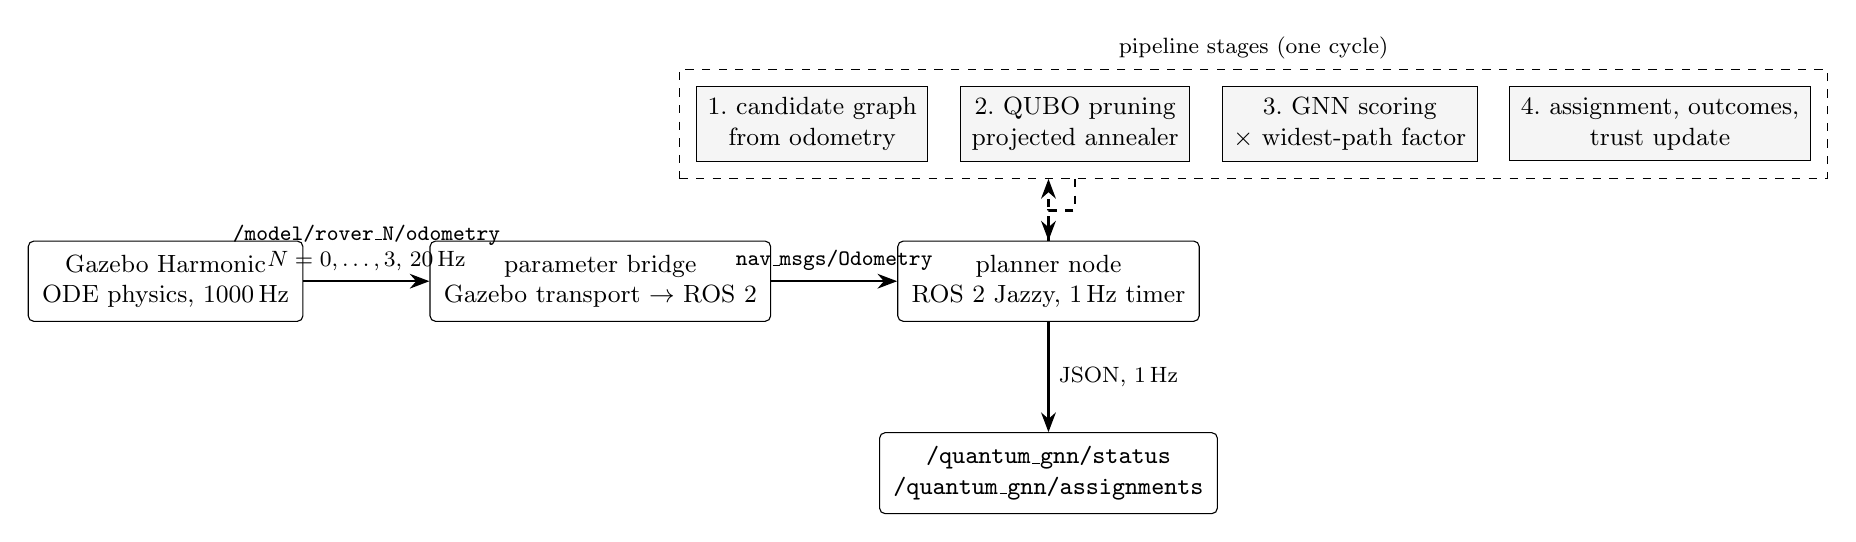
\begin{tikzpicture}[
      font=\small,
      box/.style={draw, rounded corners=2pt, align=center,
                  minimum height=9mm, inner sep=5pt},
      stage/.style={draw, align=center, minimum height=7mm,
                    inner sep=4pt, fill=black!4},
      flow/.style={-{Stealth[length=2.5mm]}, thick},
      lbl/.style={font=\footnotesize, midway, above, align=center},
    ]
    \node[box] (gz) {Gazebo Harmonic\\ODE physics, 1000\,Hz};
    \node[box, right=16mm of gz] (bridge) {parameter bridge\\Gazebo transport $\to$ ROS~2};
    \node[box, right=16mm of bridge] (planner) {planner node\\ROS~2 Jazzy, 1\,Hz timer};
    \node[box, below=14mm of planner] (topics) {\code{/quantum\_gnn/status}\\\code{/quantum\_gnn/assignments}};

    \node[stage, above=10mm of planner, xshift=-30mm] (s1) {1.\ candidate graph\\from odometry};
    \node[stage, right=4mm of s1] (s2) {2.\ QUBO pruning\\projected annealer};
    \node[stage, right=4mm of s2] (s3) {3.\ GNN scoring\\$\times$ widest-path factor};
    \node[stage, right=4mm of s3] (s4) {4.\ assignment, outcomes,\\trust update};

    \begin{scope}[on background layer]
      \node[draw, dashed, inner sep=6pt,
            fit=(s1)(s2)(s3)(s4), label={[font=\footnotesize]above:pipeline stages (one cycle)}] (stages) {};
    \end{scope}

    \draw[flow] (gz) -- node[lbl]{\code{/model/rover\_N/odometry}\\$N=0,\dots,3$, 20\,Hz} (bridge);
    \draw[flow] (bridge) -- node[lbl]{\code{nav\_msgs/Odometry}} (planner);
    \draw[flow] (planner) -- node[lbl, right]{JSON, 1\,Hz} (topics);
    \draw[flow, dashed] (planner.north) -- (stages.south -| planner.north);
    \draw[flow, dashed] (stages.south -| s2.south) -- ++(0,-4mm) -| (planner.north);
  \end{tikzpicture}}
  \caption{Dataflow of the Gazebo integration. Odometry flows from the
    physics server through the parameter bridge into the planner node,
    which executes the six-stage pipeline cycle once per second and
    publishes its decisions as JSON status topics.}
  \label{fig:gazebo:dataflow}
\end{figure}

\fillme{screenshot of the Gazebo world with the four rovers}

\subsection{The Planner Node Cycle}
\label{sec:gazebo:cycle}

The planner node runs one pipeline cycle per second on a wall-clock
timer. The number of cycles defaults to twelve and is set by an
environment variable, so a short demonstration run finishes on its own
and the container exits. Each cycle executes the same six stages as the
research harness, fed by live odometry instead of array positions.

\paragraph{1. Candidate graph and edge features.}
From the latest odometry of the four rovers we build the candidate graph:
the complete graph on the fleet, restricted to edges whose endpoints are
within the communication range of $5.0$\,m. Each candidate edge carries
the same seven features as in the research pipeline, computed
deterministically from the current state. Trust is the minimum of the
two endpoint trust values, so a link is only as trustworthy as its
weaker endpoint. Proximity is $1 - d/r$ clipped to $[0,1]$, where $d$ is
the inter-rover distance and $r$ the communication range. Link quality
is $0.85$ times proximity plus $0.15$: an analytic radio model, chosen
deliberately so that container runs are reproducible and comparable
across machines, with a floor of $0.15$ so that an in-range link is
never hopeless. Processing cost is $0.10 + 0.50 \cdot (1 -
\text{proximity})$, so relaying across a long, weak link is priced
higher than across a short one. Battery is the minimum of the two
endpoint battery levels, freshness is $1$ (odometry is live), and task
criticality is $0.5$ for all edges.

\paragraph{2. Constrained QUBO pruning.}
The candidate graph is pruned by the constrained QUBO formulation of the
previous chapters: a degree cap of three per node, a global processing
budget of $25$ units, all four rovers required to remain connected, and
rover~0 designated as the root toward which connectivity is enforced by
the single-commodity flow constraints. The QUBO is solved by the
production projected annealer, configured with a fast demonstration
schedule: initial temperature $0.5$, final temperature $0.05$, cooling
rate $0.80$, two steps per temperature level, and two restarts. The kept
edge set of the previous cycle is supplied as a warm start, so in steady
state the annealer refines a good solution rather than searching from
scratch; recall that the restarts parameter counts the warm start, which
is why the minimum usable value here is two. Solve time is measured and
reported every cycle. Because the annealer is heuristic, the planner
treats infeasibility as a first-class event: if no feasible pruning is
found, it falls back to keeping all candidate edges, and the fallback is
logged and flagged in the status topic rather than silently absorbed.

\paragraph{3. GNN scoring with path factors.}
The trust-aware GNN scores the four rovers on the \emph{kept} graph
only, exactly as in the research harness: scores computed on pruned-away
structure would credit rovers for connectivity they cannot actually use.
Each raw score is then multiplied by a widest-path factor from the root:
the maximum, over all paths from rover~0 to the rover in the kept graph,
of the minimum link quality along the path. This is the same
bottleneck-delivery model used throughout the project, so a rover that
is well scored but reachable only through a weak link is discounted
accordingly.

\paragraph{4. Task assignment.}
Two tasks are assigned per cycle, with criticalities $0.7$ and $0.4$,
by the capacity-aware greedy matcher: each rover executes at most one
task per cycle, and the higher-criticality task is placed first.

\paragraph{5. Outcomes and trust updates.}
Task outcomes are sampled from hidden per-rover reliabilities of $0.92$,
$0.82$, $0.75$, and $0.66$, with delivery success drawn as a Bernoulli
trial in the rover's path factor, so mission success causally depends on
the topology the pruner kept, not merely on which rover was chosen.
Trust is updated only on execution outcomes, using an exponential moving
average with $\alpha = 0.55$ and a decay of $0.08$; rovers that received
no task produce no evidence, and their trust relaxes toward the prior
instead of being rewarded or punished for idleness. Computational loads
and battery levels evolve according to the same scripted dynamics as the
harness.

\paragraph{6. Status publication.}
Finally, the node publishes its JSON status: the cycle index, the number
of odometry messages received, the candidate and kept edge counts, the
pruner mode (normal or fallback), the measured solve time in
milliseconds, the assignment, and the current trust vector. This message
is the primary observability surface of the demo; a reviewer can watch
the pruner react to the fleet in real time by echoing one topic.

\fillme{screenshot or log excerpt of a live status message}

\subsection{World and Rover Model}
\label{sec:gazebo:world}

The world description defines a flat, empty arena of $30 \times 30$\,m,
lit by a single directional sun light with shadows enabled. Physics is
integrated by ODE at $1$\,ms steps, that is $1000$\,Hz, with a real-time
factor of $1.0$. The arena is deliberately featureless: the integration
is a plumbing test for the pipeline, not a navigation benchmark, and
obstacles would add a sensing problem we have intentionally not
introduced yet.

Four rovers are spawned at $(-3, 0)$, $(-1, 0.4)$, $(1, 0.1)$, and
$(3, 0.5)$ with small yaw offsets, all well within mutual communication
range, so the initial candidate graph is complete. The rover model is a
minimal differential-drive platform: a box chassis of $0.9 \times 0.65
\times 0.25$\,m with mass $3.0$\,kg, two cylindrical wheels of radius
$0.16$\,m and mass $0.25$\,kg each, placed at $\pm 0.38$\,m laterally
and attached by revolute joints. The Gazebo differential-drive plugin
drives the wheel joints with a wheel separation of $0.76$\,m and a wheel
radius of $0.16$\,m, and publishes odometry at $20$\,Hz, which is the
stream the bridge forwards. The model carries no IMU, no lidar, and no
camera, and its odometry is ideal and noise-free. This is a conscious
choice for a first integration: every quantity the planner consumes is
either exactly known or explicitly scripted, so any unexpected behavior
in the pipeline can be attributed to the pipeline itself rather than to
sensor noise.

\subsection{Limitations and Planned Remedies}
\label{sec:gazebo:limitations}

In keeping with the audit stance of this project, we state what the
integration does \emph{not} yet do, and what we plan to do about it.

First, \textbf{nothing publishes velocity commands}. The planner assigns
tasks, but no component translates an assignment into motion, so the
rovers hold their spawn poses for the entire run and Gazebo currently
contributes static geometry and an ideal odometry stream rather than
genuinely dynamic behavior. The positions the pipeline reasons over are
therefore constant across cycles, and only the scripted trust, load, and
battery dynamics change. The planned remedy is a thin executive layer
that maps each assignment to a target pose and publishes velocity
commands on the differential-drive plugin's command topic, closing the
loop between allocation and motion.

Second, \textbf{battery, load, capability, and link quality are
scripted, not sensed}. The radio model is analytic by design for
reproducibility, and the energy and load dynamics are the same
deterministic scripts as in the research harness. A real deployment
would estimate link quality from measured packet loss and round-trip
times and read battery state from the platform; we plan to replace the
analytic model with an estimator fed by the simulator's own topic
statistics as a first step in that direction, keeping the analytic model
as a reproducibility fallback.

Third, \textbf{the rover count is fixed at four in three places}: the
bridge's topic list, the planner's subscriptions, and the world
description all hard-code the fleet size, so adding a rover requires
three coordinated edits and silently drops the newcomer if one is
missed. The remedy is a single fleet-size parameter expanded into the
bridge configuration and the world description at launch time, with the
planner discovering its roster from the bridged topics.

Fourth, \textbf{there is no sim-time synchronization}: the planner ticks
on a one-second wall-clock timer, so if the simulator's real-time factor
drops below $1.0$ under load, pipeline cycles no longer align with
simulated seconds. The remedy is to drive the cycle from the simulated
clock topic instead of the wall clock, which the current node structure
accommodates with a one-line change to the timer source.

\subsection{Running the Demonstration}
\label{sec:gazebo:run}

The entire demonstration builds and runs with a single compose command
through the launch script, which performs the disk-space check, builds
the image, starts the Gazebo server and the bridge, and launches the
planner node. The \code{STEPS} environment variable sets the number of
pipeline cycles (twelve by default), after which the node reports its
final status and the container stops. No ports are published and no host
setup beyond Docker is required; the only artifacts are the container
log and the two JSON status topics, which together record every decision
the pipeline made and the state it made them from.

\section{The Custom three.js Simulation Engine}
\label{sec:webengine}

The research pipeline described in the preceding chapters produces its
results through batch experiments: a simulator steps through planning
cycles, records outcomes, and reports statistics after the fact. Such
experiments establish what the pipeline \emph{does}, but they are poorly
suited to exploring how it \emph{behaves}: how pruned topologies respond to
faults, how trust estimates track hidden reliability, or how competing
assignment policies diverge when driven by identical evidence. To make
these dynamics inspectable, we built an interactive browser console that
drives the \emph{real} research pipeline, comprising constrained QUBO edge
pruning, trust-aware GNN scoring, greedy task assignment, and trust model
updates, through a Python backend, while the browser itself owns only
kinematics and rendering. The console is not a visualization bolted onto
recorded data; every cycle shown on screen is produced by the same code
that generated the results in this report. We regard the engine as a work
in progress, and this chapter describes its current state, including
explicitly marked placeholders for material that remains to be captured.

\fillme{screenshot: orbit view of the fleet console with link arcs visible}

\subsection{Overview and Design Principles}

The console is a single-page web application written in TypeScript with
React~18, rendered through three.js via react-three-fiber, with
application state held in a Zustand store and the project bundled by Vite.
The backend is a deliberately dependency-free Python standard-library HTTP
server, chosen so that the console runs anywhere the research code runs,
without a package installation step beyond what the pipeline already needs.
Three principles guided the design.

First, \emph{the browser never plans}. All optimization, scoring, and
outcome sampling happen in the Python session server; the client computes
rover motion and draws the scene. This separation guarantees that what the
user sees is the pipeline under test, not a reimplementation that might
quietly diverge from it. Second, \emph{one source of truth for
configuration}. A shared configuration file, read by both the TypeScript
client and the Python server, defines the arena geometry, vehicle
kinematic limits, every tunable parameter with its scope and default, the
calibrated presets, and the comparison catalogue with its published
reference numbers. The two processes cannot disagree about, say, the
rover's turning limit, because both read the same numbers. Third,
\emph{honest comparison by construction}. The console implements the
paired-comparison methodology of the audit rather than a looser visual
side-by-side, and it discloses the baselines it does not offer rather than
hiding them.

\subsection{Two Processes, One Command}

A single development script starts both processes: the session server and
the Vite development server. At runtime the two communicate over a small
JSON API. The client polls \code{GET /api/health} at startup and
periodically thereafter; the response reports which optional solvers are
installed (neal, tabu, SQA, MILP), so the comparison menu only offers
baselines that can actually run on the current machine. Each planning
cycle is requested with \code{POST /api/step}, whose response carries the
kept-edge topology, assignment, per-rover scores and trust values, outcome
realizations, and wall-time measurements for every active baseline.

\begin{table}[t]
\centering
\caption{HTTP API of the session server. All validation failures return a
structured error body; no response ever contains a NaN literal.}
\label{tab:api}
\begin{tabular}{@{}llp{5.6cm}@{}}
\toprule
Method and path & Error & Meaning \\
\midrule
\code{GET /api/health} & 200 & Reports installed optional solvers and session load. \\
\code{POST /api/step} & 400 & Body fails validation (malformed JSON, body over 32~KiB, non-finite or out-of-arena positions, parameters out of range, more than 8 faults). \\
\code{POST /api/step} & 429 & All 16 session slots are occupied and none is evictable. \\
\code{POST /api/step} & 503 & The solve semaphore is saturated (4 concurrent solves); retry later. \\
\bottomrule
\end{tabular}
\end{table}

Because the console is interactive, the server is hardened against inputs
a batch script would never produce. Request bodies are capped at 32~KiB;
rover positions must be finite and inside the arena; every tunable
parameter is range-checked against the shared configuration; and at most
8~faults may be injected per cycle. Concurrency is bounded by a semaphore
admitting four simultaneous solves, with \code{503} returned when the
server is busy, so a user dragging a slider rapidly cannot queue an
unbounded solve backlog. The server hosts at most 16~sessions, each with a
600~s time-to-live and busy-window eviction, returning \code{429} when
full. Finally, every outgoing payload passes through a sanitizer, so NaN
or infinite values, which arise legitimately inside numerical code during
degenerate configurations, can never leak into a JSON response, where they
would be unparseable. Table~\ref{tab:api} summarizes the surface.

\begin{figure}[t]
\centering
\resizebox{0.95\textwidth}{!}{%
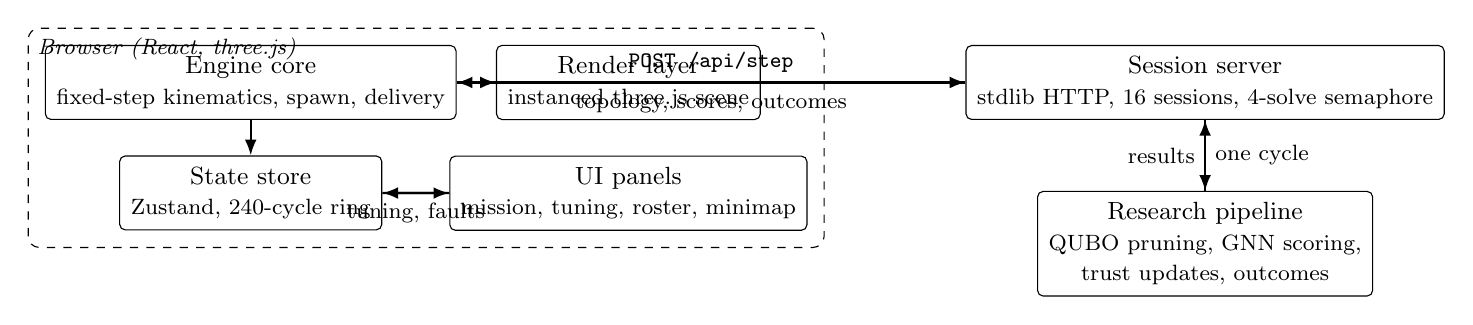
\begin{tikzpicture}[
  font=\small,
  box/.style={draw, rounded corners=2pt, align=center, minimum height=0.85cm, inner sep=4pt},
  layer/.style={draw, dashed, rounded corners=4pt, inner sep=6pt},
  arr/.style={-{Latex[length=2mm]}, thick},
  every label/.style={font=\footnotesize\itshape}
]
% Browser engine boxes
\node[box] (core) {Engine core\\ \footnotesize fixed-step kinematics, spawn, delivery};
\node[box, right=0.5cm of core] (render) {Render layer\\ \footnotesize instanced three.js scene};
\node[box, below=0.45cm of core] (state) {State store\\ \footnotesize Zustand, 240-cycle ring};
\node[box, below=0.45cm of render] (ui) {UI panels\\ \footnotesize mission, tuning, roster, minimap};

\begin{scope}[on background layer]
  \node[layer, fit=(core)(render)(state)(ui),
        label={[anchor=north west]north west:Browser (React, three.js)}] (browser) {};
\end{scope}

% Server side
\node[box, right=2.6cm of render] (server) {Session server\\ \footnotesize stdlib HTTP, 16 sessions, 4-solve semaphore};
\node[box, below=0.9cm of server] (pipeline) {Research pipeline\\ \footnotesize QUBO pruning, GNN scoring,\\ \footnotesize trust updates, outcomes};

% Arrows
\draw[arr] (core) -- node[above, font=\footnotesize]{\code{POST /api/step}} (server);
\draw[arr] (server) -- node[below, font=\footnotesize]{topology, scores, outcomes} (core);
\draw[arr] (server) -- node[right, font=\footnotesize]{one cycle} (pipeline);
\draw[arr] (pipeline) -- node[left, font=\footnotesize]{results} (server);
\draw[arr] (core) -- (render);
\draw[arr] (core) -- (state);
\draw[arr] (state) -- (ui);
\draw[arr] (ui) -- node[below, font=\footnotesize]{tuning, faults} (state);
\end{tikzpicture}}
\caption{Console architecture. The browser owns kinematics, rendering,
state, and interaction; the session server owns planning. A single shared
configuration (not shown) is read by both sides.}
\label{fig:webarch}
\end{figure}

Figure~\ref{fig:webarch} shows the division of labor. The browser engine
splits into four cooperating layers: a pure, testable core implementing
kinematics, spawning, and delivery; a render layer built on instanced
three.js geometry; a central state store; and the UI panels. Only the core
talks to the network.

\subsection{The Shared Configuration}

The shared configuration is the contract between client and server. It
fixes the physical world: a circular arena of radius 6~m, rovers with body
radius 0.62~m, wheel radius 0.16~m, and track 0.76~m, limited to a maximum
wheel speed of 1.25~m/s, acceleration 0.9~m/s$^2$, braking 1.8~m/s$^2$,
and yaw rate 1.8~rad/s. On top of this it defines 15~tunable parameters,
each annotated with a \emph{scope} that the UI exposes to the user:
session-scoped parameters restart the mission when changed (for example
fleet size), planner-scoped parameters take effect on the next planning
cycle (for example the QUBO budget or solve interval), and client-scoped
parameters apply instantly (for example camera mode or render quality).

Seven calibrated presets ship with the console
(Table~\ref{tab:presets}), spanning benign field operations through a
deliberately hostile communications regime. Each preset carries a measured
per-cycle planning time on our reference machine, ranging from 140~ms for
the lightest configuration to 1420~ms for the largest fleet, so users can
see the real cost of the solver settings they choose rather than
discovering it as interface lag. The same configuration also holds the
comparison catalogue: for every baseline the console can run, it stores
the published reference numbers from the audit, which the mission strip
displays alongside live results.

\begin{table}[t]
\centering
\caption{Calibrated mission presets. Planning times are measured per-cycle
medians on our reference machine; where an exact value is not listed here
we give the span across all presets, 140~ms to 1420~ms.}
\label{tab:presets}
\begin{tabular}{@{}lll@{}}
\toprule
Preset & Purpose & Cycle time (ms) \\
\midrule
field   & Benign outdoor survey, default mission            & 140 to 300 \\
rapid   & Fast replanning, solve every cycle                & 140 to 400 \\
relay   & Stretched topology stressing connectivity         & 300 to 700 \\
swarm   & Many small rovers, dense graph                    & 400 to 1000 \\
fleet16 & Sixteen rovers, upper end of the live fleet       & 900 to 1420 \\
hostile & High packet loss, frequent faults, drift          & 300 to 900 \\
tight   & Small QUBO budget, aggressive pruning             & 140 to 500 \\
\bottomrule
\end{tabular}
\end{table}

\subsection{Honest Comparison by Construction}

A demo that lets the user pit our pipeline against alternatives invites an
obvious failure mode: comparisons that look dramatic but are confounded.
The console addresses this structurally. Assignment baselines
(trust-only, random, and no-graph) do not run independent missions; they
run as \emph{paired follower simulations} that share the primary mission's
kept-edge topology, so they receive identical situational evidence and
differ in assignment policy only. Faults injected from the UI, whether a
reliability drop, battery drain, or a packet loss spike, are applied
identically to the primary and all followers, preserving the pairing.
Solver baselines (bit-level SA, neal, tabu, and SQA) run on the
\emph{exact same $Q$ matrix} the production annealer just solved, seeded
with the primary's previous solution as a warm start, and the console
reports for each of them the energy gap, feasibility, matched-or-better
rate, and wall time.

The comparison menu also embodies the audit's honesty policy in a
deliberately uncomfortable way: it excludes the two baselines that
\emph{beat} our pipeline, the exact MILP solve and the simple threshold
pruner, and says so in a footnote beneath the menu rather than concealing
their existence. Users exploring the console see the same negative results
the paper reports.

\fillme{screenshot: mission strip during a live solver comparison}

\subsection{The Engine Core}

Motion and delivery are computed by a custom fixed-timestep engine written
in pure TypeScript. Simulation advances at 1/120~s steps through an
accumulator, with rendering interpolating between the two most recent
states, so visual smoothness is decoupled from both the integration rate
and the planner cadence. All simulation state lives in typed arrays rather
than per-object JavaScript properties, which keeps memory layout flat,
avoids per-frame allocation, and makes the hot loops friendly to the JIT.

\paragraph{Kinematics.}
Rovers are differential-drive vehicles. Rather than the common Euler
approximation ($x \mathrel{+}= v\cos\theta\,\Delta t$ and so on), we
integrate each step in exact constant-twist form: over a step the rover
travels a circular arc determined by its linear and angular velocity, and
the pose update is closed-form in the arc radius $v/\omega$. The naive
formula divides by the yaw rate $\omega$, so we branch on
$|\omega| < \varepsilon$ and evaluate the singular case through a
$\operatorname{sinc}$ expansion, making the integrator singularity-free at
zero yaw rate. Wheel-speed commands that exceed the 1.25~m/s limit are
saturated by scaling \emph{both} wheels by the same factor, which
preserves curvature: the rover follows exactly the same arc, only slower,
rather than veering off the intended path. An asymmetric rate limiter
enforces the 0.9~m/s$^2$ acceleration and 1.8~m/s$^2$ braking limits, so
rovers stop faster than they start, a small asymmetry that reads as
mechanically plausible on screen.

\paragraph{Steering and collision avoidance.}
The steering controller sums several influences: seek toward the current
goal, quadratic repulsion from neighboring rovers, a keep-right rule for
head-on encounters, a soft potential at the arena wall, and, for missions
that want it, an optional tether pulling a rover toward its nearest
network neighbor so the fleet does not silently fragment. A speed profile
slows the rover into turns and as it approaches an arrival. Two hard
guarantees sit beneath all of this. First, a \emph{collision invariant}:
no pair of rovers may ever come closer than two body radii. Any
integration step that would violate this is rejected, and the rover
rotates in place instead, so interpenetration is impossible by
construction regardless of how aggressive the steering sum becomes.
Second, \emph{stuck detection}: a rover whose progress stalls executes
alternating-side detours, escaping the symmetric deadlocks that pure
repulsion fields are prone to.

\paragraph{Spawning and task placement.}
Missions begin from a deterministic spawn layout produced by dart throwing
with a hexagonal lattice fallback, so a given fleet size and seed always
yield the same starting configuration, keeping paired comparisons fair.
Task sites are derived from a stable hash of the task identifier rather
than from a stream of random draws, which means the same task id lands in
the same place in the primary and in every follower simulation.

\paragraph{Delivery model.}
The browser reproduces the research harness's delivery semantics: message
success follows a widest-path (maximum bottleneck) tree from each rover to
the root rover, so the console's on-screen success statistics are the same
quantity the offline simulator measures, not a decorative substitute. Task
beacons carry 14~s timeouts, after which an unclaimed task expires and is
recorded as a failure.

\subsection{The Render Layer}

Interactivity at sixteen rovers with hundreds of candidate links requires
discipline about draw calls, so the render layer is \emph{instanced
everything}: one draw call per system regardless of fleet size.

All radio links, candidate, kept, breaking, and widest-path, are drawn by
a single shader-drawn ribbon mesh. Each link is a 24-segment quadratic arc
whose style is selected per instance: candidate links are faint, kept
links solid, breaking links flicker at 14~Hz to draw the eye, and the
widest-path tree is highlighted with animated packet flow moving toward
the root, giving an immediate read on where the network's bottlenecks
currently are. One additional instanced draw renders all ground decals:
contact shadows, communication-range rings, the selection ring, fault
glows, and beacon pads. Task beacons are a further instanced mesh.

The fleet itself is drawn as one instanced mesh per body part plus wheel
groups. The default rover model is procedural, with dimensions taken from
the physics simulator's rover description: a chassis of $0.9 \times 0.65
\times 0.25$~m on 0.16~m wheels, so the browser robot matches the simulated
robot rather than an artist's impression. A custom vertex-attribute PBR
technique bakes color, roughness, and metalness into vertex data,
collapsing what would conventionally be a multi-material, multi-draw model
into a single draw call for the entire body. Users can also import their
own GLB rover models; imports are validated against 24~MB and
250{,}000-triangle limits, wheels are detected by node name, and the model
is normalized to the standard footprint so a user-supplied robot obeys the
same kinematics as the default.

The camera offers orbit, top-down, follow, and chase modes with smooth
glides between them, switched from the keyboard (keys 1 to 4; space pauses
the mission). The view frustum's ground footprint is projected into an
RTS-style north-up minimap, so the user can see both what the main camera
covers and where every rover sits. Three quality tiers adapt rendering
cost to the hardware: high enables MSAA, ambient occlusion, and bloom;
balanced uses SMAA with bloom; low disables postprocessing entirely. A
performance monitor demotes the tier automatically when frame times sag,
and promotes it again when headroom returns.

\fillme{performance capture: fps and draw calls at 16 rovers on the high quality tier}

\subsection{State, Planner Loop, and User Interface}

Application state lives in a single Zustand store holding a 240-cycle
history ring, which backs the rolling charts without unbounded memory
growth. The planner loop keeps exactly one request in flight at an
adaptive cadence, 1.6~s by default; when the server reports congestion it
backs off exponentially to 8~s rather than piling requests onto a busy
backend. Independently, telemetry is copied into the store at 5~Hz so the
HUD stays fluid even while the planner is mid-cycle.

The interface comprises a top bar; a mission panel with tabs for mission
presets, comparisons and fault injection, tuning sliders annotated with
their scope notes and graph-theory advisories (for example warning when a
degree cap threatens connectivity), and view, quality, and model-import
controls; a mission strip showing live statistics, including bootstrap
confidence intervals over paired cycles, rolling sparklines, and
plain-language significance wording in place of raw $p$-values; a
per-rover roster whose heading-up radar canvases plot each rover's
estimated trust against the hidden ground-truth reliability, exposing how
fast the trust model converges after a fault; and the north-up minimap.
Faults injected from the panel, reliability drop, battery drain, or packet
loss spike, take effect in the primary and every follower simulation at
the same cycle, preserving the paired design.

\fillme{link or QR code to a demo video}

\subsection{Planned Engine Extensions}

The engine is functional but incomplete, and we close with the three
extensions we consider most valuable, in priority order.

\paragraph{WebSocket streaming for mid-cycle telemetry.}
The current poll-per-cycle design hides everything that happens inside a
solve. A WebSocket channel would stream intermediate annealer energies,
trust updates, and assignment proposals as they occur, turning the console
into an instrument for observing solver dynamics rather than only their
endpoints.

\paragraph{Session persistence and mission replay.}
Sessions currently evaporate with their 600~s TTL. Recording the full
request and response stream would support resuming interrupted sessions
and replaying missions deterministically, which would also simplify
regression testing of the client against recorded server behavior.

\paragraph{Motion command publishing.}
At present the physics simulator and the browser engine run separate world
models with matched parameters. Publishing motion commands from one engine
to the other, so both drive the same rovers, would remove the residual
risk of kinematic divergence and enable mixed-reality demonstrations in
which simulated and browser-rendered fleets interleave.

\section{Conclusion and Future Work}

\subsection{What was built}

This project set out to answer a practical question: can a constrained
combinatorial encoding of graph pruning, combined with trust-aware learning
on the surviving topology, improve task allocation in a dynamic rover
network? To answer it honestly we built the complete pipeline rather than a
toy demonstration. The system consists of a constrained QUBO formulation of
edge selection with degree, budget, flow connectivity, and flow capacity
constraints; a feasibility-projected production annealer that moves only in
the space of valid edge sets; a trust-aware graph neural network that scores
rovers on the pruned topology; a capacity-aware greedy assignment stage; and
an online trust model that folds each mission's outcomes back into the next
cycle's features. Around this core we built the apparatus needed to audit
it: a causal simulation harness in which mission success genuinely depends
on the kept topology, an exact MILP baseline for ground truth, a hostile
test suite of 491 checks organised into fourteen sections, a physics
integration based on Gazebo Harmonic and ROS 2 Jazzy, and an interactive
browser console driven by a custom three.js simulation engine that runs the
same allocation logic against a live visualisation.

\subsection{What was proven}

The QUBO encoding itself is verified three independent ways: an independent
re-derivation of the energy function agrees with the constructed $Q$ matrix
term by term; brute-force enumeration of all edge subsets on small instances
reproduces the encoding's optima; and an exact linearized solve of the
matrix with CBC confirms the same energies. The production annealer is 100\%
exact on small instances against enumeration, 95\% exact against MILP on
twenty larger instances with a mean true optimality gap of $7\times10^{-5}$,
and 87\% exact across all sensitivity perturbations of temperatures,
cooling, restarts, penalty scales, and move probabilities. At the system
level, trust-aware assignment beats random assignment by $+13.8$ percentage
points of mission success and a trust-only heuristic by $+8.13$ points, with
a paired bootstrap 95\% confidence interval of $[+4.2, +11.7]$ and a
permutation $p$-value of $0.016$. Trust tracking itself is worth $+13.75$
points of staleness margin: the benefit persists when topology decisions are
amortised over several cycles, which matters when the solve must be
offloaded to a cloud tier.

\subsection{What was disproven or humbled}

An honest audit must report what did not work, and this project treats those
results as first-class findings. First, classical MILP solved by CBC is
exact and roughly one hundred times faster than the annealer on the same
instances. The QUBO formulation is therefore a hardware-target encoding, not
the recommended classical solver, and the paper says so without
qualification. Second, four serious annealing samplers, a bit-level
simulated annealer, a production simulated annealing library, a tabu search,
and simulated quantum annealing, reached the optimum on the penalty-encoded
landscape only 48\% to 64\% of the time, and random bit-string restarts
returned infeasible states in 19 of 25 instances. Third, at the ten-rover
scale a simple threshold pruner beats the QUBO pruner on raw mission
success, 38.2\% to 33.8\% with $p = 0.028$, because the threshold keeps
redundant links that rescue delivery through bottleneck topologies. Fourth,
message passing adds only $+1.7$ insignificant points over a no-graph
readout, so the graph mechanism's value is not yet established at this
scale. Fifth, a cloud-trained readout is 3.9 points worse than the fixed
hand-designed weights ($p = 0.49$), a clean null result against the
trainability hypothesis.

\begin{figure}[htbp]
\centering
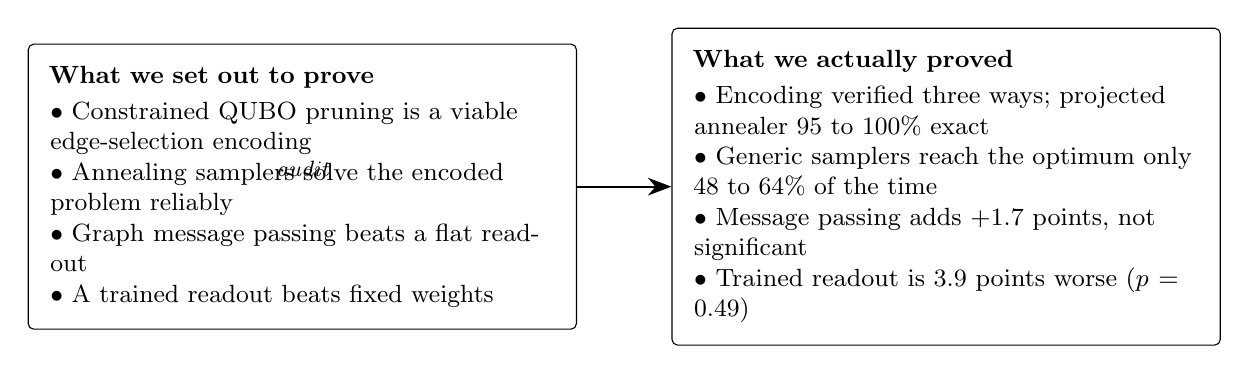
\begin{tikzpicture}[
  font=\small,
  col/.style={draw, rounded corners=2pt, inner sep=8pt, align=left,
              text width=6.4cm},
]
\node[col] (left) {%
  \textbf{What we set out to prove}\\[2pt]
  $\bullet$ Constrained QUBO pruning is a viable edge-selection encoding\\
  $\bullet$ Annealing samplers solve the encoded problem reliably\\
  $\bullet$ Graph message passing beats a flat readout\\
  $\bullet$ A trained readout beats fixed weights};
\node[col, right=1.2cm of left] (right) {%
  \textbf{What we actually proved}\\[2pt]
  $\bullet$ Encoding verified three ways; projected annealer 95 to 100\%
    exact\\
  $\bullet$ Generic samplers reach the optimum only 48 to 64\% of the time\\
  $\bullet$ Message passing adds $+1.7$ points, not significant\\
  $\bullet$ Trained readout is 3.9 points worse ($p = 0.49$)};
\draw[-{Stealth[length=3mm]}, thick] (left.east) to (right.west)
  node[midway, above, font=\footnotesize\itshape] {audit};
\end{tikzpicture}
\caption{The distance between the proposal and the audited result. Every
item on the left survived contact with measurement in a modified form; the
right column is what the evidence supports.}
\label{fig:conclusion-audit}
\end{figure}

\subsection{Lessons}

Four lessons generalise beyond this project. First, verify encodings
against independent ground truth before trusting them: our encoding survived
because it was cross-checked against re-derivation, enumeration, and an
exact solver, and that triple verification is what lets the downstream
claims stand. Second, penalty-encoded constrained QUBOs are a hard landscape
for generic samplers; the penalty barriers that enforce feasibility are
exactly what trap samplers that move in raw bit space. Third,
feasibility-aware move sets matter more than solver sophistication: the
projected annealer's advantage came from proposing only valid moves and
repairing candidates, not from a cleverer temperature schedule. Fourth,
negative results deserve the same prominence as positive ones, because the
negative results here, the MILP dominance, the threshold pruner's win, and
the readout-training null, are the findings most likely to save a future
team from repeating the same detours.

\subsection{Future work}

Several directions follow directly from what the audit exposed. The Gazebo
integration should publish velocity commands so that physics drives the
planning inputs rather than replaying scripted poses, closing the loop
between the simulator and the allocator. The browser console needs WebSocket
streaming in place of request-response stepping, plus session persistence so
long missions survive reconnects. The pruning formulation should be extended
to hierarchical or clustered variants, since connectivity is currently
enforced only up to twenty rovers due to the dense memory footprint of the
matrix. The $Q$ matrix should be run on real annealing hardware from D-Wave
to test whether the hardware changes the sampler-reliability picture that
the classical samplers painted. The readout-training null result deserves a
revisit with larger and more diverse training data, since the current
failure may be a data problem rather than a model problem. Finally, the
deterministic link-quality model should be replaced with richer radio models
that include fading and interference, which would stress the trust model in
ways the current environment cannot.

\subsection{Closing remarks}

Building this system taught the team that the distance between a plausible
pipeline and a trustworthy one is measured in verification infrastructure,
not in model complexity. The parts of the project we are most confident in
are not the cleverest components; they are the components pinned down by
independent ground truth, and the parts we trusted too early were the ones
that measurement later humbled. We set out to show that a quantum-inspired
encoding could earn its place in a rover network, and we ended up with
something more useful: a complete, audited picture of where the encoding
helps, where it does not, and exactly how much each design decision is
worth. That picture, including its negative regions, is the contribution.

\subsection{Pending items in this report}

The following placeholders remain in this report and must be completed before submission:

\begin{itemize}
  \item title page author names and date;
  \item the abstract text;
  \item Gazebo world and status-message screenshots;
  \item fleet console screenshots (orbit view, mission strip), performance capture, and demo video link;
  \item the reference list for the final section (to be supplied separately).
\end{itemize}


\section*{References}
\addcontentsline{toc}{section}{References}
\fillme{reference list for the final section; the authors will supply the
references separately. Suggested entries to confirm: Sabater and Sierra
(2005) on trust and reputation, the CBC user guide, the D-Wave sampler
documentation, the OpenJij paper, Gazebo Harmonic and ROS 2 Jazzy
documentation, and the three.js and React documentation.}

\appendix
\section{Pending Fields and Placeholders}
\label{app:pending}

This appendix collects every placeholder left in the report so that nothing
is forgotten before submission. Each entry also appears inline at the point
where the material belongs, marked as \fillme{...}.

\subsection*{Identity and front matter}
\begin{itemize}
  \item Title page: author names \fillme{author names, one per line}.
  \item Title page: submission date \fillme{submission date}.
  \item Abstract: \fillme{abstract text; 150 to 250 words}.
\end{itemize}

\subsection*{Figures and media to add}
\begin{itemize}
  \item Gazebo chapter: screenshot of the world with the four rovers.
  \item Gazebo chapter: screenshot or log excerpt of a live status message.
  \item Engine chapter: screenshot of the orbit view with link arcs visible.
  \item Engine chapter: screenshot of the mission strip during a live solver
        comparison.
  \item Engine chapter: performance capture (fps, draw calls, triangles) at
        16 rovers on the high quality tier.
  \item Engine chapter: link or QR code to a demo video.
\end{itemize}

\subsection*{Data cells to confirm}
\begin{itemize}
  \item Results chapter ablation table: confidence interval and p-value
        cells for the no-graph and random arms \fillme{CI and p for these
        two arms, if they should be printed}.
  \item Results chapter pruner table: exact success rates for the
        full-graph and top-K arms \fillme{exact rates, if they should be
        printed}.
  \item Engine chapter preset table: per-preset measured cycle times are
        currently ranges inside the measured 140 to 1420 ms span; replace
        with exact per-preset measurements if they should be printed.
\end{itemize}

\subsection*{References}
\begin{itemize}
  \item The reference list for the final section is to be supplied
        separately by the authors. See the References placeholder section.
\end{itemize}


\end{document}
